% !TEX root =main.tex
% Tipo di documento. L'uso di twoside implica che i capitoli inizino sempre con la prima pagina a sinistra, eventualmente lasciando una pagina vuota nel capitolo precedente. Se questa cosa è fastidiosa, è possibile rimuoverlo. 
\documentclass[a4paper, twoside,openright]{report}
% \documentclass[a4paper,openright]{report}

% \usepackage{fancyhdr}
% \pagestyle{fancy}
% \fancyhf{}
% \lhead{\rightmark}
% \rhead{\textbf{\thepage}}
% % \fancyfoot{}
% \setlength{\headheight}{12.5pt}
% Rimuove il numero di pagina all'inizio dei capitoli
% \fancypagestyle{plain}{
%   \fancyfoot{}
%   \fancyhead{}
%   \renewcommand{\headrulewidth}{0pt}
% }


\usepackage{graphicx} % Required for inserting images
\setkeys{Gin}{width=0.6\columnwidth}

\usepackage[utf8]{inputenc}

\usepackage{hyperref}
\usepackage{adjustbox}

\usepackage{wrapfig}

\usepackage{enumitem}
\renewcommand{\labelitemi}{$\diamond$}
\renewcommand{\labelitemiii}{$\circ$}
\setlist[enumerate,2]{label=\roman*.}
\setlist[enumerate,3]{label=(\alph*)}

\setitemize{noitemsep}
\setenumerate{noitemsep}
\setlist{noitemsep}

\usepackage{paracol}
\usepackage{multicol}
\usepackage{booktabs}


\usepackage{geometry}

\usepackage{color}

\usepackage{listings}
% \usepackage{minted}

\usepackage{amsmath}
\usepackage{amssymb}
\usepackage{amsfonts}
\usepackage{mathtools}
\usepackage{bm}
\usepackage{nicefrac, xfrac}

\usepackage{wasysym}

% Uso dei colori
\usepackage[dvipsnames,table,xcdraw]{xcolor}
\usepackage{colortbl}
\usepackage{rotating}
\usepackage{adjustbox}

\usepackage{multirow}
\usepackage{booktabs}
\usepackage{makecell}


\usepackage{tikz}
\usetikzlibrary{automata, arrows,bending}
\usetikzlibrary{positioning}
\usetikzlibrary{shapes.geometric}
\usepackage{parskip}
\usepackage{changepage}

\usepackage{soul}
\usepackage{cancel}

% This are needed because the correct double quotes would be ``'' or ``",
% but i've always written "text"
% TODO - check whether this affects listing environment
% \usepackage [english]{babel}
% \usepackage [autostyle, english = american]{csquotes}
% \MakeOuterQuote{"}

\geometry{margin=0.6in}

\setlist[description]{itemsep=0em,topsep=0.5em,parsep=0em}
\setlist[itemize]{itemsep=0em,topsep=0pt}
\setlist[enumerate]{itemsep=0em,topsep=0pt}

\hypersetup{
    colorlinks=true,
    linkcolor=black,
    filecolor=mauve,
    urlcolor=blue,
}

\definecolor{gray}{gray}{0.3}
\definecolor{verylightgray}{gray}{0.95}
\definecolor{blue}{rgb}{0,0,1}
\definecolor{mauve}{rgb}{0.58,0,0.82}
\definecolor{darkred}{rgb}{0.3,0,0}
\definecolor{darkgreen}{rgb}{0,0.3,0}
\definecolor{darkgray}{gray}{0.15}



\newenvironment{notes}{
\par
\color{gray}
\small}

\newcommand{\note}[1]{\begin{notes}{#1}\end{notes}}
\newcommand{\nl}[0]{\parskip = \baselineskip}
\newcommand{\lst}[1]{\lstinline{#1}}
\newcommand{\ra}{\xrightarrow{\hspace*{2em}}}
\newcommand{\ns}{\setlength{\parskip}{0em}}

\newlength{\currentparindent}
\newcommand{\labelitemize}[2]{
\setlength{\currentparindent}{\parindent}
\setlength{\parindent}{0pt}

\begin{minipage}{0em} % Adjust the width as needed
    \makebox[0em][c]{\rotatebox{90}{\small #1}}
\end{minipage}
\begin{minipage}{\dimexpr\columnwidth-1cm\relax}
    #2
\end{minipage}
\setlength{\parindent}{\currentparindent}
}
\newcommand{\colfill}{\vspace{\fill}}

\newcommand{\framed}[1]{
\begin{center}
\fbox{
    \begin{minipage}{0.8\columnwidth}
        #1
    \end{minipage}
}
\end{center}}

\newcommand{\framedt}[2]{
\begin{center}
\fbox{
    \begin{minipage}{0.8\columnwidth}
        \vspace*{1em}
        \begin{center}
            \textbf{\ul{#1}}
        \end{center}
        \nl
        #2
    \end{minipage}
}
\end{center}}

\newcommand{\proscons}[4]{
    \begin{paracol}{2}
        \labelitemize{\color{darkgreen}\ul{\textit{#1}}}{
           \color{darkgreen}
           #3
        }
        \switchcolumn
        \labelitemize{\color{darkred}\ul{\textit{#2}}}{
           \color{darkred}
           #4
        }
     \end{paracol}
}

\newcommand\hcancel[2][black]{\setbox0=\hbox{$#2$}%
\rlap{\raisebox{.45\ht0}{\textcolor{#1}{\rule{\wd0}{1pt}}}}#2} 


\lstset{frame=false,
 showstringspaces=false,
 breaklines=true;
 columns=flexible,
 basicstyle={\small\ttfamily},
 keywordstyle=\color{blue},
 commentstyle=\color{darkgreen},
 stringstyle=\color{mauve}
 tabsize=3
}

\newtheorem{definition}{Definition}[chapter]
\newtheorem{theorem}{Theorem}[chapter]

\usepackage{fancyhdr}
% \usepackage{nameref,autoref}

\pagestyle{fancy}
\fancyhf{}
\fancyhead[LE,RO]{\thepage} % Page number on Outer side of header on each page
\fancyhead[LO]{\leftmark} % section title on Left side of header on Odd pages
\fancyhead[RE]{\rightmark} % subection title on Right side of header on Even pages
\fancyfoot{}
\renewcommand{\headrulewidth}{0.4pt} % Width of line under the header
% \setcounter{secnumdepth}{2} % Depth of sectioning commands to include in the table of contents

% Rimuove il numero di pagina all'inizio dei capitoli
\fancypagestyle{plain}{
  \fancyfoot{}
  \fancyhead{}
  \renewcommand{\headrulewidth}{0pt}
}

\usepackage{emptypage}

% \setlength\cftsectionnumwidth{4em} % uncomment to see difference
\title{Mobile and Cyber Physical Systems - Appunti}
\author{Francesco Lorenzoni}
\date{February 2024}

% \usepackage{tocloft}
% % Adjust the spacing in the table of contents
% \cftsetpnumwidth{8em} % Width of the box containing the section numbers
% \cftsetrmarg{8em}     % Right margin

\usepackage{etoolbox}

% Add space after section number in TOC
\makeatletter
\renewcommand{\l@section}{\@dottedtocline{1}{1.5em}{2.6em}}
% \renewcommand{\l@subsection}{\@dottedtocline{2}{4em}{3.6em}}
% \renewcommand{\l@subsubsection}{\@dottedtocline{3}{7.4em}{4.5em}}
\renewcommand{\l@subsection}{\@dottedtocline{2}{2.5em}{3.6em}}
\renewcommand{\l@subsubsection}{\@dottedtocline{3}{3.5em}{4.5em}}
\makeatother

\setcounter{minitocdepth}{4}
\mtcsettitle{parttoc}{Contents of this Part} % Set the title for the part TOC

\begin{document}
% \dominitoc
\doparttoc[n]
\maketitle
\tableofcontents
% \addtocontents{toc}{\setlength{\cftsecnumwidth}{4em}}
\chapter*{Course info}
\dots
\part{Stefano Chessa}
% \minitoc
\parttoc
\chapter{Introduction}
\section*{27 - Settembre}
\section{Product based}
In \textit{Project-based SE} there is loop which nowdays cripples software since its early stages of development.
This is due to mutable nature of requirements, which often change throughout time along the features implemented by the software.
\begin{center}
\begin{tikzpicture}
    \node[draw=white,align=left] (A) at (1.5,3) {Problem};
    \node[draw=white,align=left] (B) at (0,0) {Requirements};
    \node[draw=white,align=left] (C) at (3,0) {Software};

    \path [->] (A) edge node[left] {} (B);
    \path [->] (B) edge node[left] {} (C);    
    \path [->] (C) edge node[left] {} (A);    
\end{tikzpicture}
\end{center}

\textit{Product-based SE} is opposed to \textit{Project-based SE} and the above pictures changes as follows.

\begin{center}
\begin{tikzpicture}
    \node[draw=white,align=left] (A) at (1.5,3) {Opportunity};
    \node[draw=white,align=left] (B) at (0,0) {Features};
    \node[draw=white,align=left] (C) at (3,0) {Software};

    \path [->] (A) edge node[left] {} (B);
    \path [->] (B) edge node[left] {} (C);    
    \path [->] (C) edge node[left] {} (A);    
\end{tikzpicture}
\end{center}

\section{Agile}
Agile is a collection of principles and methods applied in the software development field.
\nl

Opposed to project-based SE, in Agile the client is requested to express the requirements not in technical terms but in features.

Agile suggests an incremental development model

\subsection*{Principles}
\begin{enumerate}
    \label{subsec:agile_principles}
    \item Satisfy customer through early and continuous delivery of valuable software
    \item Welcome changing requirement, even late in development.
    Agile processes harness change for the customer's comptetitive advantage
    \item Deliver working software frequently, from a couple of weeks to a couple of months, with a preference to the shorter timescale
    \item Business people and devs must work together daily throughout the prokect
    \item Build porjects around motivated individuals and give them the environment and support they need
    \item The most efficient and effective method of conveying information to and within a dev team is face-to-face conversation
    \item Working software is the primary measure of progress
    \item Agile processes promote sustainable dev 
    \item Continuous attention to technical excellence and good design enhances agility
    \item Simplicity i.e. art of maximizing the amount of work not done is essential
    \item The best architectures, requirements, and designs emerge from self-organizing teams.
\end{enumerate}

Extreme Programming was proposed as part of the agile methodology

\section{Scrum}
Since requirements changes are rather frequent, long-term plans are unreliable,
hence SE aims to formulate short-term plans.

Scrum is found on \textbf{empiricism} and \textbf{lean thinking}; it asserts that knowledge comes from experience, and that decisions should be made on observations.

Other key terms are code \textbf{Transparency} among the team and with the customer, \textbf{Inspection} of produced code and software (artifacts), \textbf{Adaptation} to changes in features and requirements.

The \textbf{Scrum Team} is composed by:
\begin{enumerate}
    \item \textbf{Product Owner}: must ensure that the dev team is always focused on the goal
    \item \textbf{Scrum Master}: Scrum expert which drives the team to apply properly the Scrum framework.
    \item \textbf{Developers}: actual monkeys people which write code
\end{enumerate}

In scrum SW is developed in \textbf{sprints}, i.e. fixed-length periods with a specific goal to be achieved.

\begin{itemize}
    \item Product backlog: to-do list of items to be implemented
    \item Timeboxed sprints
    \item Self-organizing teams
\end{itemize}

...
\textbf{Prod Backlog Revised}\\
\textbf{PBI Estimation Metrics}

\subsection{Timeboxed Sprints}
Even if at the end of a srpint the goal hasn't been reached, "no worries", the work stops anyway;
there will be a new sprint which will include the work which has not been implemented in the previous one.

\subsection{Scrum Meetings}

\subsection{Agile activities}
Test automation
Continuous integration

\subsection{Sprint reviews}
At the end of each sprint there is a review meeting which involves the \textit{whole} team.
The \textit{product owner} has the ultimate authority to decide wether the sprint goal has been reached or not.
The sprint review should include a process review, in which the whole team shares ideas on how to improve their way of working.

\textbf{Team size}\nl

\section{5 - Ottobre}



\chapter{IEEE 802.11}

\begin{figure}[htbp]
   \centering
   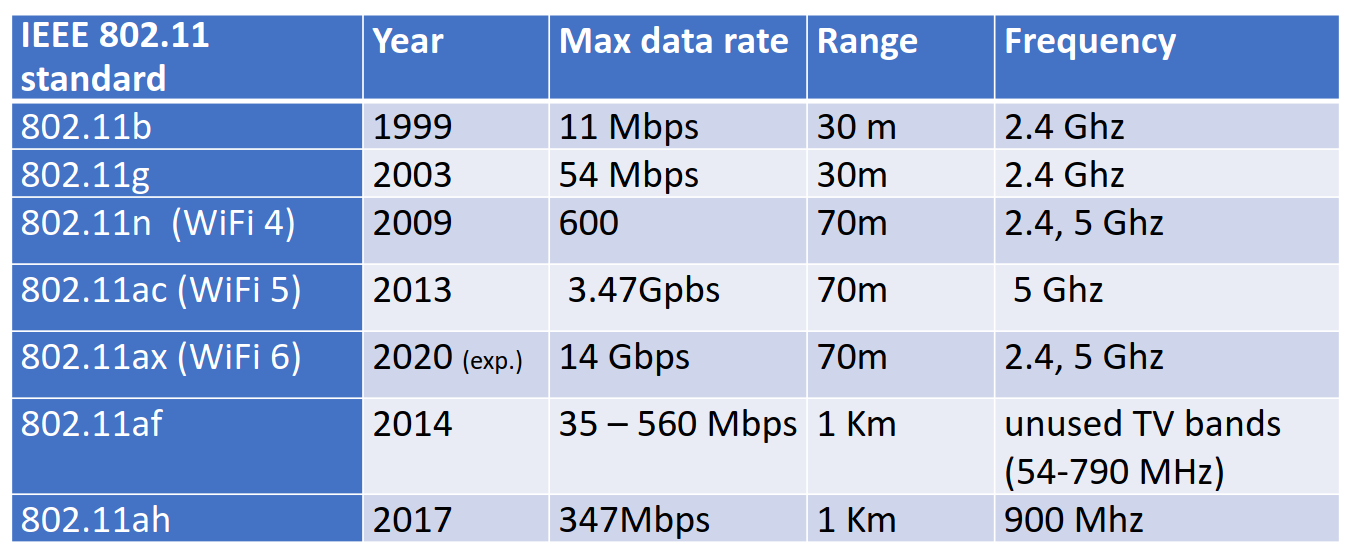
\includegraphics{images/ieee_bgn.png}
   \caption{IEEE 802.11 standards}
   \label{fig:ieee_bgn}
   All these standards \texttt{use \texttt{CSMA/CA} for multiple access}, and have base-station and ad-hoc network versions
\end{figure}

IEEE 802.11 standards refer to the \textit{Physical} Layer.
In case of an AP (Access Point), every station must channel its communication through the AP to talk to any other. Otherwise, in an \textit{Ad-Hoc} network, stations can communicate directly with each other.

TODO

\note{TODO non ci sono domande su questa cose nel pdf}
\chapter{Fabric}
``Fabric'' is the term used to refer to the \textit{interconnection} between nodes of a datacenter.\\
\ul{Cabling is of paramount importance.}
\note{Prof. Cisternino learnt it ``the hard way'' when he performed the cabling of the first UniPi datacenter by himself}
\begin{enumerate}
   \item Maintenance
   \item Cooling
   \begin{enumerate}
      \item Cables may heat up
      \item Cables may obstruct air flow
   \end{enumerate}
   \item Determines which machines interact with each other (\textit{fabric})
   \item Bandwidth
   \item Not neglectable cost
\end{enumerate}

We refer to North-South traffic indicating the traffic outgoing and incoming to the datacenter (internet), while we refer to East-West as the internal traffic between servers.
Most of the network (or fabric) traffic is processed horizontally (North-South traffic)\footnote{Seems odd that ``horizontal'' refers to North-South traffic, but that's how it is.}.


\section{Bandwidth and Storage implications}
\label{sec:bandwidth_storage}
A standard datacenter has servers connected with 25Gbit links in both directions, summing up to 50Gbit total bandwidth.
Current SSDs using NVMe provide much more, about $3.5 GB/s$, making \ul{4 drives are enough to saturate a 100Gbit/s link.}\\
We moved from a situation where the \textbf{bottleneck} were slow Hard Drives, to the current one where the bottleneck is the ---network--- \textbf{bandwidth}.\\
Recently the PCI 3.0, which lasted very long ---providing roughly$\sim\texttt{120Gbit/s}$ using 16 pin---, suddenly become unsufficient to handle the needed traffic.

Considering this, \ul{datacenters must be designed to allow \textit{Terabytes} of data to be moved in east-west traffic.}

\begin{center}
   \ul{\textit{The \textbf{fabric} is the glue that makes the datacenter possible.}}
\end{center}

Besides, a single server is \textit{unable} to handle 10TBs of data and handling requests from 3000 users simultaneously. It is necessary to \textbf{distribute} the requests.

HDDs are still currently used for \textbf{cold storage};
CPUs will access data exclusively from SSDs, and sometimes the server is shipped with on board \textbf{full-flash storage}.\\
The difference in price between SSDs and HDDs becomes negligible since you pay for top CPU, top GPU, top RAM;
furthermore, you can't waste ---the high amount of--- energy ---consumed by such components--- by waiting for a slow drive.

SSDs have a known write limit, but today, the usually last enough time: if you write the whole disk every day it will last for 5 years. Most-likely after five years you'd have to renew some components anyway, besides the failure is a predictable event.

\section{Cables and standards}
\subsection{Optical}
Electric current propagates at a speed $s = {\sim}0.6c$.
Hence \textbf{optical fiber} is ---at least in theory?--- faster.

\textbf{Lasers} are a coherent beam of equal fotons. It is possible to transfer energy through such fotons. Something resembling a laser is used for optical fibers.

Blu-Ray came out when scientists managed to create light using frequencies in the Blu area, which are the higher ones.
Currently, the best and most expensive optical fibers exploit blu-lasers as source of light.

Note that with optical you always need 2 fibers, one sending and the other receiving. The two possible connectors are \texttt{SC} and \texttt{LC}.
Sometimes the two ends of the cable are detachable so that the cables may be switched; this is useful because sometimes you may want to attach the TX cable on the RX plug and viceversa. 

\begin{figure}[htbp]
   \centering
   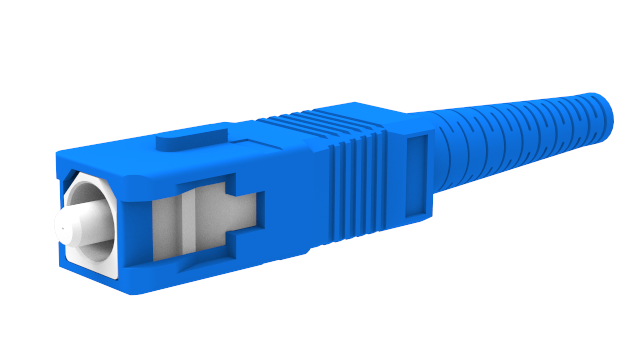
\includegraphics[width=0.25\columnwidth]{images/SC.png}
   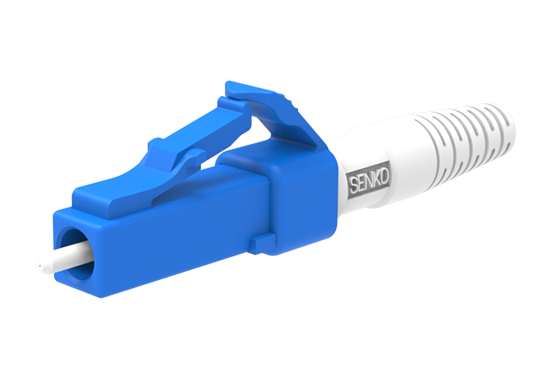
\includegraphics[width=0.25\columnwidth]{images/LC.png}
   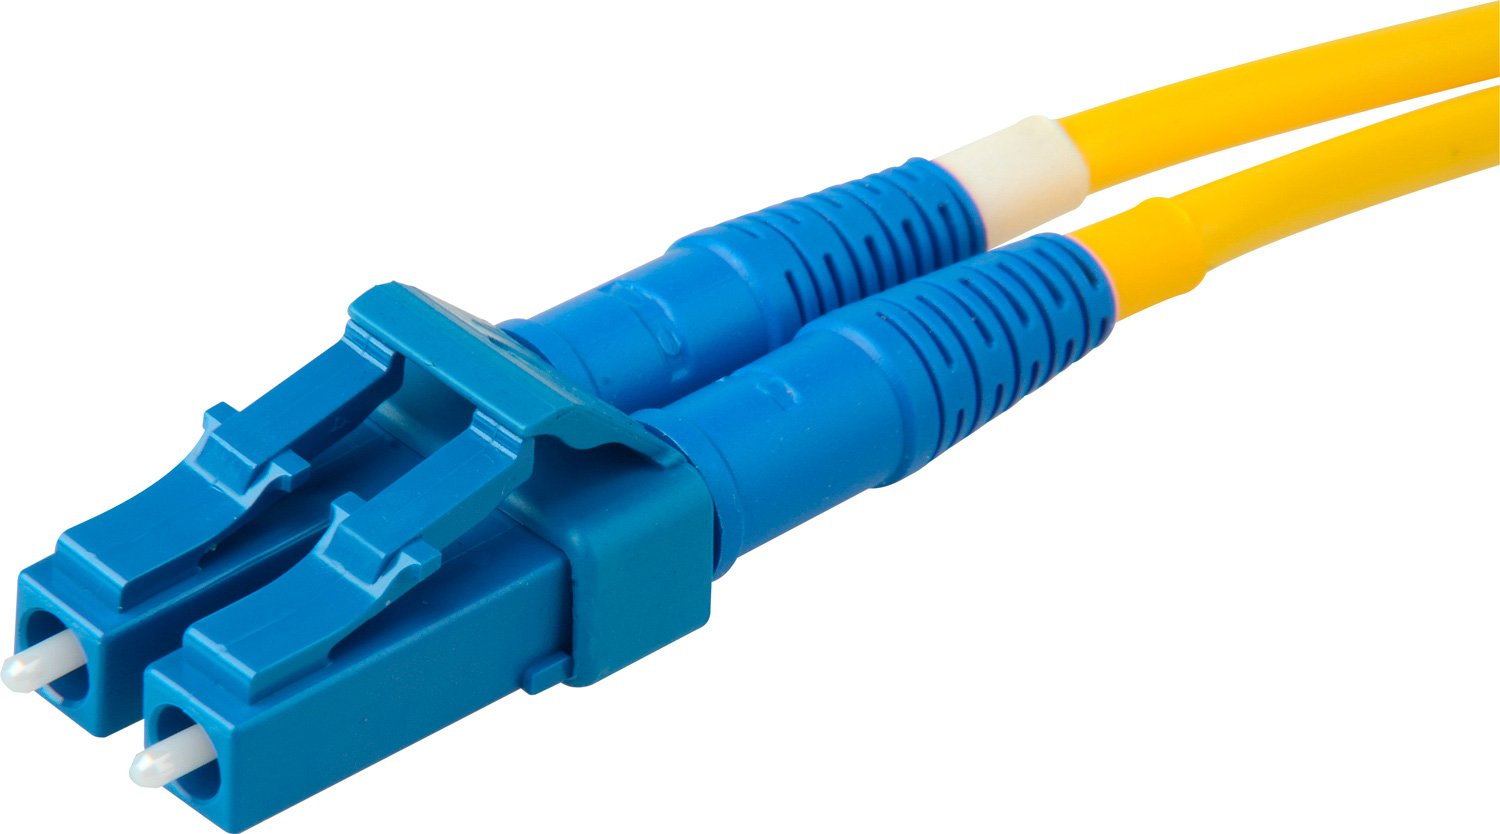
\includegraphics[width=0.25\columnwidth]{images/LC_coupled.JPG}
   \caption{\texttt{SC} and \texttt{LC} connectors}
   \label{fig:sc_lc_connectors}
\end{figure}

\subsection{Copper wires}
In case of electricity there are many aspects to be considered. Interferences, cable diameter/size, length, and also the fact that if a \texttt{1} has been transmitted for some time, it takes longer to transmit a \texttt{0}, due to the \textit{commutation} that must happen.
\nl

\begin{paracol}{2}
   \colfill
   \textbf{RJ45} is a standard physical interfaced for copper wires, which allows up to 1Gbit regularly.
   The \texttt{Cat 7} cables still use the RJ45 as connector and provide instead 10Gbit/s, but are very uncomfortable, they are so thick that they are difficult to bend.
   
   It is estimated that there have been installed $70 \times 10^9m$ of Ethernet cables, making them the most used.
   \colfill
   \switchcolumn

   \begin{figure}[htbp]
      \centering
      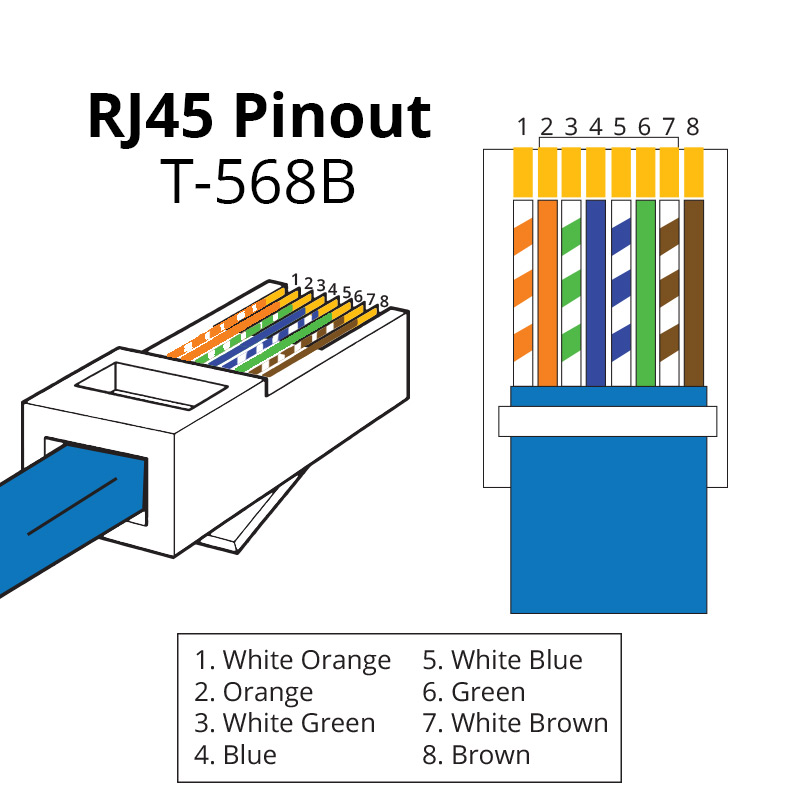
\includegraphics{images/RJ45_T568B.jpg}
      \caption{RJ45 - T568B}
      \label{fig:RJ45_T568B}
   \end{figure}
\end{paracol}

\subsection{SFP - Small Form-factor Pluggable}
There can be a cable with a LC in one side and a SC on the other side.
Instead of making switches with the optical plugs, switches were created with electrical plugs that would be able to host a \textbf{standard transceiver}.
The latter is a pluggable module that will receive current power and electrical signals for the transmission, which is responsible for transitioning between electrical signals and Optical signal (and viceversa).

\begin{paracol}{2}
   
   The aim of SFP is to decouple the optical transceivers from the server modules.
   \note{Is this correct?}
   They allow to go \textit{optic-copper}, \textit{copper-optic}, \textit{optic-optic} and \textit{copper-copper}.\\
   SFP and GBIC (oldest one, now dead) pluggable modules acting as active transceivers for optical wiring using RJ45 connector.\\
   \ul{A single cable having SFP ends costs about 100€}.
   The cost ain't neglectable \smiley.
   \note{\begin{itemize}
      \item[\texttt{SFP}] $\longrightarrow 1Gbit $
      \item[\texttt{SFP+}] $\longrightarrow 10Gbit $
      \item[\texttt{SFP28}] $\longrightarrow 25Gbit$
      \note{This is the current standard}
      \item[\texttt{QSFP28}] $\longrightarrow 4\times25Gbit$
   \end{itemize}}


   \switchcolumn

   \begin{figure}[htbp]
      \centering
      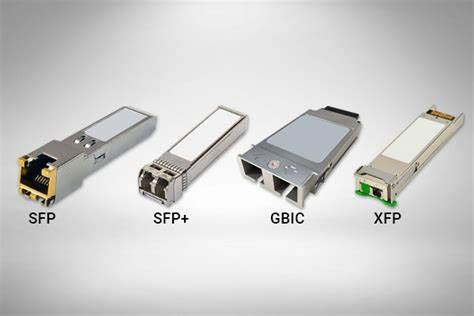
\includegraphics{images/sfp.jpeg}
      \caption{SFP transceivers form factors}
      \label{fig:sfp}
   \end{figure}
\end{paracol}

\note{Fun fact: ci sono 9 cavi USB-C e solo due portano informazioni video.}

\subsubsection{Issues about cabling and fabric}
The key point is that it would be desirable for cabling to be reconfigurable, that's why transceivers are so important.

\note{There are things called \textit{``Muffole''}, which are used for joining optical fiber cables, allowing for longer distances to be covered.
They are designed to be underground.}

Data traffic is always at least SFP+.
Current standard is SFP28. Various SFP are typically compatible, the shape of the plug should stay the same.
On switches there also some ports which are \texttt{QSFP+} or \texttt{QSFP28}, which allow up to \texttt{40} and \texttt{100Gbit/s} respecitively, and are used for north-south traffic.
\note{The \texttt{Q} letter stands for \textit{Quality}}

Switches for datacenters should be \textbf{non-blocking}, meaning that no port has to wait for other ones ---or any other thing--- before transmitting, they can also transmit simultaneously.


\ul{In every datacenter it is \textit{MANDATORY} to document the cabling.}

\subsection{InfiniBand}
Even though Ethernet is famous, it is not the only standard. InfiniBand is another one, which is used in supercomputers and known for its very high throughput and very low latency ($\sim 2\mu s$).
It may send messages up to 2GB each, with 16 priority levels.
It is a \textit{lossless protocol}, meaning that if a packet is received, its integrity is guaranteed.

\textit{IB} avoids TCP/IP stack, which is very heavy, and instead uses MPI (\textit{Message Passing Interface}), which is a way to distributed parallel programs, also exploited by OmniPath.

InfiniBand cables and connectors look similar to Ethernet ones, but they are not compatible.

Aside from HPC environments, it is uncommon to build an entire network with InfiniBand, typically there is an IB switch to whom the servers equipped with IB NICs are connected, which intereacts with the rest of the network with Ethernet, because ``it's cheaper and it works''.
\note{Today, we are about 400 Gbit/s on both IB and Ethernet.}

\subsection{RDMA - Remote Direct Memory Access}

RDMA is a technology API based (not a protocol!) that allows to access memory of a remote machine without involving the CPU or the OS of the remote machine.

RDMA supports zero-copy networking by enabling the network adapter to transfer data directly to or from application memory, eliminating the need to copy data between application memory and the data buffers in the operating system.\\
The main use case is distributed storage.

RoCE (\textit{RDMA over Converged Ethernet}) is a network protocol that allows remote direct memory access (RDMA) over an Ethernet network.

\subsection{Omni-Path}
Omni-Path is a high-performance computing network architecture, developed by Intel. It is a successor to Intel's InfiniBand, and competes with InfiniBand's EDR and HDR technologies.

Intel plans to develop technology that will serve as the on-ramp to \textit{exascale computing}\footnote{A computing system capable of the least one exaFLOPS}, which is the next frontier in high-performance computing.


\chapter{BitTorrent}

The goal of \textit{Content Distribution Networks} is to distribute web contents to hundreds of thousands or millions
of simultaneous users, \ul{exploiting data and/or service \textbf{replication} on different \textbf{mirror servers}}.

In \textbf{P2P CDN} the initial file request are served by a centralized server, and further requests served by peers which have already received and replicated the files (\textbf{\textit{seeders}}), without involving the initial server.

\begin{center}
\fbox{
   \begin{minipage}{0.8\columnwidth}
      \nl
      \begin{center}
         \ul{\textbf{BitTorrent} in a nutshell}
      \end{center}
      \nl

      \begin{itemize}
         \item Basically a \textit{Content Distribution Network} (\texttt{CDN})
         \item A distributed set of hosts cooperating to distribute large data set to end users.
         \item Efficient content distribution systems using \textit{file swarming}
         \item Does \textit{not} perform all the functions of a typical P2P system, like searching
         \item Rather than providing a search protocol itself, was designed to integrate seamlessly with the Web and made file descriptors available via Web, which could be searched with standard Web search
         \item \textit{File swarming}: a peer makes whatever portion of the file that is downloaded immediately available for sharing
      \end{itemize}
   \end{minipage}  
   }
\end{center}

\section{Deeper into BitTorrent}
\begin{figure}[htbp]
   \centering
   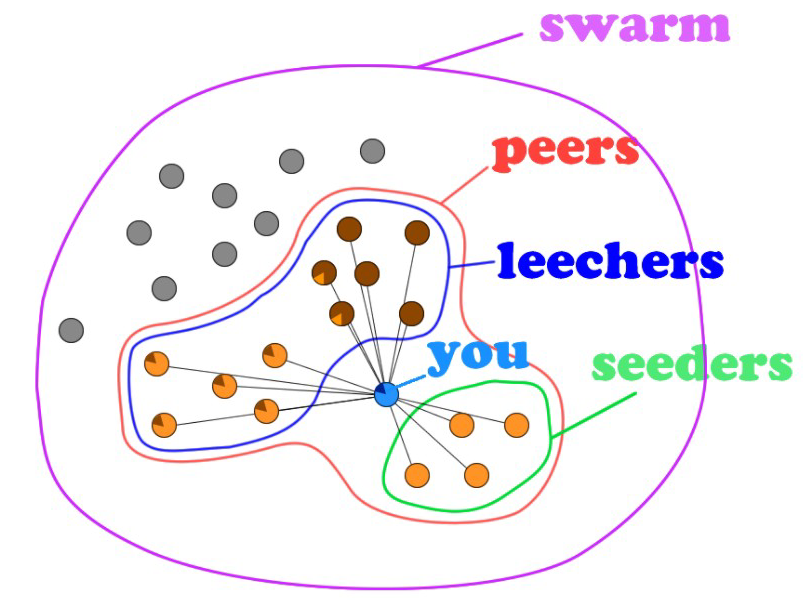
\includegraphics{images/bit_swarmschema.png}
   \caption{Swarm schema}
   \label{fig:bit_swarmschema}
\end{figure}
\subsection{Glossary}
\begin{itemize}
   \item \textbf{tracker}: active entity which coordinates
   the peers sharing the file, taking trace of who is currently providing the content
   \note{\begin{itemize}
      \item Joe connects to the tracker announcing the content
      \item the tracker now knows Joe is providing the file
   \end{itemize}}
   \item \texttt{.torrent} a descriptor of the file to be published on a server, which includes a reference to a tracker
   \item \textbf{swarm} set of peers collaborating to the distribution of the same file coordinated by the same tracker
   \item \textbf{seeder} peer which owns all the parts of the file
   \item \textbf{leecher} peer which has some part or no part of the file and downloads the file from the seeders and/or from other lechers.
\end{itemize}

\subsection{Protocol Overview}
\begin{figure}[htbp]
   \centering
   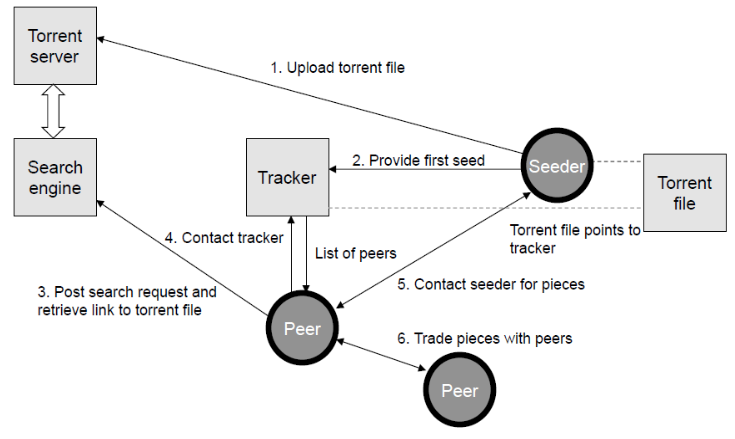
\includegraphics{images/bit_overview.png}
   \caption{BitTorrent protocol overview}
   \label{fig:bit_overview}
   BitTorrent protocol is built on top of HTTP
\end{figure}
\labelitemize{\textit{Seeder}}{
   \begin{enumerate}
      \item Upload the .torrent on a Torrent Server
      \item Opens a connection to the Tracker and informs it of its own existence: for the moment, it is the only peer which owns the file
   \end{enumerate}
}
\labelitemize{\textit{Peers}}{
   \begin{enumerate}
      \setcounter{enumi}{2}
      \item Retrieves the file descriptor (.torrent) and opens it through the BitTorrent
      client
      \item Opens a connection to the tracker and informs it of its own existence and
      receives from the tracker a list of peers of the swarm
      \item Opens a set of connections with other peers of the swarm.
   \end{enumerate}
}

Objects are serialized in \textbf{Bencode}, which is ---not popular as \texttt{JSON}--- used only in torrent; provides 4 data types: String, Integer, Lists and Dictionaries.\\
Content is split into chunks called pieces (256KB - 2MB):
when a peer receives a piece, it becomes the seeder of that piece.
\note{
   \ns
      There is a SHA-1 hash per piece stored in the .torrent file, used to check the piece once it is fully downloaded, 
      allowing to require retransmission in case the check fails.\\
      Pieces size got adapted to have a reasonably small .torrent file
}
Pieces are then split in \textbf{subpieces} (\textit{\textbf{blocks}}) of 16KB, with each one downloadable from a different peer, optimizing the bandwith and allowing \textit{pipelining}, decreasing the overall download time.

Trackers keep a database of swarms identified by torrent hash, and knows also the state of each peer in each swarm.
In the last versions, \textbf{trackerless} BitTorrent uses \textit{Kademlia DHT} to avoid the centralization point of the tracker.

\section{Pieces selection}
The order in which pieces are selected by different peers is critical for good performance, to avoid making peers end up stuck with the same pieces.
\labelitemize{\textit{Policies}}{
   \begin{itemize}
      \item \textbf{Strict Priority}\\
      Complete the ``assembling'' of a piece before asking for another piece
      \item \textbf{Rarest First}\\
      Download the rarest pieces first
      \item \textbf{Random First Piece}\\
      Choose a random piece ---only--- in the bootstrap phase
      \item \textbf{Endgame}\\
      When the file download is almost terminated, the remaining pieces are required in \textit{parallel} to all peers who own them.
      This policy is executed for a small period of time
   \end{itemize}
}

\subsection{Free Riders}
Free riders in BitTorrent are peers that do not put their bandwidth at disposal of the community.\\
Several non official BitTorrent clients enable the user to limit the upload bandwidth as they like.

However, an approach to solve this problem is based on \textbf{reciprocity}, allowing a client to obtain a good service if and only if it gives a good service to the community, by exploiting a dynamic strategy based on connection monitoring called ``Tit for Tat'', implemented using \textbf{choking}:\\
choking means \textit{temporarily} refusing to upload to another peer, but still downloading from them;  
the principle is to upload to peers who have uploaded to us.

\labelitemize{\textit{Choking}}{
\begin{center}
   \textit{The local peer can receive data from a remote peer if}
   \begin{itemize}
      \item The local peer is \textit{interested} in the remote peer
      \item The remote peer \textit{unchoked} the local peer
   \end{itemize}
\end{center}
   }

Choking only peers that upload the most to the local peers would lead to ignoring peers that recently join the network
and to the lack of discovery of connections actually better than the used ones.\\
To avoid this, BitTorrent uses \textbf{optimistic unchoking}, i.e. \ul{one random peer is being unchoked}.\\
Then, every 30s an interested and choked peer is selected at random \textbf{planned optimistic unchoke} (\texttt{POU}), and if this new connection turns out to be better than one of the existing
unchoked connections, it will replace it.

In case a peer is chocked by everyone, it follows an \textbf{anti-snubbing} policy, by increasing the number of simultaneous optimistic
unchocke to more than one.

For \textit{seeders} this schema does clearly not apply, since they do not have to download anything; hence they use a different choking algorithm:
\ul{unchoke peers with the highest upload rate}, ensuring that pieces get uploaded and replicated faster.

\section{DHT and BitTorrent}
Kademlia is the protocol used by the largest public DHTs.
Bittorrent Inc. introduces its own DHT, called \textit{Mainline DHT}.
With respect to Kademlia there are some improvements concerning 
\begin{itemize}
   \item Routing table management
   \item Look-up
\end{itemize}

The main purpose of Mainline DHT is to provide a “trackerless” peer discovery mechanism to locate peers belonging to a swarm.
\chapter{Storage}

\framedt{Data Loss}{
   \textit{``Storage is crucial because, if a switch fails, or a server fails, the service will be interrupted, but the data will still be there. \ul{If the storage fails, the \textbf{data will be lost}}.''}
   -Prof. Cisternino\\

   \textbf{Data} is the most important of a system. Since data loss is \textbf{permanent}, the storage is completely different from computing or networking.
}

\begin{paracol}{2}
   \colfill
   Historically the storage was the slowest part of the system, \textit{ms} against \textit{ns} of the CPU.
   Today, with SSDs, the gap is considerably reduced to \textit{$\mu s$}, they are $\sim 100x$ times faster.
   
   \ul{NVMe stands for \textit{Non-Volatile Memory Express}, and is a protocol (\textit{not a HW component!})} that allows to access the storage directly from the PCIe bus, without having to go through the SATA controller. This allows to have a much higher throughput, and a much lower latency.

   \note{Optane was a technology developed by intel which is now end of life}

   \colfill
   \switchcolumn

   \begin{figure}[htbp]
      \centering
      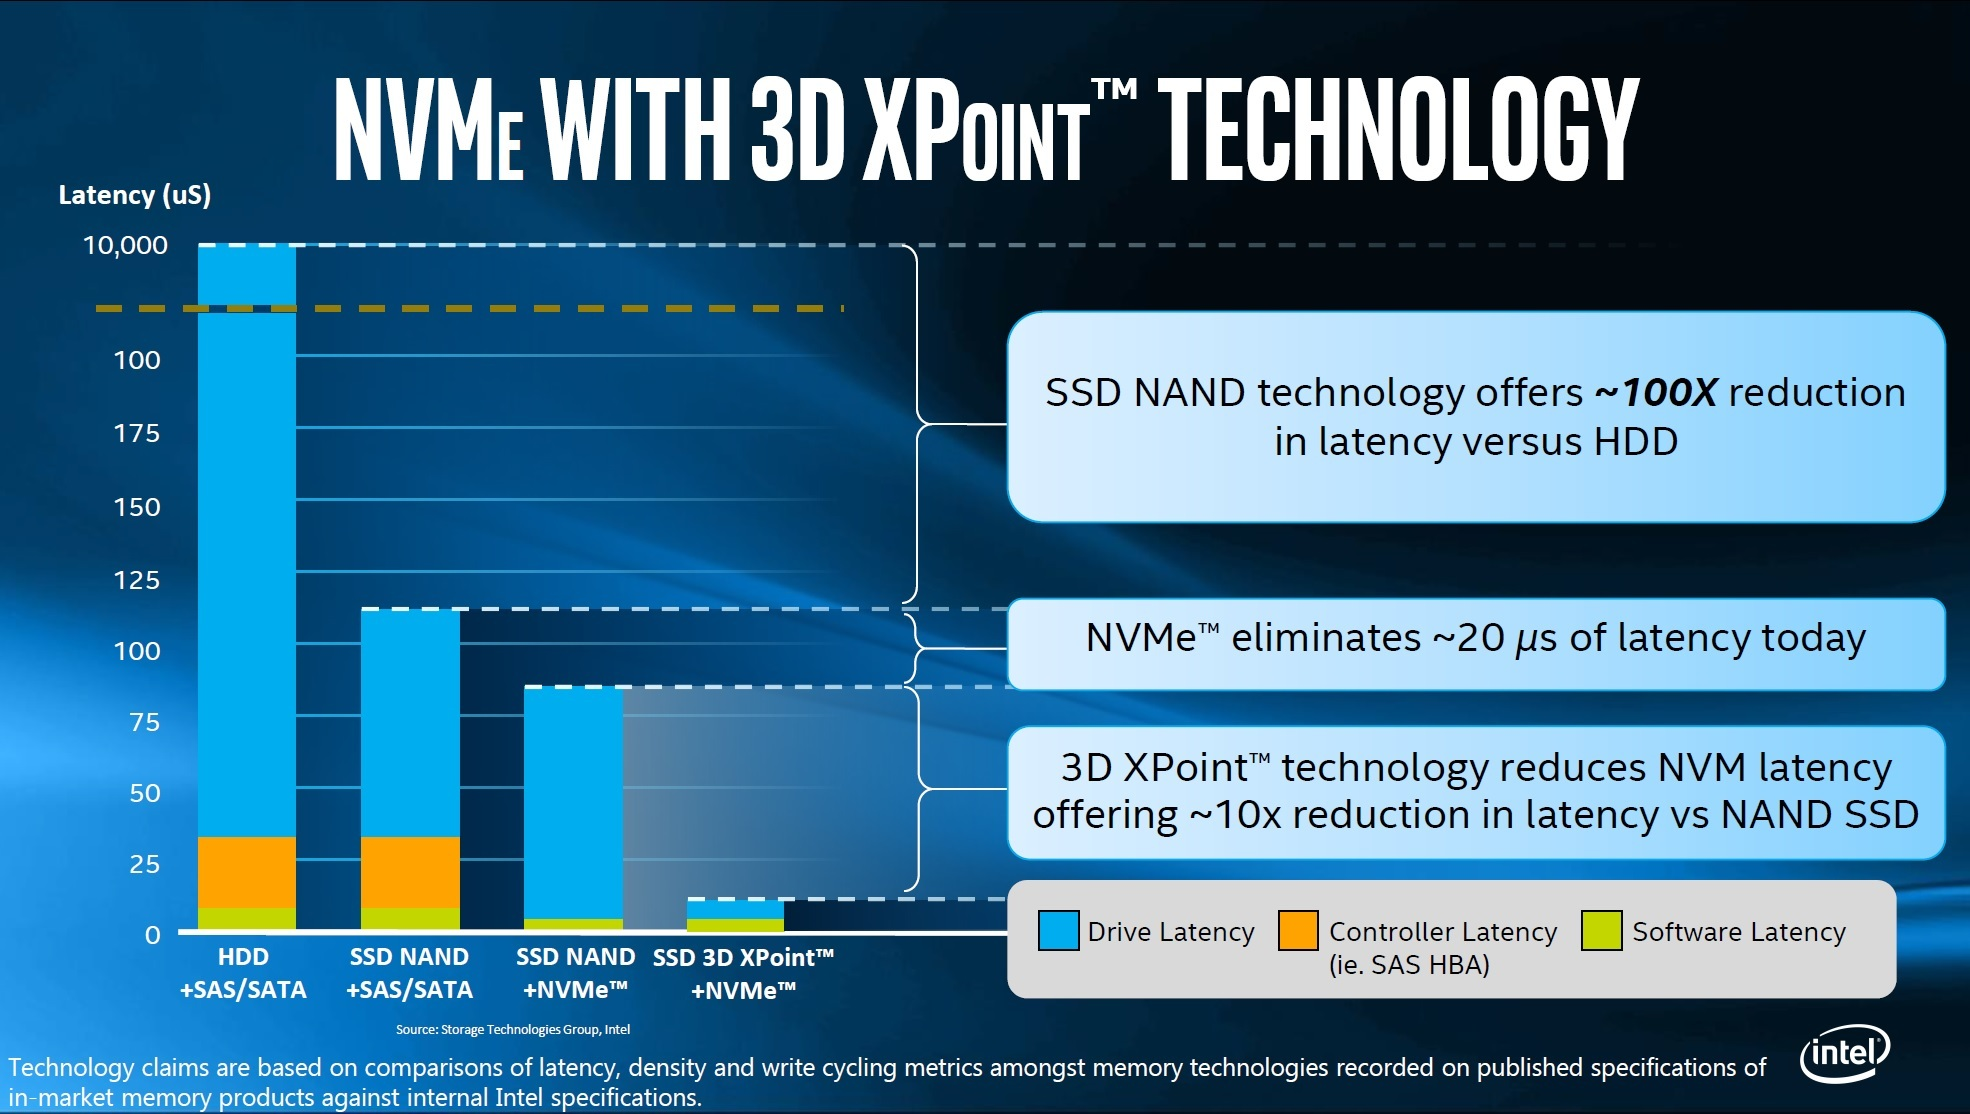
\includegraphics{images/storage_intel.jpg}
      \caption{Storage types comparison}
      \label{fig:storage_intel}
      NVMe basically removes the orange part of the figure, which is the latency introduced by the controller, since it is a \textit{controller-less protocol} and allows to access the storage directly from the PCIe bus.
   \end{figure}
\end{paracol}


\framedt{
   \textit{Why would a 15TB disk be better than a 27TB disk?}\\
   }{
      \note{Assume the same performance, and the same price.}
      It would be preferrable because \ul{it would take less time to extract all the data from the disk}\footnotemark[1], since it is smaller.
      
      However, large capacity drives are used for \textit{cold storage}, where the data is not accessed frequently, speed is not a priority, and even if the data is accessed, only a portion of the disk is needed at a time; in case of failure and thus needing to retrieve an entire backup, the time taken to retrieve the data is not a priority, since this ---hopefully--- happens only ``once''.
      }
      
\footnotetext[1]{i.e. taking advantage of the space provided}
\section{SSDs - QLC and TLC}
SSDs were invented by Toshiba back in 1980, but they were not popular for almost 30 years, until they eventually became cost-effective. Sometimes extra size in SSDs is used for redundancy, to increase the lifespan of the disk e.g. on a 30TB disk, only 10TB are used, the rest is used for redundancy, extending x3 the lifespan of the disk.

\note{DWPD stands for \textit{Drive Writes Per Day}, and is a measure of how many times the disk can be written to in a day. It can be calculated as $\frac{TBW}{365\times\textit{Years of Warranty}\times\textit{capacity}}$}.

TLC stands for \textit{Triple Level Cell}, and QLC stands for \textit{Quad Level Cell}. The difference between the two is the number of bits stored in each cell. The more bits stored in each cell, the cheaper the disk is, but the slower it is. The more bits stored in each cell, the more difficult it is to read and write the data, and the more difficult it is to keep the data stored in the cell.

Generally QLC disks are used for cold storage, while TLC disks are used for hot storage.
TLC in general is more reliable than QLC, has a longer lifespan and better performance, however they cost more.

\section{Storage Concepts}
\subsection{Tiering - Memory Hierarchy}

\begin{figure}[htbp]
   \centering
   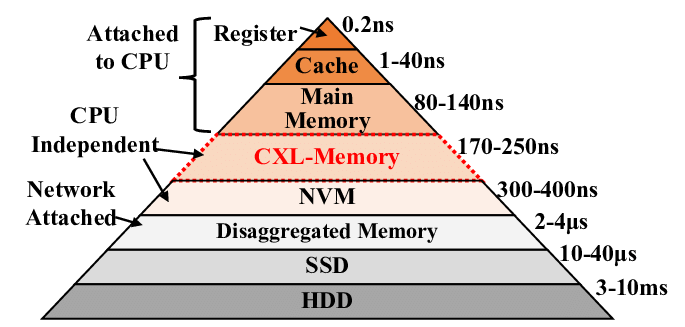
\includegraphics{images/tiering_memory.png}
   \caption{Memory tiering hierarchy}
   Ram could actually be split in \texttt{RAM} and \texttt{nvRAM} (Non-volatile \texttt{RAM}, uses \texttt{nvDIMM}), which is used to store the data in case of a power failure.
   Sometimes, \textit{tape} is included in the hierarchy, because it is used for long-term storage, and it is very cheap.
   \label{fig:tiering_memory}
\end{figure}

Tiering consists in categorizing the data in different categories, and storing the data in different types of storage, depending on the category. The data that is accessed more frequently is stored in the fastest storage, while the data that is accessed less frequently is stored in the slowest storage. This allows to increase the performance, and to reduce the cost. 

\subsection{IO operations, are they all the same?}
\textbf{IOPS} (Input/output operations per second) is an input/output
performance metric used to characterize computer storage devices; it is associated with an access pattern: \textit{random} or \textit{sequential}.

\subsubsection{Random vs Sequential access}

Before explaining the distinction, is important to remember the concept of \textit{queues}: for each thread, the OS can implement a series of queues to solve asynchronously the I/O requests. Using multiple queue can make performances better, since having
the OS to manage parallel requests will increase throughput.
If the queries are latency sensible, not using a queue is better, since
it allows a single query to have ``max'' priority.

\textit{Random access files} are advantageous in scenarios where frequent direct access or modification of specific records is required, while \textit{sequential access files} are advantageous in scenarios where frequent reads of the full files are required. The disk behaves differntly in case of access of those files.

To have a full picture of random vs sequential access, check this site: \url{https://www.prepbytes.com/blog/general/difference-between-sequential-and-random-access-file/} 

\newpage
\subsubsection{Cisternino's demo}
Prof. Cisternino showed a demo in class, where he used a tool to measure the IOPS of a disk.
\begin{figure}[htbp]
   \centering
   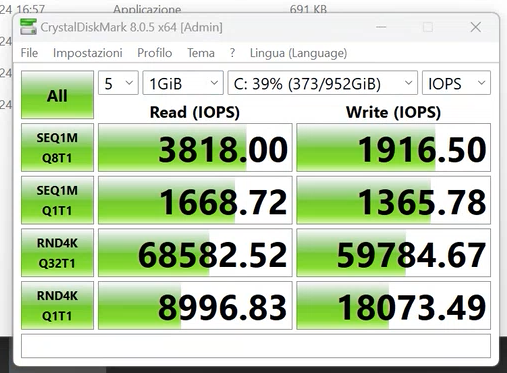
\includegraphics{images/iops.png}
   \caption{IOPS demo; respetively}
   \label{fig:iops}
\end{figure}

\ul{Recall that IOPS by itself is meaningless!} It is a number that must qualified and put in relationship with something else.

\subsection{Latency and Storage Aggregation}
A mechanical hard drive introduces 2.71\% of latency when reading, for instance, 40MB of data.  Optane can perform 416 accesses in the same time needed by a mechanical hard drive to perform 1 access. It looks like the latency in this latter case is neglegtible. Someone may be tempted to reduce the size of read/write operations and perform multiple smaller ones, since ``it's free''. 

Latency in general is due to:
\begin{itemize}
   \item \textbf{Software}\\
   $\mu s$ order which cannot be removed
   \item \textbf{Controller}\\
   Taken down to $20\mu s$ with NVMe (even $2.8\mu s$ according to Copilot)
   \item \textbf{HDD latency}\\
   This was drastically reduced with SSDs and got even less with 3D NAND.
\end{itemize}
Latency may be solved by \textbf{storage aggregation}, which consists in aggregating multiple storage devices into a single logical unit, in order to increase the performance and reliability.
Even if the data is split in multiple disks, the whole system is ``pictured'' as a single huge drive\footnote{\textit{``Cloud resource pooling''} rings a bell?}, making a huge difference in terms of latency, since multiple \texttt{read/write} requests may be sent in parallel to multiple disks.

\newpage
\subsection{Storage Fabric - Fibre Channel}
\textbf{Fibre Channel} is the fabric dedicated to storage; the link coming from the storage ends up in the \textit{HBA} (Host Bus Adapter) in the server.
\begin{paracol}{2}

   \colfill
   The idea is to have an interface which announces itself as drive and that manages the remote storage through Fibre Channel.
   Fibre Channel typically runs on optical fiber cables, but may also run on Ethernet cables (FCoE).

   In Fig. \ref{fig:fibrechannel} is depicted the ideal architecture for Fibre Channel, where the storage is connected to the network through a switch, and the servers have a dedicated HBA to connect to the storage.
   \colfill
   
   \switchcolumn
   \begin{figure}[htbp]
      \centering
      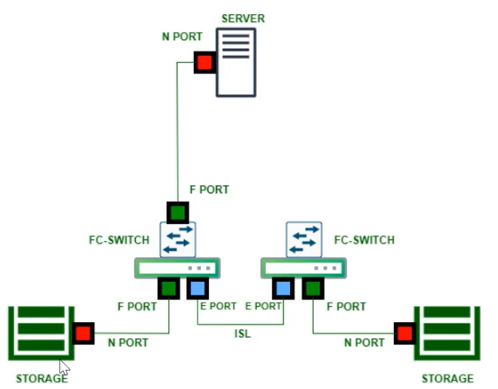
\includegraphics{images/fibrechannel.png}
      \caption{Fibre Channel desired architecture}
      \label{fig:fibrechannel}
   \end{figure}
   
\end{paracol}

\begin{figure}[htbp]
   \centering
   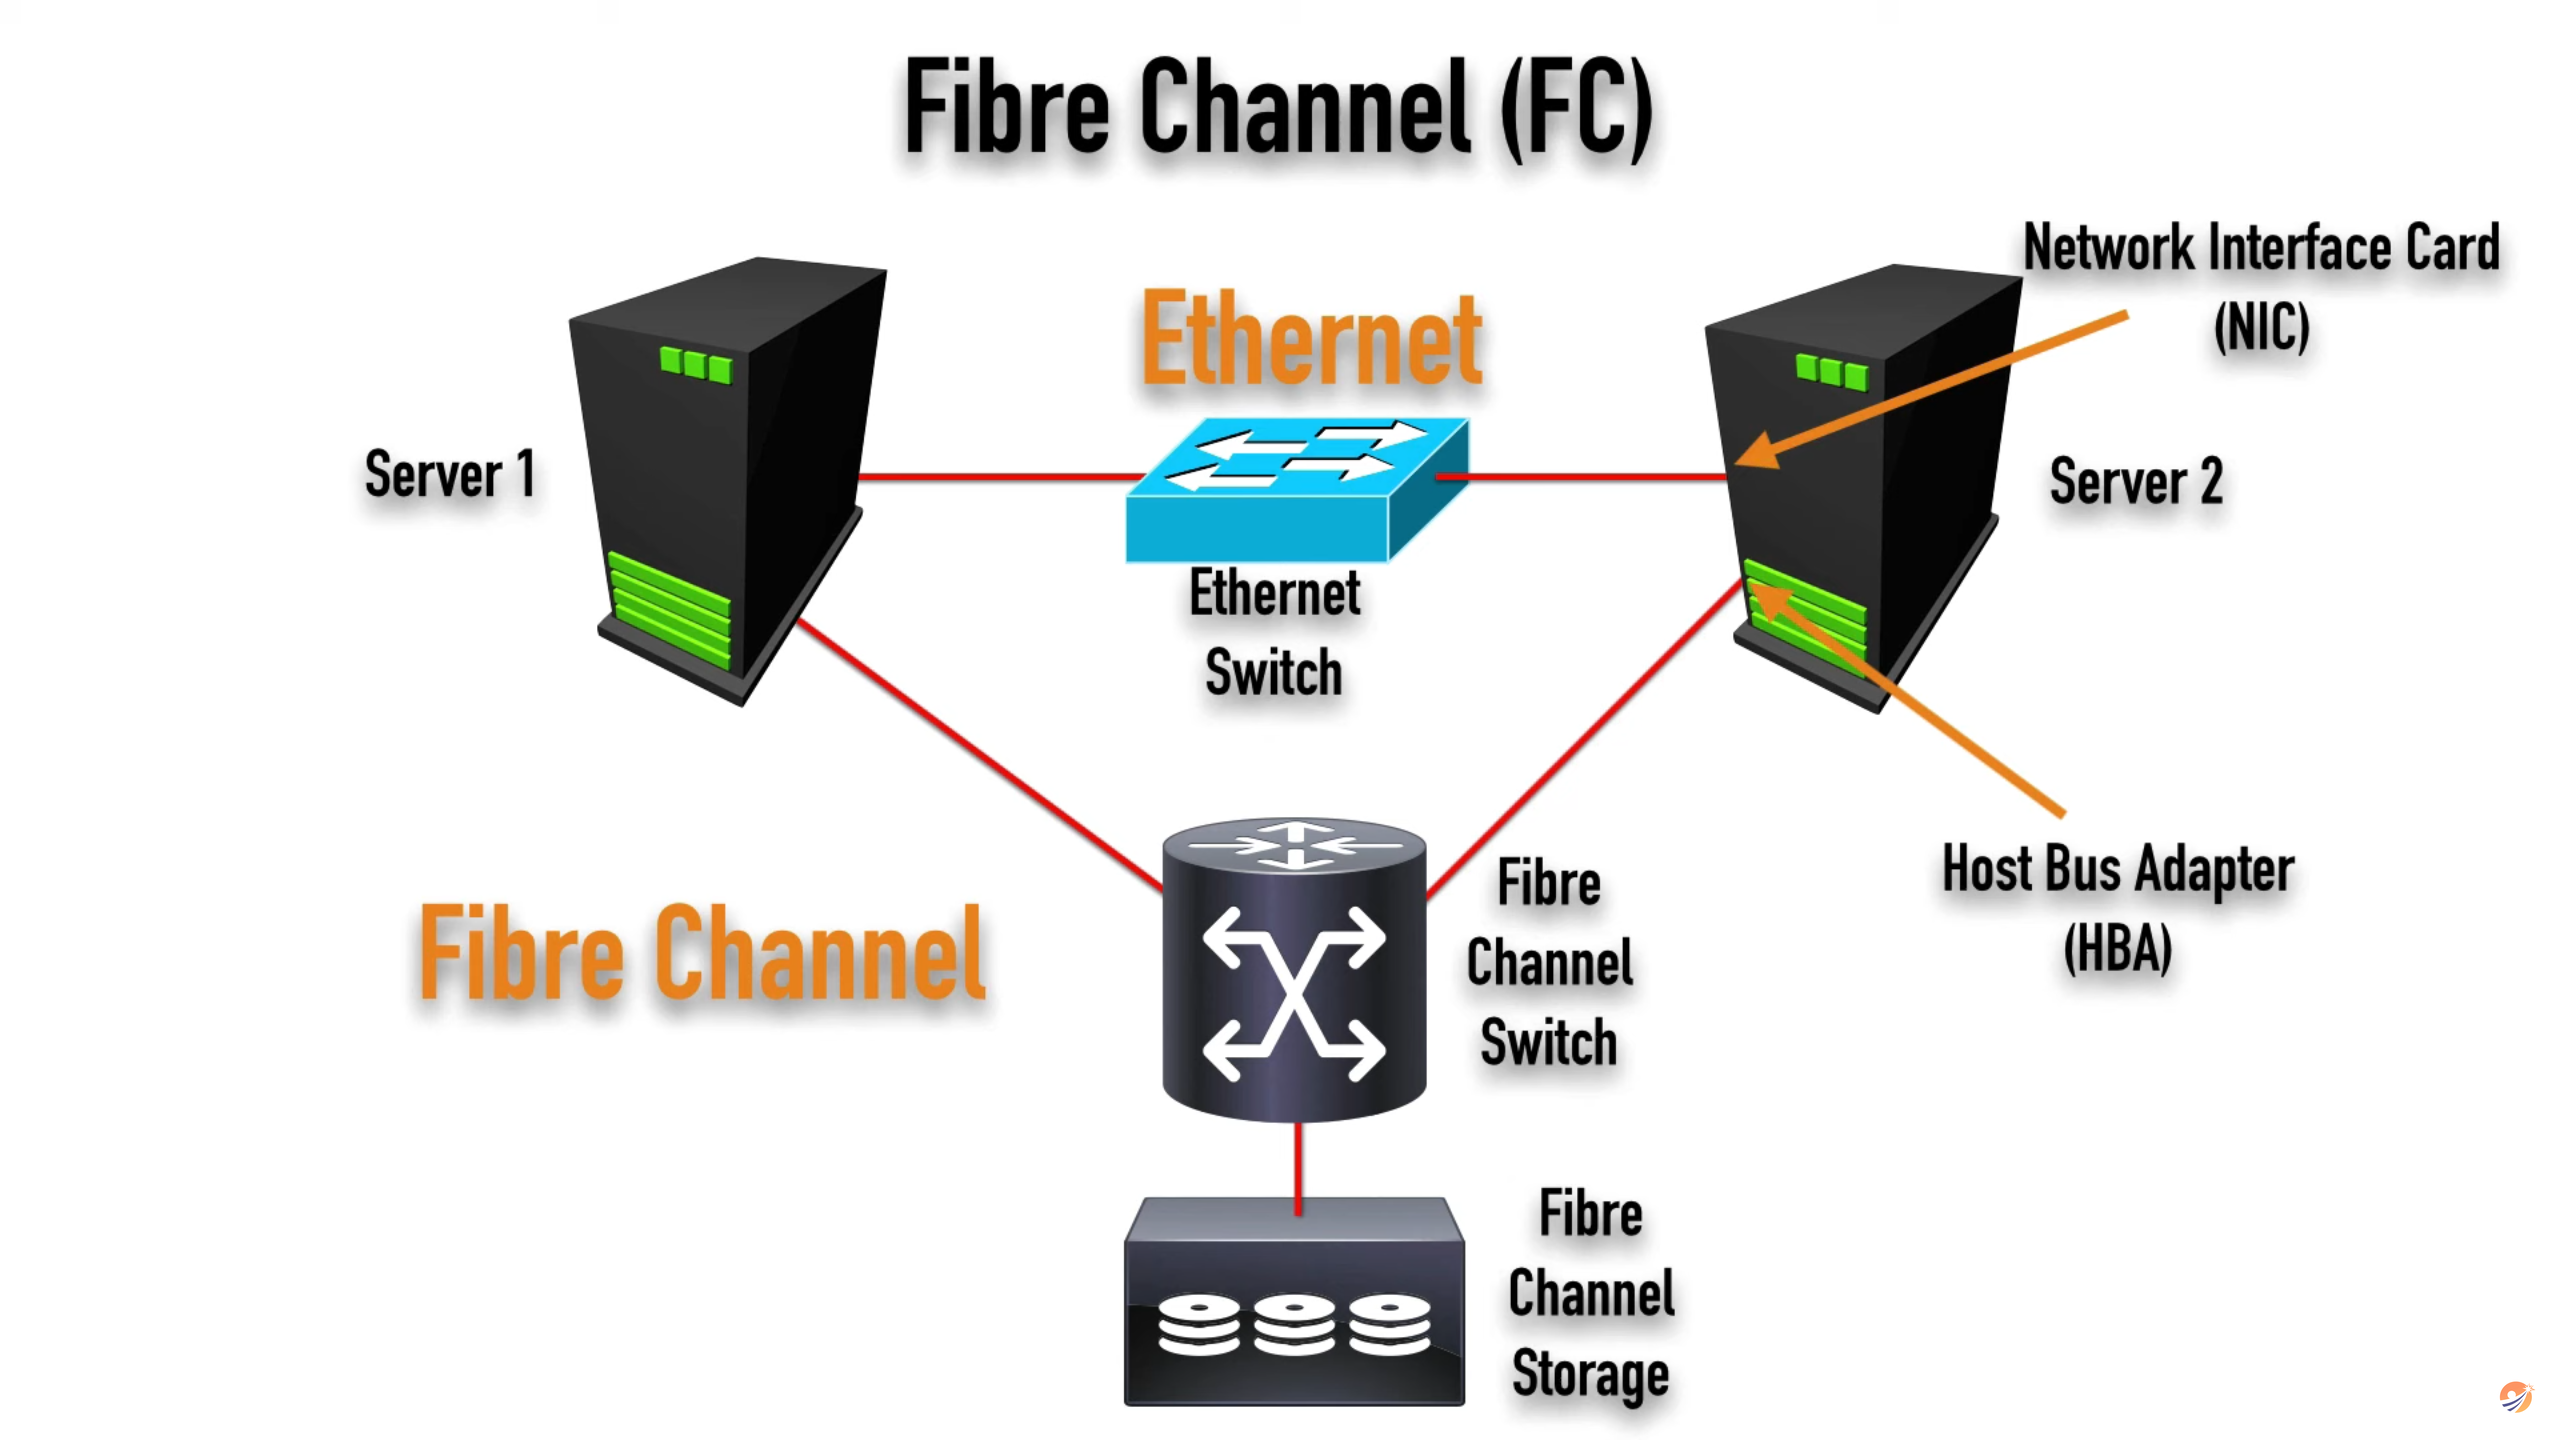
\includegraphics[width=0.32\columnwidth]{images/storage_fabric1.png}
   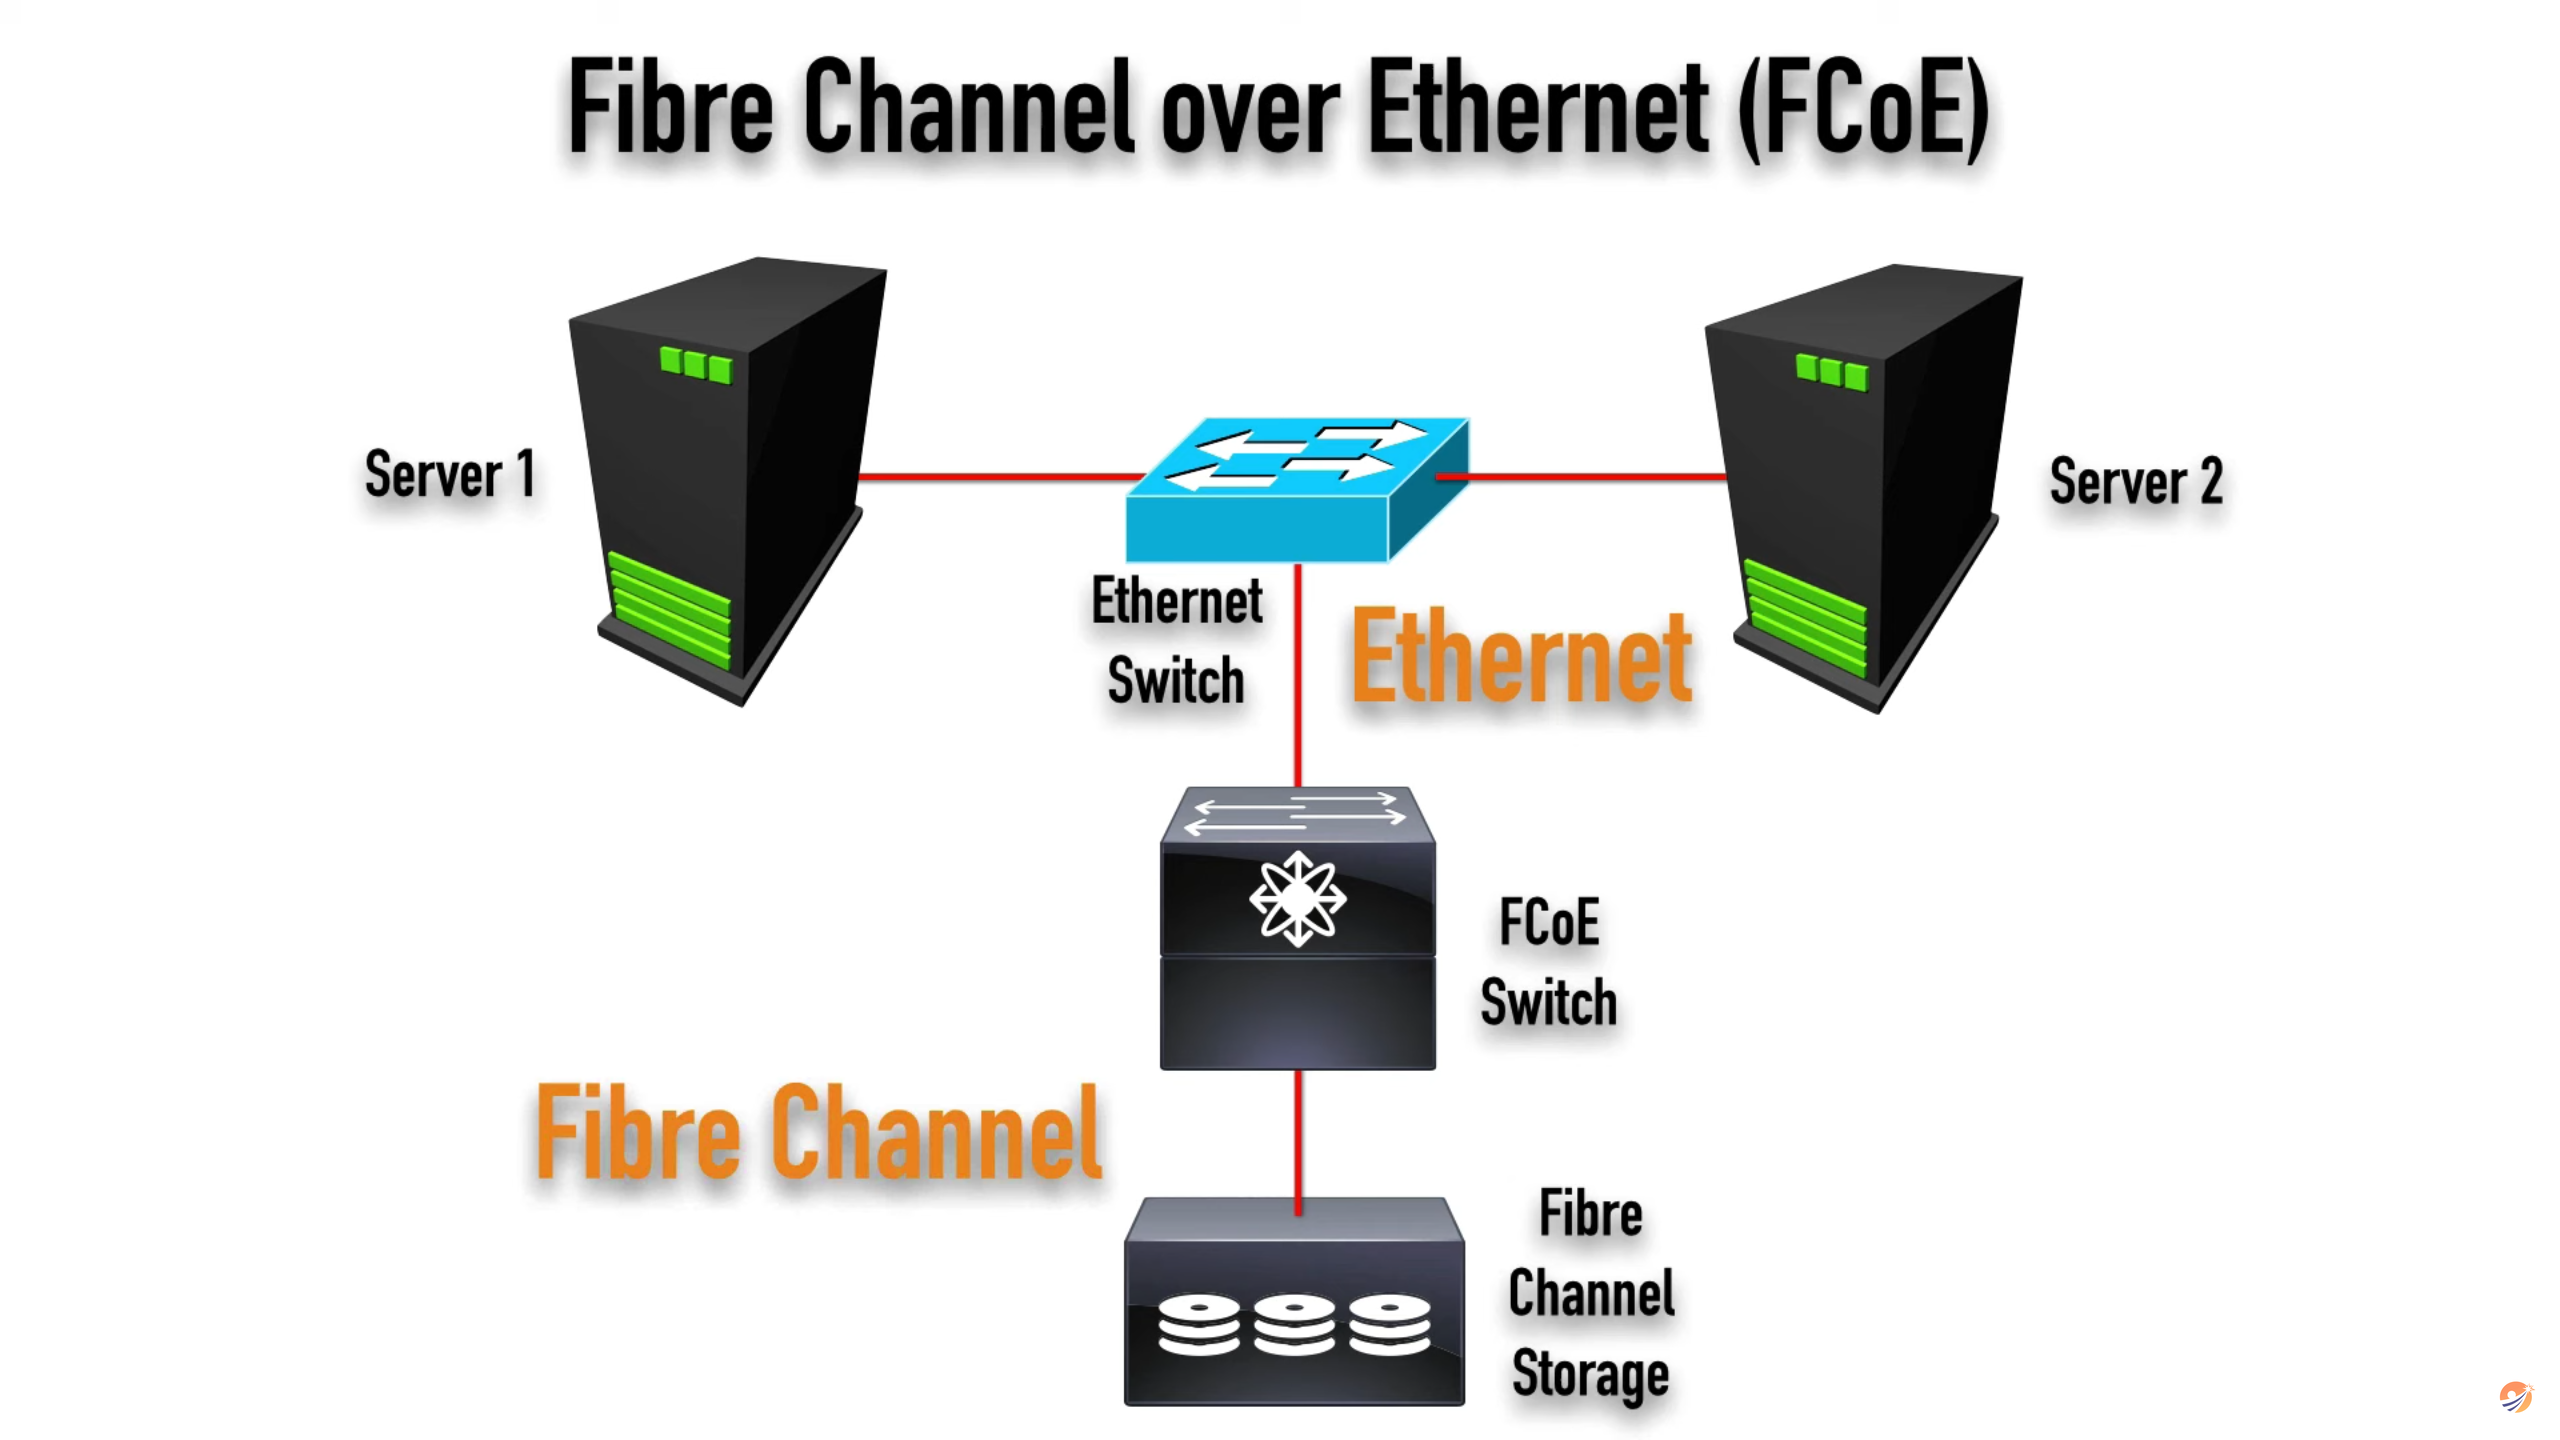
\includegraphics[width=0.32\columnwidth]{images/storage_fabric2.png}
   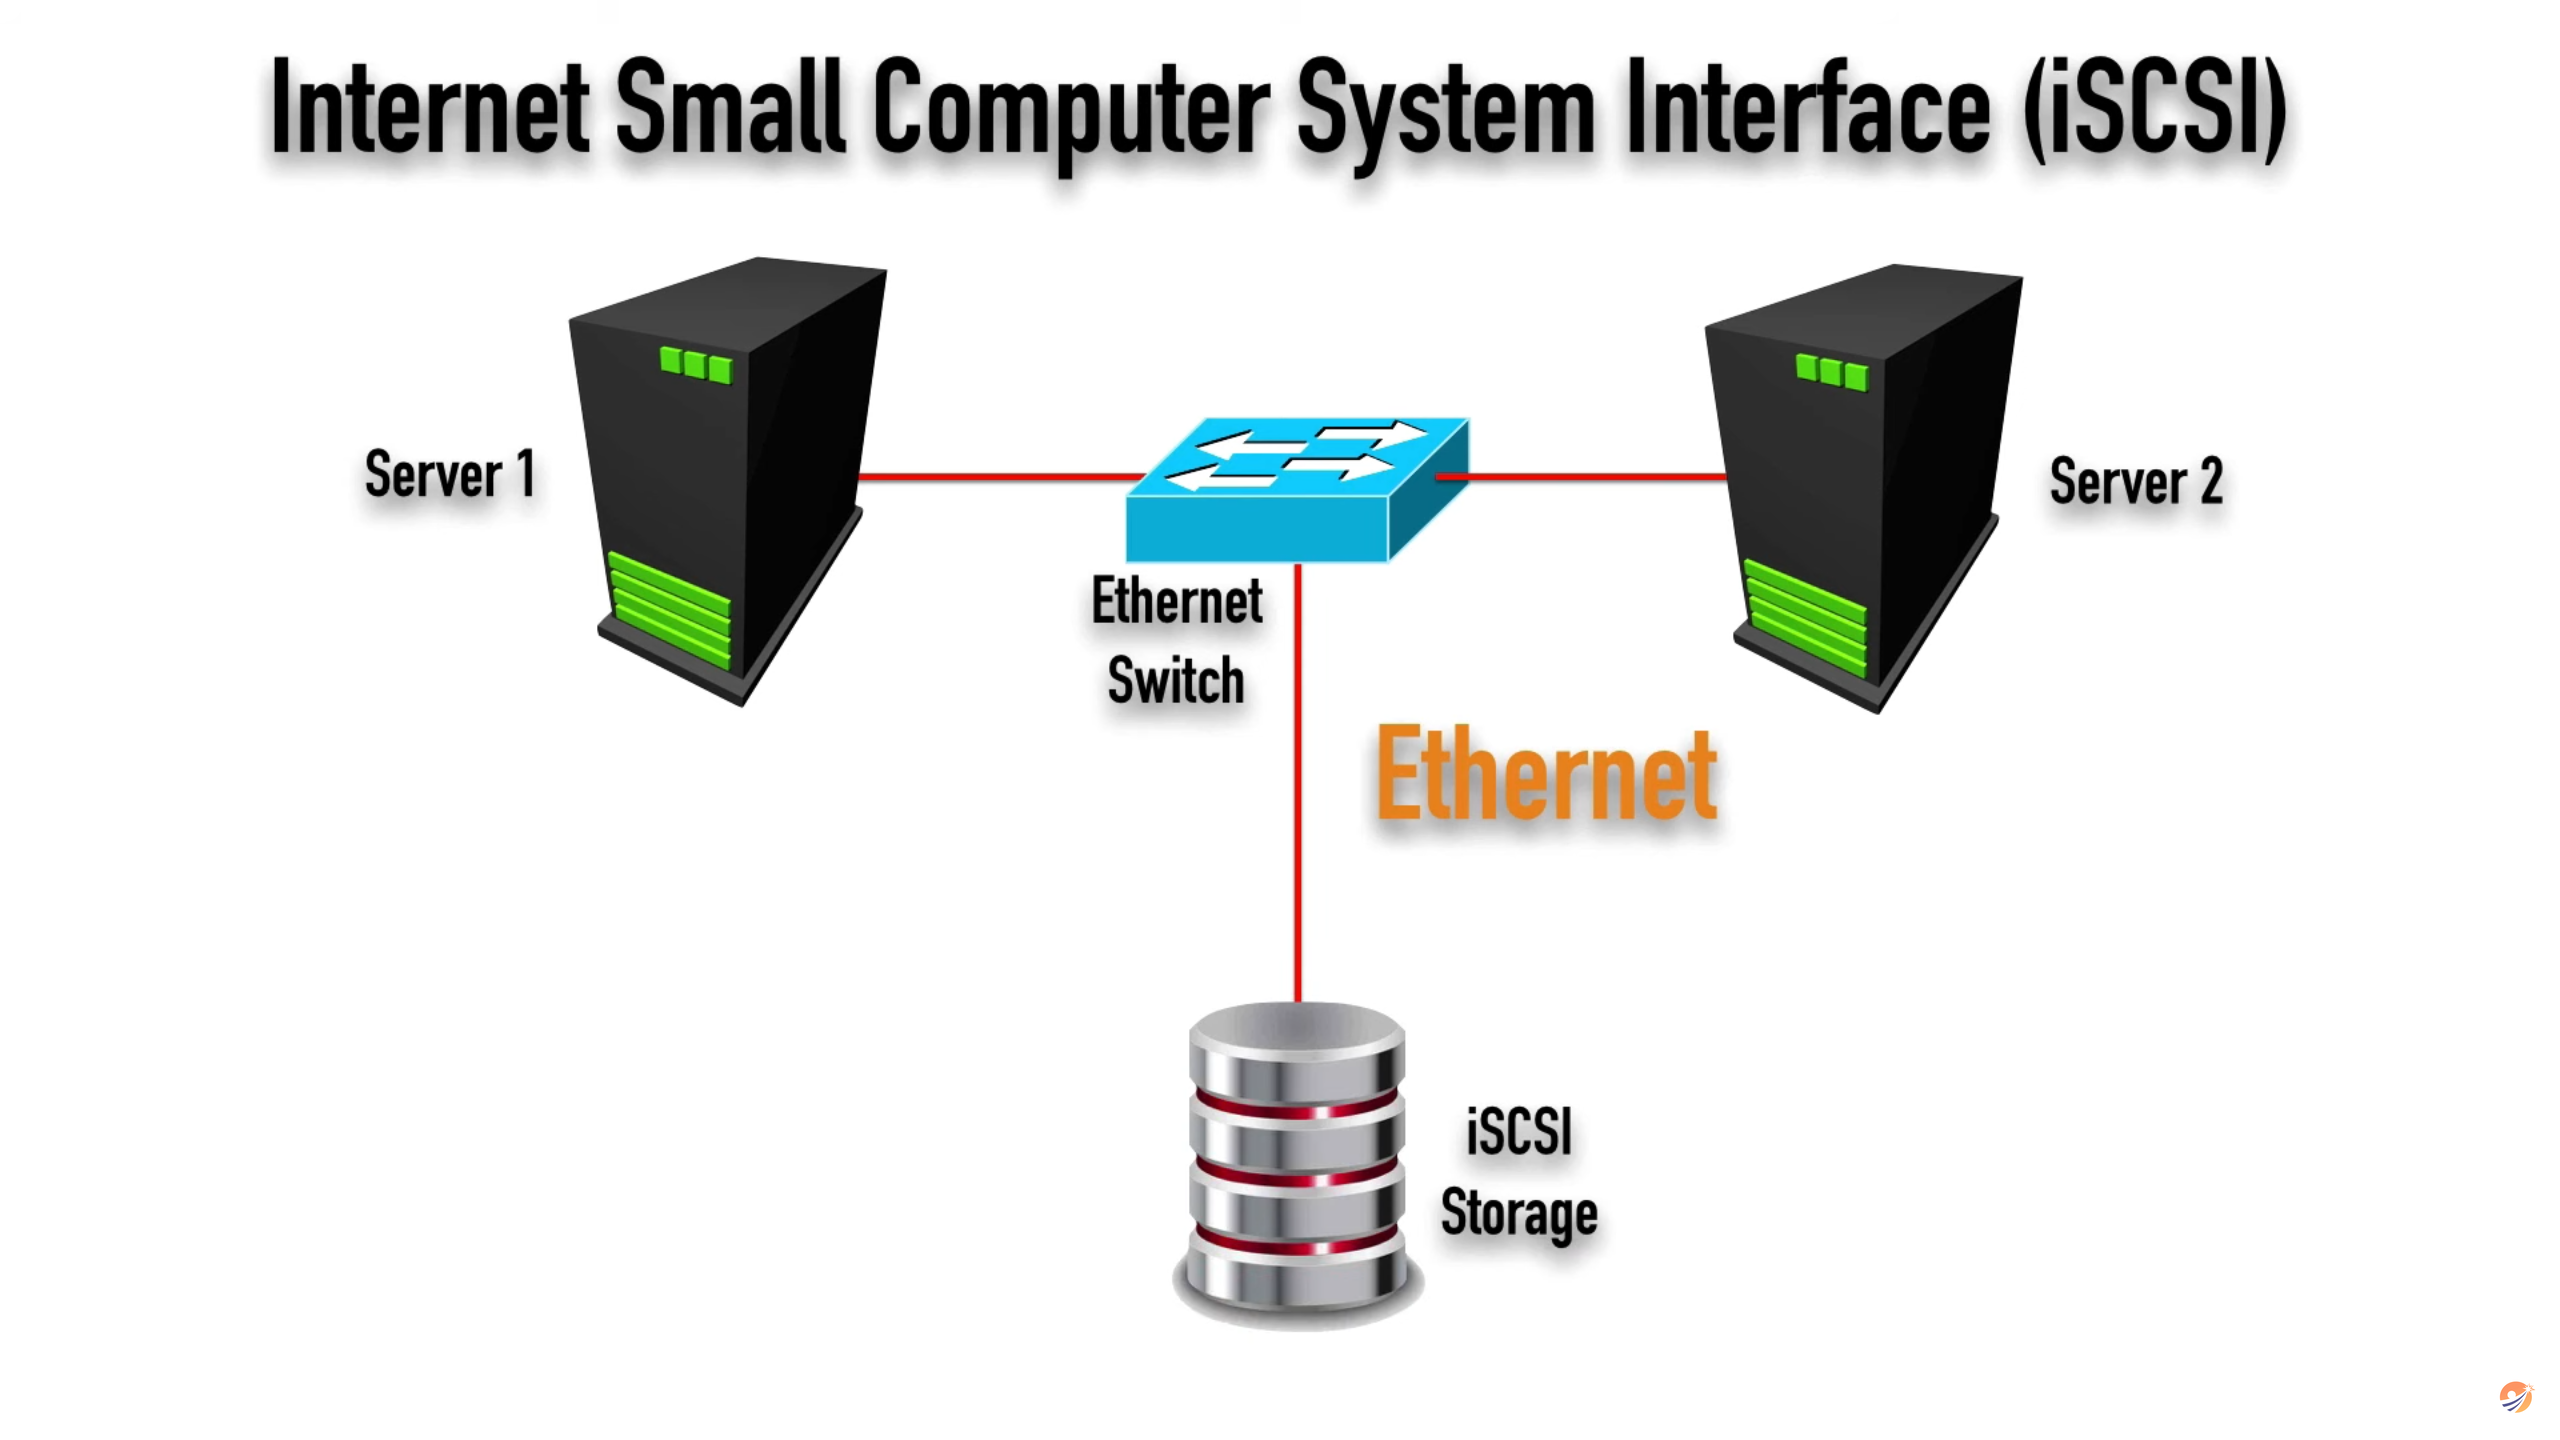
\includegraphics[width=0.32\columnwidth]{images/storage_fabric3.png}
   \caption{These are three possible configurations for the storage fabric, the first being the most performant, and the third being the cheapest.
   Note that in the second picture the first link is Ethernet and the second is Fibre Channel.}
   \label{fig:storage_fabric}
\end{figure}
Note that the image may me misleading, since there may be multiple FC switches (as partially depicted in Fig. \ref{fig:fibrechannel}) and multiple storage racks.
   
\subsection{Bus, controller and some numbers}
A bus is a component to whom multiple devices may be attached. It has a clock and some lanes, 16 in the case of PCI, each one providing almost 1GB bandwidth, summing up to $\sim 15GB$: 4 drives are enough to saturate a full PCI bus, or a 100Gbit link ($12.5GB/s$).;
in fact an NVMe SSD has a bandwidth of 3.5GB/s, hence $3.5\times 4 = 14GB/s \simeq 15GB/s$.\\
NVMe is often used in the lower memory tier of the RAM: its speed is only one order of magnitude less than RAM, but can provide high capacity without any problem.
It may represent a valid super-fast cache level for the RAM and hence started being associated in one single level to implement a big RAM tier, in a totally transparent way for the system.

Since the software latency in disk IOs is 5 microseconds more or less,
TCP/IP software introduces also a latency of 70-80 microseconds, the disk is
no more a problem. Indeed, the problem is now the network, not only for the
latency, but also for the bandwidth: as stated before 4 NVMe totally saturate a 100 Gbps
link.

\section{Redundancy and backup}
\subsection{Checkpoints}
It's unpractical for a system to go down after 5 months. For this reason it is necessary to have \ul{\textit{checkpoints}, which are points in time where the system can be restored to.} The system can be restored to the last checkpoint, and the data that was written after the checkpoint can be re-applied. This is similar to what happens to applications on smartphones are closed and then re-opened, the application is restored to the last checkpoint.

\subsection{RAID}
\textbf{RAID} stands for \textit{Redundant Array of Independent Disks}. It is a technology that allows to combine multiple disks into a single logical unit, in order to increase the performance, the reliability, or both. There are different levels of RAID, each with different characteristics.

Historically \textit{Redundant Array of Inexpensive Disks}, because it was more common for disks to eventually fail, so RAID was the only countermeasure to this. Today, disks are more reliable, so RAID is used more for performance reasons.

In RAID, \textbf{XOR} is used to calculate the parity of the data. The parity is used to recover the data in case of a disk failure. The parity is calculated by XORing the data of the disks. The parity is stored on a separate disk, called the parity disk. The parity disk is used to recover the data in case of a disk failure.


\section{Network sharing architectures}
Before going into the details of the architectures, it is important to understand the difference between \textbf{protocols} and \textbf{architectures}.\\
\textbf{SMB/CIFS} is a protocol that allows to share files over the network. It is used by Windows, but it is also supported by Linux and MacOS. NFS is a protocol that allows to share files over the network, it is used by Linux and MacOS, but it is also supported by Windows.\\
NFS is faster than SMB, but it is also less secure. SMB is slower than NFS, but it is also more secure.\\
These however are protocols for file sharing, not properly ``architectures''.

\framedt{Capacity and system architecture}{
   When we talk about \textbf{capacity}, there are two measures which we can refer to:
   \begin{enumerate}
      \item \textit{Scale-\textbf{up}}:
      adding more disks to the same server
      \item \textit{Scale-\textbf{out}}:
      adding more servers to the same network
   \end{enumerate}
}

\subsection{File based - NAS}
\textbf{NAS} are devices that are connected to the network, and that are used to store files, providing aggregated capacity. They are used to store files that are accessed by multiple users, and that need to be accessed from multiple devices.
NAS systems have integrated HW and SW component, including CPU, memory, NICs, optimized OS for file serving, file sharing protocols and so on.\\
Typically they exploit SMB/CIFS or NFS protocols, or AFP over optical fiber, and represent a good solution for \textit{document management}.

\subsection{Block based - SAN}
\textbf{SAN} stands for \textit{Storage Area Network}, which enables the creation and assignment (i.e. access and share) of storage volumes to compute systems.\\
The compute OS (or hypervisor) discovers these storage volumes as local drives.
The servers have different NICs (HBA) connected (usually through
fibre channels) to those blocks, which are aggregated volumes.\\
SAN also enables performance optimization of the storage by performing
deduplication (delete sequence of blocks that are equivalent).

\note{HBA stands for \textit{Host Bus Adapter}, and is a device that allows to connect a computer to a storage device. It is used to connect a computer to a storage device, and to allow the computer to access the storage device.}

SAN are a network separate from the LAN, so not affected by its traffic.\\
They usually exploit Fibre Channel or iSCSI (which is not as fast) protocols.

SAN was, before SSDs, one of the datacenter pillars.
Its architecture included a ``head'', an advanced Fibre Channel switch, to which drives were attached, and the head was connected to the network. The head was used to manage the drives, and to allow the servers to access the drives.\\
When SSDs became popular, the head became a bottleneck, because it was not able to keep up with the speed of the SSDs(Recall that 4 SSDs are enough to saturate a 10Gbit link, See Sec. \ref{sec:bandwidth_storage}). 
For this reason, the head may be removed, with the drives connected directly to the servers. This is called \textbf{DAS}, typically uses SCSI protocol, but is not as scalable as SAN.

However with groups of mechanical drives, ---if the data is splitted in a smart way--- it's possible to be faster of a single SSD, since the request will be forwarded in parallel to different drives.

\subsubsection{Protocols}
SANs are classified based on protocols and fabric they support. Some possible configurations can be found in Fig. \ref{fig:storage_fabric} 
Common SAN deployments types are Fibre Channel SAN (FC SAN), Internet Protocol SAN (IP SAN), and Fibre Channel over Ethernet SAN (FCoE SAN), ATA over Ethernet (AoE) and HyperSCSI ().
It can be implemented as some controllers attached to some JBoDS (Just a Bunch of Disks).

\note{While NAS provides both storage and a file system, SAN provides only block-based storage and leaves file system concerns on the “client” side.
However, note that a NAS \textit{can} be part of a SAN network.}


\subsubsection{Pools and LUNs}

\textbf{Storage pools} are used to combine multiple storage devices into a single logical unit, in order to increase performance and reliability. 

The SAN is divided in different Logical Unit Numbers (\textbf{LUN}s), which abstract identity and internal functions of storage devices, and appear as phyisical storage to the compute system.\\
\textbf{Storage LUNs} define a storage partition and are used to assign storage ---a portion of the pool--- to a server, and to allow the server to access the storage, using ACLs.
\nl

In the following section, some LUNs features are listed
\begin{itemize}
   \item 
   Storage \textbf{capacity} of a LUN can be dynamically expanded or reduced
   by means \textbf{virtual storage provisioning}, i.e. present a LUN as if it has more capacity than it actually has, to avoid fragmentatation and then expand it when it is needed.
   \note{e.g. if you assign a 1TB LUN to a server, and then you need to expand the LUN due to lack of space, if you have space next to the already assigned TB you can avoid fragmentation. Besides, if you can put data in only 1TB instead of 2TB (even if you present the volume as if it had 2TB), internal fragmentation may happen only inside that TB, and later on you can expand the volume up to the reserved 2TB.}
   Besides, \ul{available space may \textit{decrease} over time}, mostly due to snapshots (discussed later on).
   \item LUNs may perform \textbf{deduplication} (delete sequence of blocks that are equivalent/redundant, and exploiting indexes to retrieve duplicated data) to optimize storage performance. It is very useful in document-rich file systems, since people tend to copy a document multiple times.
   \item LUNs may perform \textbf{compression} to reduce the size of the data, and to increase the performance. It may be lossy or lossless.  Its major downside is that it is computationally expensive, since the data must decompressed before using it.
   On the other hand, allows to spare bandwidth by sending compressed data, which we know to be critical.\\
   \textit{Searching} in compressed data is not trivial, but there are tools to do it, such as the \href{https://en.wikipedia.org/wiki/FM-index}{\texttt{FM-index}}.
   \item LUNs may create \textbf{snapshots}, \textit{``point-in-time''} copy of current data state, to save the differences between the current state of the data and the previous state of the data. This allows to recover the overwritten data in case of a failure, but it also takes up space.\\
   Snapshots older than a week are usually deleted, since they are not needed anymore.
   
\end{itemize}

\subsubsection{Provisioning and Capacities}
LUNs may be created from\ns
\begin{itemize}
   \item A \ul{RAID set} (traditional approach); suited for application that require predictable performance
   \item A \ul{storage pool} (modern approach); suited for application that require flexibility and scalability, and that tolerate performance variations.
\end{itemize}

Both of these approaches have different capacities:\ns
\begin{itemize}
   \item Row capacity: the total capacity of the LUN, limited by the physical capacity of the storage devices
   \item Usable capacity: the capacity that is available to the server, limited by data structures needed to allocate the file system.
   \item Provisioned capacity: the capacity that you present to the server. May be more than the usable capacity, obtaining overprovisioning. 
\end{itemize}

\subsection{Object based - S3}
\textbf{S3} stands for \textit{Simple Storage Service}, and is a service that is used to store file data in the form of objects based on the content and other attributes of the data rather than the name and location of the file.
The additional metadata (size, date, ownership\dots) or attributes (retention, access pattern\dots) enable optimized search, retention and deletion of objects.\\
A flat, non-hierarchical address space to store data provides the flexibility to \textit{scale massively}.\\
\ul{S3 is leveraged to provide Storage as Service.}

\subsection{Big Data - HDFS}
\textbf{HDFS} stands for \textit{Hadoop Distributed File System}, and is a distributed file system that is used to store large amounts of data across multiple servers.
A \texttt{map/reduce} algorithm is applied on the data, and then results are collected and summarized.\\
It exploits good forms of parallelism to run efficiently the algorithm

\subsection{Unified - Unified Storage}
\textbf{Unified Storage} or multi-protocol storage has emerged as solution that consolidates block, file and object storage into a single storage platform. It supports multiple protocols, such as NFS, SMB, iSCSI, FC, REST and SOAP.

\framedt{iSCSI and its death}{
   SCSI (Small Computer System Interface) was invented in 1979 for chaining drives
   through a bus (used for e.g. in fibre channels). The controller was so smart
   to allow the the drive to share the flat cable as a bus.\\
   Over the time some variants were invented, but the basic idea is the same.
   One example is iSCSI: \textit{Internet Small Computer Systems Interface}, an IP-based storage networking standard for linking data storage facilities.
   It provides block-level access to storage devices by carrying SCSI commands over a TCP/IP network. The protocol died when SSD were introduced, since the latency was too high when communicating over the network.

   The key idea behind SCSI was for \ul{mutiple drives to share the same physical flat cable}.\\
   It had been ``deprecated'' in favor of \texttt{NVMe}, but it is still used today, because it is very reliable.
}
\subsection{Synchronization Software and its Price}
The ``storage guy'' must ensure that there is no condition under which can happen data loss, because it is never an option. It is also important to have powerful \textbf{synchronization algorithms}, which must allow data to be copied and synchronized in multiple locations without disrupting performance and handling concurrency;
such software is typically \textit{costful}.

It is difficult nowdays to establish what is the ``right'' price for software. The shift from highly specialized and costful hardware to general hardware-plus-software, gave the software, which still is a non-physical entity, increasingly more value, perhaps even too much.


\section{Hyperconverged Infrastructure}
SAN started to create a sensible bottleneck, so designers started to ``move drives towards the servers''.
\textbf{DAS} stands for \textit{Direct Attached Storage}, and is a technology that allows to connect multiple storage devices to a single server, in order to increase the performance, the reliability, or both.
The limitations is that you can only attach up to 2 or 3 drives to a server.

An idea came out to use the servers' internal drive to build a Storage Area Network, and this is called \textbf{VSAN}.

\subsection{HCI solutions}
\textbf{HCI} stands for \textit{Hyperconverged Infrastructure}, and is a technology that allows to combine multiple servers into a single logical unit, in order to increase the performance, the reliability, or both. 
The idea was born to allow a scale-out architecture, where you can add more servers to the network.

\begin{center}
   \ul{\textit{``Adding servers adds capacity''}}
\end{center}

The \textbf{Hypervisor} is the software that allows to run multiple virtual machines on a single server. There should be some locality between the VM and the storage, because the VM should be able to access the storage quickly.\\
The \textit{controller VM} (one per host) implements the storage abstraction and the logical moving of data.
\texttt{read} operations are always performed locally on local drives; \texttt{write} operations instead sometimes require to retrieve a remote piece of data.
A copy on the local server storage is kept, but the server needs to wait for the acknowledgment of the remote server in order to keep updated replicas of written data in other nodes.

As mentioned in the section dedicated to HCI and networking Sec. \ref{sec:HCI_network}, new server are automatically added to the network seamlessly integrating with the pre-existing HCI cluster.
The same applies to the storage, which is automatically added to the pool, and local replicas of data are built.

\subsubsection{VM Live Migration}
Live Migration of VMs is a technique that allows to move a VM from one server to another server, without interrupting the service. 
When it happens over SAN there's no need to copy storage to the new server, since the storage is shared and accessed through the network.
The case of HCI is similar since the storage is mostly shared, but there are also the above mentioned local copies of data, which may need to be updated. 

\subsection*{Riak and Acropolis}
Riak is a distributed database that is used to store data in multiple locations. 
The same applies to Acropolis, which is a distributed storage system.

Recently it has been recognized that \ul{using general purpose hardware is no longer a feasible option.}

\section{SDS - Software Defined Storage}
\textbf{SDS} \textit{Software Defined Storage} refers to software for policy-based provisioning and management of data storage independently from the underlying hardware.
Such software is more costful than the hardware it is running on, since it also optizimes the drives, not simply managing them.\\
SDS exploits object-based storage architecture and DHTs to provide storage services.
\chapter{Attacks}
% \section*{3 - Ottobre}
\section{Attacks and Vulnerabilities}
Following the discovery of a vulnerability $v$ there's an analysis to evaluate which attacks are enabled by $v$.
\textbf{Attacks} can be described as a set of attributes:
\begin{enumerate}
    \item Precondition
    \item Postcondition
    \item Success Probability
    \item Know how, abilities, tools required
    \item Noise = Probability of being discovered
    \item Automated/Potentially automatable/manual
    \item Local/Remote
    \item Actions to implement attack\footnote{See following Section on attack taxonomy}
\end{enumerate}
Even though some attack evaluation proposals map to each attribute a number and combine them into a value,
such evaluations do not consider that \textbf{risk} resides in \textit{intrusions}, not individual attacks, because they have a considerable impact on the system, and keep in mind that are composed by:
\begin{itemize}
    \item Exploration and information collection
    \item Persistence
    \item Attack \textit{chain} for privilege escalation
\end{itemize}

\section{Attack Classification}
\label{sec:attack_taxonomy}
The actions need to implement an attack may be used to define a \textbf{taxonomy} of attacks:
\begin{enumerate}
    \item buffer/stack/heap overflow
    \item \textit{sniffing} $\rightarrow$ Illegal access to info in travel
    \item \textit{replay attack} $\rightarrow$ Repeated exchange of legal messages 
    \item \textit{Interface attack} $\rightarrow$ Illegal order in the invocation of API functions
    \item \textit{Man-in-the-middle} $\rightarrow$ Interception and manipulation of info in travel
    \item Diversion of an information flow
    \item \textit{Race-condition} $\rightarrow$ Time-to-use time-to-check
    \item \textit{Cross site scripting} $\rightarrow$  XSS
    \item SQL injection
    \item \textit{Bell-Lapadula policy} $\rightarrow$ Covert channel 
    \item Masquerading as
    \begin{itemize}
        \item user
        \item machine (\textit{IP/DNS spoofing, Cache poisoning}
        \item connection (\textit{connection stealing/insertion})
    \end{itemize}
\end{enumerate}

\section{Examining attacks}
\subsection*{Replay attack}
Suppose a user asks the bank to transfer some money to $Y$ account with an $M$ message.
$Y$ may sniff and record $M$, and before the secure channel $S$ gets deleted, $Y$ sends $M$ several times.\\
Note that the attack may work even if encryption is used.

\subsection*{Man-in-the-middle}
If $A$ and $B$ communicate, $E$ may pose itself in the middle, acting as if it were $B$ to $A$ and $A$ to $B$.
Such attack is possible when no authentication is required.

\subsection*{XSS}
A website allows users to upload contents to be later (possibly) downloaded by users.
Thus a malicious user may upload hidden scripts to damage or steal information from the user who download their content.
To avoid this the website must check the content uploaded by users.\\
A well known attack of this type targeted BBC.

\subsection*{SQL Injection}
An input may insert a malicious query (i.e. \lstinline[language=SQL]{DROP TABLE USERS}) in a credentials field.
The best way to avoid this is to whitelist using RegEx.

\subsection*{Cryptography attacks}
These are a category on their own, there are many types, with different variations and features.

\subsection*{Side-channel attacks}
Any attack that measures some physical value to discover an encryption key.
Currently it is popular due to the capabilities of machine learning in exploiting large number of pairs to deduce a function.\\
Such measures may be:
\begin{itemize}
    \item Electromagnetic emissions
    \item Energy consumption
    \item Execution time to discover inner status
    \item Execetion time to discover cache usage and prediction mechanisms.
\end{itemize}

\subsection*{Virtual Machines \& Blue Pill}
Cyber system may be composed of many virtual machines onion-like organized.
Thus, attacking a low-level VM may grant access rights to higher ones.\\
Besides, an attacker may insert a new VM in the hierarchy:
this is called \textit{Blue Pill} attack, it's hard to discover and has a high impact.
A new VM may return to higher VMs fake information on the status of the underlying machines and/or send malicious commands to the underlying machines.\\
\texttt{Stuxnet} was a malware which used to send commands to uranium enrichment centrifuges to destroy them, and meanwhile told the operator that everything was going well.  

\chapter{Cloud computing}
\section*{19 - Ottobre}
Powerful hardware and high-speed networking have made room for the development of cloud computing.
\textbf{Cloud computing} allows virtual resources accessible \textbf{on demand},
and provides many advantages against the standard old-style scaling methods i.e. buying resources.
\begin{itemize}
   \item \textit{Scalability}
   \item \textit{Elasticity}
   \item \textit{Resilience}
   \item \textit{Cost}
\end{itemize}

\section{Virtualization and Containers}
\begin{paracol}{2}
   Virtual machines on a single physical machine are managed by hypervisor
   \begin{table}[!htbp]
      \centering
      \begin{tabular}{|cc|}
         \hline
         App A & App B\\
         bins/libs & bins/libs\\
         Guest OS & Guest OS\\
         \midrule
         \multicolumn{2}{|c|}{\textbf{Hypervisor}}\\
         \hline
         \multicolumn{2}{|c|}{Host OS}\\
         \hline
         \multicolumn{2}{|c|}{Hardware}\\
         \hline
      \end{tabular}
   
   \end{table}

   \vspace{\fill}
   \switchcolumn

   Containers instead exclude one layer of abstraction, saving up a lot of resources
   \vspace{\fill}
   \begin{table}[!htbp]
      \centering
      \begin{tabular}{|cc|}
         \hline
         App A & App B\\
         bins/libs & bins/libs\\
         \midrule
         \multicolumn{2}{|c|}{\textbf{Container Manager}}\\
         \hline
         \multicolumn{2}{|c|}{Host OS}\\
         \hline
         \multicolumn{2}{|c|}{Hardware}\\
         \hline
      \end{tabular}
   \end{table}

   \vspace{\fill}
\end{paracol}

\section{Docker}
Docker exploits container-based virtualization to run multiple isolated guest instances on the same SO.
Software is packaged into \textbf{images} which are read-only templates to instantiate and run containers.
External \textbf{volumes} can be mounted to ensure data persistance when used by multiple containers or by the host machine.

It is possible to \textbf{stack} multiple docker \textit{images},
and if desired create a new image as a result of stacking other ones.
\chapter{Containers}
\label{chap:containers}

\ul{A VM is better than a process because it provides \textbf{isolation}}:
a typical problem in cybersec is that if an attacker cracks a process, he may access the whole system;
with a VM, the attacker can only access the VM, not the host.
However, a VM introduces overhead due both to the hypervisor and to the OS (cache, kernel, storage management\dots).

\note{The idea is to tell a process that a process that its root is a subdirectory of the host's root, resulting in a strong isolation.}

\textbf{Docker} provides a \textit{differential filesystem}, which is a filesystem that is a diff of the host's filesystem, an abstraction where the new ``inner'' file system is based on a given one, where the system will only store the differences between the original file system and the new one.

Docker has become the de facto standard for containers, but there are other solutions like \textbf{LXC} (Linux Containers) and \textbf{rkt}.
A Dockerfile contains the information to build a container.

One of the key differences between a VM and a container is that containers \textbf{do \textit{not} have a virtual switch}.
A container uses the same MAC address of the host.\\
Docker containers are processes, and only see a portion of the host's filesystem.

Inside a Dockerfile you may create temporary containers by exploiting multiple images and lastly build the resulting slimmed image.

\section{Upgrading a system}

Typical procedure when a system needs to be updated: create first a snapshot before updating the containers (especially if there are updates related to the database), then update, run back the containers, check if everything works, and then delete the snapshot. If anything goes wrong, the snapshot will help to roll back.

\section{Docker compose}
Docker compose is a tool to define and run multi-container Docker applications. It uses a YAML file to configure the application's services, networks and volumes. With a single command, you can create and start all the services from your configuration.

Kubernetes is a more advanced tool for container orchestration, way more complex than Docker compose, it allows to manage thousands of containers, providing fundamental scalability features.

\section{Docker security}
An attack is to put the machine under heavy workload and observe from the container the performance to infer what other processes may be. This is called \textbf{side channel attack}.

Google has thousands of VMs and each runs a \textit{container for each query}.
\chapter{Cloud}
Cloud came out as a business model, not as a technlogy.
It was needed to handle peak of requests and to allow scalability, without oversizing Infrastructures.
\note{e.g. Amazon needs to handle way more requests on Christmas than on a normal day.}
So, Cloud was a mean to reduce the cost of the ICT infrastructure.

\textbf{Resource pooling} is the key concept of Cloud. It means that the services are provided to users using a multi-tenant model, with physical and virtual resources being dynamically allocated and deallocated according to the demand.\\
Cloud was needed also to provide rapid elasticity, meaning that capabilities may be elastically provisioned and released, in some cases automatically, to scale rapidly outward and inward commensurate with demand. To the customer it means that the capabilities available for provisioning often appear to be unlimited and can be appropriated in any quantity at any time.

Benefits of Cloud:
\begin{itemize}
   \item \textbf{Business agility}
   \begin{itemize}
      \item Quick resource provisioning
      \item Facilitates innovation
      \item Reduces time to market
   \end{itemize}
   \item \textbf{Reduces IT costs}
   \begin{itemize}
      \item Reduces up-front capital expenditure (CAPEX)
      \item Improves resource utilization
      \item Reduces operational expenditure (OPEX)
   \end{itemize}
   \item \textbf{High availability}
   \begin{itemize}
      \item Ensure resource availability based on customer's requirements
      \note{In RAI, prof. Cisternino experienced people complaining because their servers' CPUs were running at 98\% of their capability, and they wanted to exploit also the remaining 2\%, because ``they paid for it''.}
      \item Enables fault tolerance
      \note{Recall active-active, active-passive, etc. configurations.}
   \end{itemize}
   \item \textbf{Business continuity}
   \item \textbf{Flexible Scaling}
   \item \textbf{Flexibility of Access}
   \item \textbf{Application Dev and Testing}
   \item \textbf{Simplified infrastructure management}
   \item \textbf{Increased collaboration}
   \item \textbf{Masked complexity}
\end{itemize}
Cloud has the magic power of decoupling the software from the hardware.

Disadvantages of Cloud:
\begin{itemize}
   \item Vendor lock-in
   \item Privacy
   \item Your software depends on someone else
   \item Legislation is complicated
   \note{In EU public administration data, must be stored in the EU.}
   \item \dots TODO
\end{itemize}

\section{Cloud Service Models}
\begin{itemize}
   \item \textbf{IaaS} (Infrastructure as a Service)
   \begin{itemize}
      \item Provides virtualized computing resources over the Internet
      \item Examples: Amazon EC2, Google Compute Engine, Microsoft Azure
   \end{itemize}
   \item \textbf{PaaS} (Platform as a Service)
   \begin{itemize}
      \item Provides a platform allowing customers to develop, run, and manage applications without the complexity of building and maintaining the infrastructure
      \item Examples: Google App Engine, Microsoft Azure, Heroku
   \end{itemize}
   \item \textbf{SaaS} (Software as a Service)
   \begin{itemize}
      \item Provides software applications over the Internet
      \item Examples: Google Apps, Microsoft Office 365, Salesforce
   \end{itemize}

\section{Cloud Deployment Models}
\begin{itemize}
   \item \textbf{Public Cloud}
   \begin{itemize}
      \item Owned and operated by third-party cloud service providers
      \item Deliver computing resources over the Internet
      \item Examples: Amazon Web Services (AWS), Microsoft Azure, Google Cloud Platform
   \end{itemize}
   \note{It does \textbf{not} mean that the data is public. It means that the cloud services are accessible to the public.}
   \item \textbf{Private Cloud}
   \begin{itemize}
      \item Operated solely for a single organization
      \item Managed by the organization or a third party
      \item \textit{On-premise} or \textit{off-premise}
   \end{itemize}
   \note{It does \textbf{not} mean that the data is private. It means that the cloud services are accessible only to the organization e.g. \textit{UniPi}.}
   \item \textbf{Hybrid Cloud}
   \begin{itemize}
      \item Composition of two or more clouds (private, community, or public) that remain unique entities but are bound together, and resources may be moved from one cloud to another (with some performance cost obviously) 
      \item By standardized or proprietary technology that enables data and application portability
   \end{itemize}
   \item \textbf{Community Cloud}
   \begin{itemize}
      \item Shared infrastructure for specific community
      \item Managed by organizations or third party
      \item On-premises or off-premises
   \end{itemize}
\chapter{Deception with Honeypots}
A \textbf{honeypot} is a system designed exclusively to be attacked an to \textbf{collect information} about the attacker and its tactics, techniques and procedures;
the other focus of an honeypot is also to possibly slow down an attack to a system by \textbf{diverting} it on itself.

The scaled version of a honeypot, is a \textbf{honeynet},
which is an entire network attached to a real system designed to be targeted instead of the main system.

\subsection{Classification}
\begin{enumerate}
   \item \textbf{Interaction}-based
   \begin{enumerate}
      \item \textit{Low} - e.g. simple port listener
      \item \textit{Medium} - emulation of a network service that analyzes the inputs and returns some replies similar to those the real service would return.
      \begin{itemize}
         \item Simulates just some \textbf{features} of the service
         \item Easy to implement, \textbf{low risk}
         \item Can collect a low amount of information
         \item Tools $\longrightarrow$ OS + Honeyd
      \end{itemize}
      \item \textit{High} - built around real services that run on real machines to fool the attacker
      \note{realistic but dangerous due to the large amount of vulnerable software}
      \begin{itemize}
         \item Simulates \textbf{all features} of the service and of the underlyng OS
         \item The attacker may fully compromise and control it
         \item \textbf{High risk}
         \item A larger amount of information
         \item Tools $\longrightarrow$ Honeynet.
      \end{itemize}
   \end{enumerate}
   
   \item \textbf{Implementation}-based
   \begin{enumerate}
      \item \textit{Virtual}
      \item \textit{Physical}
   \end{enumerate}
   
   \item \textbf{Goal}-based
   \begin{enumerate}
      \item Production
      \item Research on attacker behaviour
   \end{enumerate}
\end{enumerate}

\section{Honeyd}
\textbf{Honeyd} is a daemon which creates virtual nodes in a network.
It is highly configurable and is able to reproduce even large and complex networks;
besides it can integrate with virtual and physical real-existing networks.\\
\textbf{Honeyd} provides many features, we can list some of the main ones:
\begin{itemize}
   \item It detects illegal activities in a network by monitoring the IP addresses that are not within a \textbf{range} named \textit{"dark space"}.
   Any attempt of connection to or from the \textit{dark space} is assumed to be an attack or a vulnerability scan.
   \item It monitors activities related to TCP and UDP ports and ICMP traffic.
   \item It can emulate network services using script in Perl, shell or other way of interacting with the attacker.
\end{itemize}

\subsection{Architecture}
\begin{itemize}
   \item \textit{Configuration database} -
   Queried to discover the model paired with the destination IP address
   \item \textit{Packet dispatcher} -
   analyzes input packets and checks correctness and integrity.
   Anything different from TCP, UDP and ICMP gets \textit{discarded}.
   \item \textit{Protocol manager} -

   \item \textit{Personality engine} -
   computes a reply packet and updates it to guarantee coherence with the OS that the destination is expected to use
   \item \textit{Optional routing component} -
   allows the routing of a packet to a real application
\end{itemize}

\subsection{Research results}
\textbf{Honeypot}s provided an important amount of data to perform research on.
Many statistics have been computed to produce estimations and interesting results,
a \textit{\textbf{UniPi} student presented a thesis on the topic} \smiley.
\note{Honeypot thesis available in the \href{https://elearning.di.unipi.it/mod/resource/view.php?id=18233}{web page of the course}}
\chapter{Partitioning}

\textbf{Partitioning} becomes necessary when dealing with \textbf{large data sets} and high \textbf{query throughput}. It is a technique that divides a large data set into smaller, more manageable parts. This is done to improve the performance of the system. Partitioning can be done in various ways, such as horizontal partitioning, vertical partitioning, and functional partitioning. In this chapter, we will discuss the different types of partitioning and their benefits.

``Partition'' is the most common term, but it may vary depending on the technology:
\begin{itemize}
   \item \textbf{Shard} in MongoDB, Elasticsearch, and Cassandra.
   \item \textbf{Region} in HBase.
   \item \textbf{VBucket} in Couchbase.
   \item \textbf{Tablet} in Bigtable.
   \item \textbf{VNode} in Riak and Cassandra.	
\end{itemize} 

\section{Partitioning concepts}
First, partitions must be \textbf{defined}, in the sense that each piece of data must be assigned to a partition. This can be done in various ways, such as hashing, range partitioning, or list partitioning.

Then, each partition should have its own \textbf{characteristics}, i.e. should support a known set of operations, since it acts as a small per se database.

Clearly, different partitions may reside on different nodes, enabling scalability.


\subsection{Combining partitioning with replication}

\begin{paracol}{2}
   \colfill
   Partitioning can be combined with replication to improve the performance and reliability of the system. Replication is the process of creating multiple copies of the data and storing them on different nodes. This ensures that the data is available even if one of the nodes fails. \ul{By combining partitioning with replication, you can achieve high availability and fault tolerance.}
   \colfill
   
   \switchcolumn

   \begin{figure}[htbp]
      \centering
      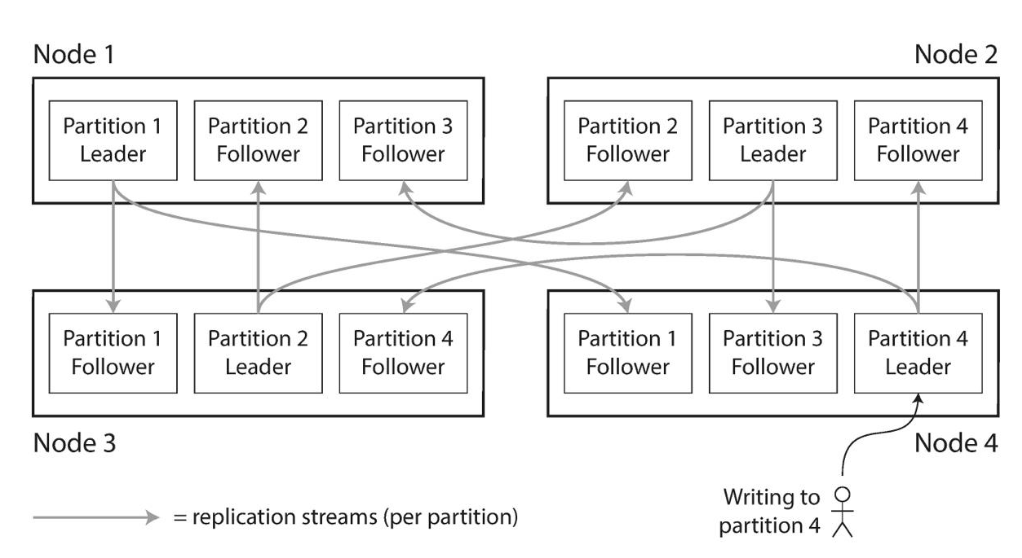
\includegraphics[width=0.95\columnwidth]{images/11/leader_follower.png}
      \caption{Leader-follower model}
      \label{fig:11/leader_follower}
   \end{figure}
\end{paracol}

This can be achieved in various ways:
\begin{enumerate}
   \item Node Storage of Multiple Partitions
   \begin{itemize}
      \item Nodes can store more than one partition, and \ul{each partition can be stored on multiple nodes}.
   \end{itemize}
   \item \textbf{Leader} and \textbf{Follower} assignment
   \begin{itemize}
      \item Each node stores a partition, and one of the nodes is designated as the leader. The leader is responsible for handling all write operations, while the followers replicate the data from the leader.
   \end{itemize}
   \item Replication and Partitioning
   \begin{itemize}
      \item The two techniques are enforced independently.
   \end{itemize}
\end{enumerate}

The Goal of partitioning is to spread data and query load \textbf{evenly} among the nodes.
Unfair partitioning can lead to \textbf{hot spots}, where some nodes are overloaded while others are underutilized.\\
Randomizing the partitioning function can help to avoid hot spots, but it can also make it difficult to locate data, requiring to query all nodes to get a value.

\subsection{Key-Range Partitioning}
A first improvement might be to provide a range-key assignment allowing to locate data, as it happens in libraries, where books are ordered by author or title.\\
In this way you know the boundaries of where to search. This is very easy to implement and to understand,
however, it is \textit{not} optimal:
\ul{data may \textbf{not} be evenly distributed among the possible keys}.

\section{Avoiding Hot spots}
So with key-range partitioning, the problem is that some keys may be more popular than others due to access patterns, leading to hot spots.\\
In, for instance, a sensor database, all today's writes would end up in the same ``today's partition'', while the rest of the partitions would be idle.
\nl

A solution might be to change-key structure, for instance by adding a prefix to the key, such as the sensor ID, to distribute the data more evenly.

\subsection{Hash partitioning}
A better solution is to use \textbf{hash partitioning}, where a hash function is used to map keys to partitions.\\
However we must be careful because \textbf{inconsistent} hashing can lead to hot spots, as the hash function may not distribute keys evenly.

Note also that hash partitioning is very bad for range queries, as even similar data is spread randomly across the partitions.

\subsubsection{Secondary Indexes}
% Copilot generated
Secondary indexes are a way to avoid hot spots in hash partitioning.\\
The idea is to create a separate index that maps the secondary key to the primary key, and then use the primary key to locate the data.\\
This way, the secondary key is hashed and distributed evenly across the partitions, while the primary key is used to locate the data.


\begin{itemize}
   \item \textbf{Document}-based partitioning (local indexes)
   \begin{itemize}
      \item Each listing has a unique document ID
      \item Database is partitioned based on the document ID
      \item Secondary indexes are on fields like color and make
      \item \ul{\textit{Reading} requires querying all partitions}
   \end{itemize}
   \item \textbf{Term}-based partitioning (global indexes)
   \begin{itemize}
      \item A Global index covers data in all partitions.
      \item Partitioning is based on the term ID, which is not the primary key index.
      \item 
   \end{itemize}
\end{itemize}

\section{Rebalancing}
Rebalancing is the process of moving data between partitions to ensure that the data is evenly distributed among the nodes. This is necessary when the data distribution changes, for example, when new nodes are added to the system or when the data distribution becomes uneven due to hot spots. Rebalancing can be done in various ways, such as automatic rebalancing, manual rebalancing, and dynamic rebalancing.

\framedt{Challenges in rebalancing}{
   \begin{itemize}
      \item Fair load distribution
      \item Continuous operation during rebalancing
      \item Minimizing data movement
   \end{itemize}
}

\subsection{Optimizing rebalancing - Kademlia and P2P recalls}

Assigning keys to nodes computing $h(key) mod \#{nodes} \rightarrow node$ is intuitive but leads to a tremendous amount of data movement when nodes are added or removed, since all modulo values must be recomputed.\\
A better solution is to use a \textbf{distributed hash table} (DHT) such as \textbf{Kademlia} or \textbf{Chord}, which allows to find the node responsible for a key in $O(\log n)$ steps.

A simple intuition exploited by both Kademlia and Chord is to fix the granularity of the keyspace prior to partitioning.

In other words, having a fixed number of partitions may help to avoid data movement when nodes are added or removed.


\subsection{Dynamic partitioning}
Dynamic partitioning is a technique that allows the system to adapt to changes in the data distribution. This is done by monitoring the data distribution and rebalancing the data when necessary. Dynamic partitioning can be done in various ways, such as automatic rebalancing, manual rebalancing, and dynamic rebalancing.

\begin{itemize}
   \item \textbf{Automatic} rebalancing - System automatically rebalances the data when necessary without any human intervention.
   May be unpredictable and expensive, but requires less maintanance.
   \item \textbf{Manual} rebalancing - Administrator manually rebalances the data when necessary. May be better since and admin may have a more \textit{comprehensive} view of the distributed system, while a machine may be limited by network partitioning, discovery, etc.
   \item \textbf{Hybrid} approach - Combines automatic and manual rebalancing. The system automatically rebalances the data when necessary, but the administrator can override the system's decisions. 
\end{itemize}

\subsection{Routing}
Routing is the process of determining which partition to send a query to. This is done by either forwarding requests to a routing tier, or by having partition-aware clients which know how the data is distributed. Routing can be done in various ways, such as static routing, dynamic routing, and consistent hashing.



The opposite approach is to query all partitions, which is very expensive, but may be necessary in some cases.


\section{Takeaways}
Data partitioning enhances scalability by distributing data across multiple nodes, and when combined with replication, it can improve the performance and reliability of the system. However, partitioning can introduce challenges such as hot spots and rebalancing. To address these challenges, you can use techniques such as hash partitioning, secondary indexes, and dynamic partitioning. By carefully designing the partitioning strategy, you can achieve high availability, fault tolerance, and scalability in your system.
\chapter{Transactions}

\begin{definition}
   [Transaction]
   A \textbf{transaction} is a sequence of operations that are executed as a single unit of work. A transaction can consist of multiple operations, such as reads, writes, and updates.
   A transaction has to be \textbf{atomic}: all the operations in the transaction are executed successfully or none of them are.\\
   Besides, when a transaction is executed on some data, none of the other transactions can alter that data until the transaction is completed.
\end{definition}

Transactions are clearly crucial in a distributed system, as they build a framework for allowing to maintain data consistency across multiple nodes.



% Lesson 14/11
Transactions come at a cost, since in a distributed system even a simple mechanism such as a mutex may become costly to implement.

\section{Error Handling}
Transactions hence provide all-or-nothing guarantees, simplyfing error handling, since partial failures are not to be managed.


\section{Deeper into DBs}

Most SQL DBs support transactions.
NoSQL databases.

\section{ACID Properties}

\begin{itemize}
    \item \textbf{Atomicity}: all operations in a transaction are executed successfully or none of them are.
    \item \textbf{Consistency}: the database is in a consistent state before and after the transaction.
    \item \textbf{Isolation}: the transaction is executed in isolation from other transactions.
    \note{In other words, transactions appear to run serially}
    \item \textbf{Durability}: once a transaction is committed, the changes are permanent.
    \note{Perfect durability is unattainable}
\end{itemize}

These were coined by Jim Gray in 1983.

\subsection{Durability}
Durability is the property that ensures that once a transaction is committed, the changes are permanent.

This is a mess to ensure and in general is not possible to guarantee, but it is possible to make it very unlikely that a transaction is lost.

The issue is related to hardware faults, power outages, broken firmware, \dots
Given the absence of a one-size-fits-all solution, typically the approach involves a combination of writing to disk, replicating to remote machines, and backups.

\subsection{Single-Object and Multi-Object Transactions}
If a transaction involves multiple objects, it is a multi-object transaction, which causes \textbf{performance} and \textbf{deadlock} issues.


Databases hide concurrency issues by providing transaction isolation.
Isolation allows the application to pretend that no concurrency is happening.
Serializable isolation guarantees that the transactions are executed in a serial order, which is the most strict isolation level.

Serializable isolation comes with a performance cost which makes it less common in practice.
Weaker isolation levels are common, but are harder to understand and may lead to subtle bugs.

\section{Avoiding Transactions}
\subsection{Read Committed}
In Read Committed isolation level, a transaction can only read, and overwrite, committed data.
This is the default isolation level in most databases.

\begin{definition}
   [Dirty Read]
   A \textbf{dirty read} occurs when a transaction reads data that has been written by another transaction that has not yet been committed.
\end{definition}


\begin{definition}
   [Dirty Write]
   A \textbf{dirty write} occurs when a transaction overwrites data that has been written by another transaction that has not yet been committed.
\end{definition}

In this model, \ul{\textbf{no} dirty reads nor dirty writes are allowed}.

% This model is not enough to prevent \textbf{non-repeatable reads} and \textbf{phantom reads}.
This model is more reliable than Non-transactional models, but still allowing to avoid ``paying'' for transactions.

\begin{definition}
   [Non-repeatable Read]
   A \textbf{non-repeatable read} occurs when a transaction reads the same data twice and gets different results.
\end{definition}

Non-repeatable reads are possible in Read Committed isolation level, 

\begin{figure}[htbp]
   \centering
   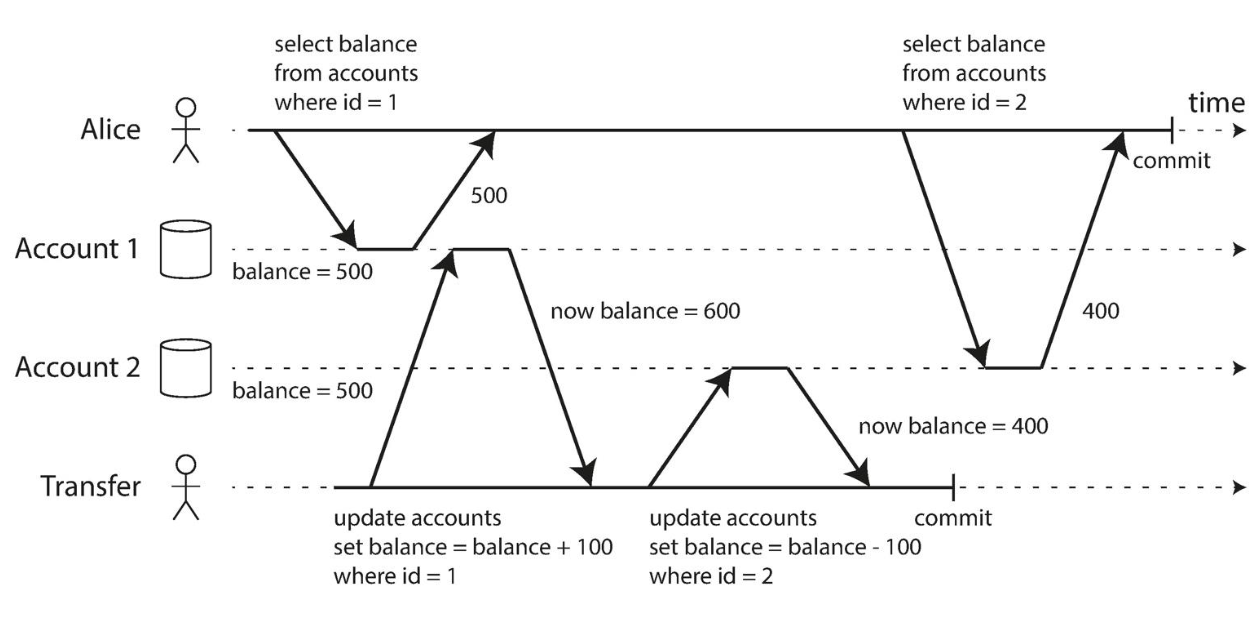
\includegraphics{images/12/readcommitted_issue.png}
   \caption{Read committed issue: Alice might think that her whole balance is 900, whilst it is 1000.}
   \label{fig:12/readcommitted_issue}
\end{figure}
% \begin{definition}
%    [Phantom Read]
%    A \textbf{phantom read} occurs when a transaction reads a set of records that satisfy a certain condition, but when it reads the same records again, the set of records has changed.

\subsection{Snapshot Isolation}
Snapshot isolation is a more relaxed isolation level than serializable isolation, but it is still stricter than Read Committed isolation.

In snapshot isolation, a transaction reads a snapshot of the database at the beginning of the transaction and writes to the database at the end of the transaction.

The snapshot allows transactions to see all the data that was commited at the start of the transaction.

% // TODO there is some other stuff about explicit locks, I'm not sure how important it is, the slides are a bit messed up

\note{It is possible to use at databases some techniques for locking the database, using locks or atomic operations. 
However it is costful}

\section{Write Skew and Phantoms}

\begin{paracol}{2}
   
   \begin{definition}
      [Write Skew]
      A \textbf{write skew} occurs when two transactions read the same data, then update ---possibly separate--- objects based on the read data, and then commit, causing a conflict.
   \end{definition}
   
   \switchcolumn

   \begin{figure}[htbp]
      \centering
      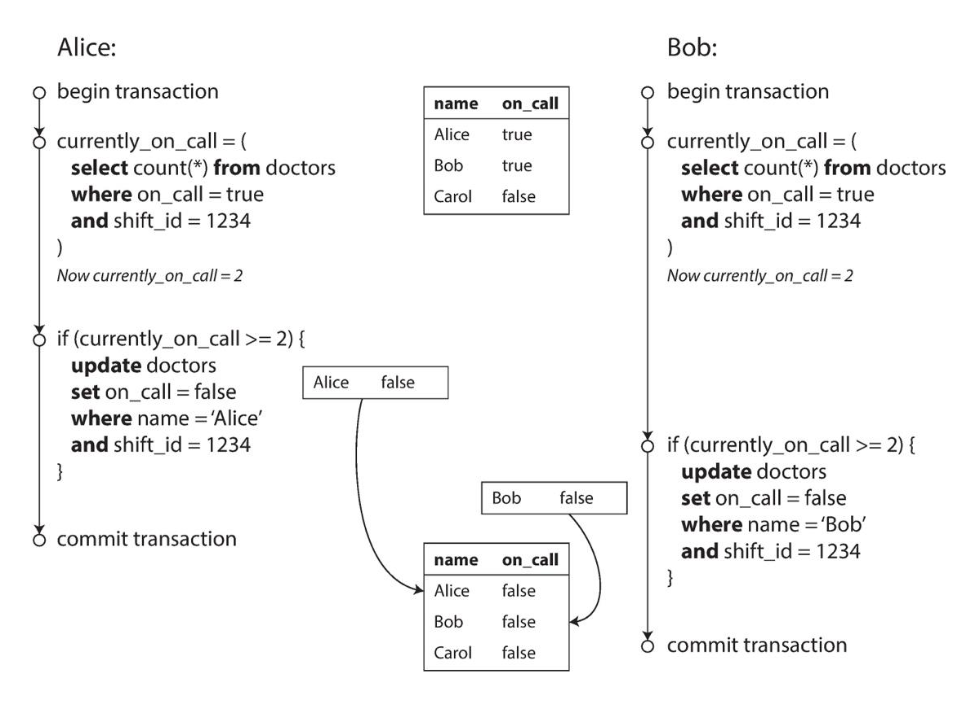
\includegraphics{images/12/write_skew.png}
      \caption{Both doctors read that \lstinline|currently_on_call >= 2| and ``leave the hospital'', causing no doctor to be on call \frownie.}
      \label{fig:12/write_skew}
   \end{figure}
\end{paracol}

There are some techniques to avoid write skew, such as using row locks or atomic operations, but we did not discuss them pretty much.



\chapter{Type Inference}
\begin{figure}[htbp]
   \centering
   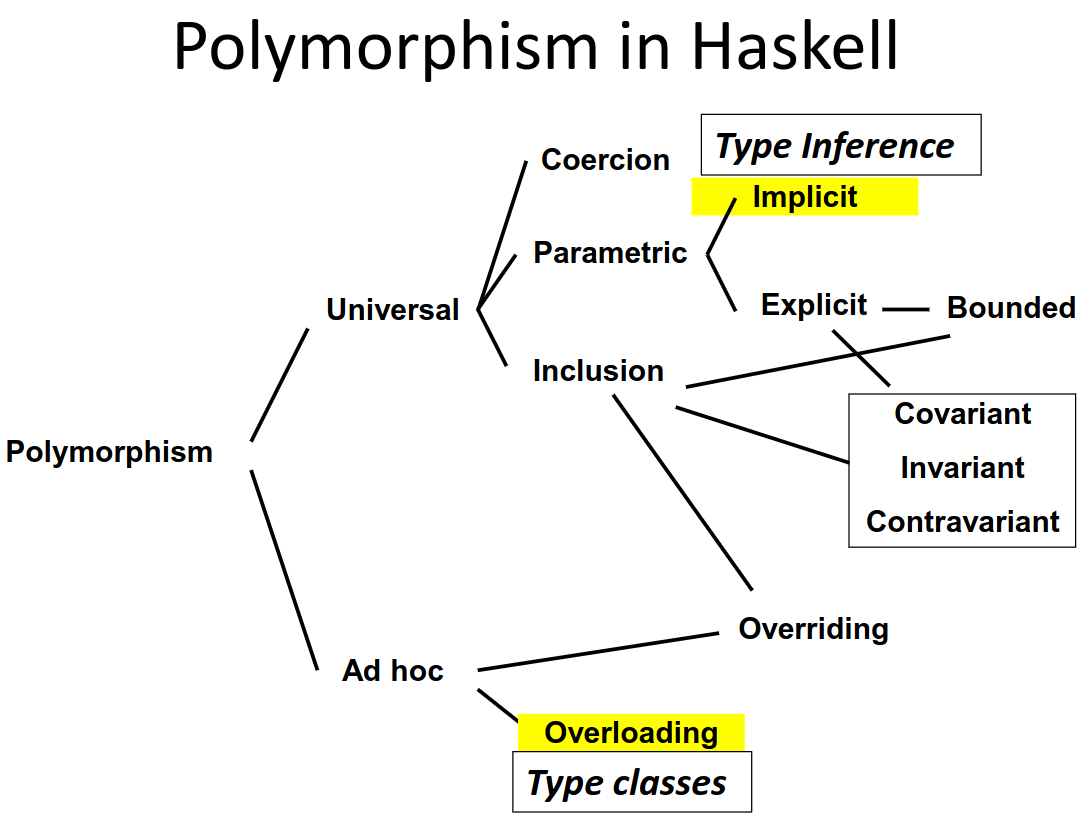
\includegraphics{images/haskell_polymorphism.png}
   \caption{Haskell Polymorphism Recap}
   \label{fig:haskell_polymorphism}
\end{figure}

\section{Overloading}
Haskell allows \textbf{overloading} even of \textbf{primitive types}:
the code to be executed is determined by the type of the arguments,
leading to have \textit{early binding} in \textit{statically} typed languages
or \textit{late binding} in \textit{dynamically} typed languages.

In Haskell we can write the following, but what is the type?
\begin{lstlisting}
   sqr x = x * x
\end{lstlisting}

When considering overloading besides arithmetic, we find that some functions are \textbf{fully polymorphic}:
\begin{lstlisting}
   length :: [w] -> Int
\end{lstlisting}

While others not so much;
for example, \textit{membership} works only for types that support equality,
while \textit{sorting} works only for types which support \textit{ordering}. 
\begin{lstlisting}
   member :: [w] -> w -> Bool
   sort :: [w] -> [w]
\end{lstlisting}

\section{Type Classes}
\textbf{Type Classes} solve many overloading problems concerning arithmetic and equality (and similar properties) support.

The idea is to generalize ML’s eqtypes to arbitrary types
and provide concise types to describe overloaded
functions, so no exponential blow-up (i.e. defining functions for every possible combination of type arguments).\\
Type classes allow users to define functions using overloaded
operations {---}e.g. square, squares, and member{---} and to
declare new collections of
overloaded functions: equality and arithmetic
operators are not privileged built-ins.
Haskell's solutions fits perfectly within type inference framework.

The intuition is that a sorting function may allow to be passed a comparison \lstinline|cmp| operator as argument,
thus making the function parametric.
\begin{lstlisting}
   qsort:: (a -> a -> Bool) -> [a] -> [a]
   qsort cmp [] = []
   qsort cmp (x:xs) = qsort cmp (filter (cmp x) xs) ++ [x] ++
   qsort cmp (filter (not.cmp x) xs)
\end{lstlisting}

Developing this idea, consider rewriting the parabola function to take operators as argument
\begin{lstlisting}
   parabola x = (x * x) + x
   parabola' (plus, times) x = plus (times x x) x
\end{lstlisting}
Here the extra parameter is a \textit{\textbf{dictionary}} that provides implementations for the overloaded ops.
These implies rewriting calls to pass appropriate implementations for plus and times:
\begin{lstlisting}
   y = parabola'(intPlus,intTimes) 10
   z = parabola'(floatPlus, floatTimes) 3.14
\end{lstlisting}

\begin{enumerate}
   \item Type class declarations
   \begin{enumerate}
      \item Define a set of operations, give it a name
      \item Example: \lstinline|Eq a| type class
      • operations \lstinline|==| and \lstinline|\=| with \lstinline|type a -> a -> Bool|
   \end{enumerate}
   \item Type class instance declarations
   \begin{enumerate}
      \item Specify the implementations for a particular type
      \item For \lstinline|Int| instance, \lstinline|==| is defined to be integer equality
   \end{enumerate}
   \item Qualified types (or Type Constraints)
   Concisely express the operations required on otherwise polymorphic type
   \lstinline|member:: Eq w => w -> [w] -> Bool|
\end{enumerate}

\labelitemize{
   \textit{implementation summary}
}{
   \begin{enumerate}
      \item Each overloaded symbol has to be introduced in at least one type class
      \item The compiler translates each function that uses an overloaded symbol into a function with an extra parameter: the dictionary.
      \item References to overloaded symbols are rewritten by the compiler to lookup the symbol in the dictionary.
      \item The compiler converts each type class declaration into a dictionary type declaration and a set of selector functions.
      \item The compiler converts each instance declaration into a dictionary of the appropriate type.
      \item The compiler rewrites calls to overloaded functions to pass a dictionary. It uses the static, qualified type of the function to select the dictionary.
   \end{enumerate}
}

\subsection{Compositionality}
\begin{lstlisting}
   class Eq a where
   (==) :: a -> a -> Bool
   instance Eq Int where
   (==) = intEq -- intEq primitive equality
   instance (Eq a, Eq b) => Eq(a,b) where
   (u,v) == (x,y) = (u == x) && (v == y)
   instance Eq a => Eq [a] where
   (==) [] [] = True
   (==) (x:xs) (y:ys) = x==y && xs == ys
   (==) _ _ = False
\end{lstlisting}

\subsection{Compound Translation}
\newpage
\subsection{Subclasses}
\begin{paracol}{2}
   \vspace{\fill}
   
   A subclass declaration expresses this relationship:
   \begin{lstlisting}
      class Eq a => Num a where
      (+) :: a -> a -> a
      (*) :: a -> a -> a
   \end{lstlisting}
• With that declaration, we can simplify the type of the function

\begin{lstlisting}
   memsq :: (Eq a, Num a) => a -> [a] -> Bool
   memsq x xs = member (square x) xs
\end{lstlisting}

\vspace{\fill}
\switchcolumn

\begin{figure}[htbp]
   \centering
   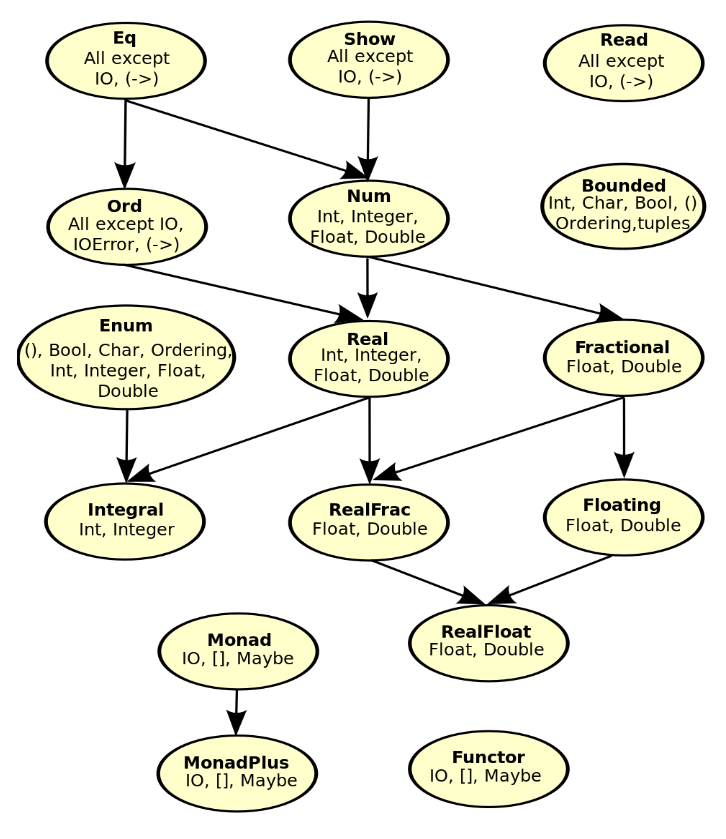
\includegraphics{images/haskell_subclasses.png}
   \caption{Haskell Subclasses relationships}
   \label{fig:haskell_subclasses}
\end{figure}

\end{paracol}

\subsection{Deriving}
For Read, Show, Bounded, Enum, Eq, and Ord, the compiler
can generate instance declarations automatically.
\begin{lstlisting}
   data Color = Red | Green | Blue
      deriving (Show, Read, Eq, Ord)
   
   Main>:t show
   show :: Show a => a -> String
   Main> show Red
   "Red"
   Main> Red < Green
   True
   Main>:t read
   read :: Read a => String -> a
   Main> let c :: Color = read "Red"
   Main> c
   Red
\end{lstlisting}

\subsection{Numeric Literals}
\begin{lstlisting}
   class Num a where
      (+) :: a -> a -> a
      (-) :: a -> a -> a
      fromInteger :: Integer -> a
      -- Even literals are overloaded.
      -- 1 :: (Num a) => a
      ...

   inc :: Num a => a -> a
   inc x = x + 1
\end{lstlisting}

\labelitemize{
   \textit{Advantages}
}{
   \setlength{\leftskip}{1em}
   Numeric literals can be interpreted as values of any
   appropriate numeric type,
   for example: 1 can be an Integer or a Float or a user-
   defined numeric type.
}

\subsection{Missing Notes}
Look at slides $34...64$ for more on Type Inference.

\section{Inferencing types}
In standard type checking the compiler examine body of each function and uses declared types to check agreement;
type inference instead consists in examining code without type information, and infer the
most general types that could have been declared

\subsection{Steps schematics}
\begin{figure}[htbp]
   \centering
   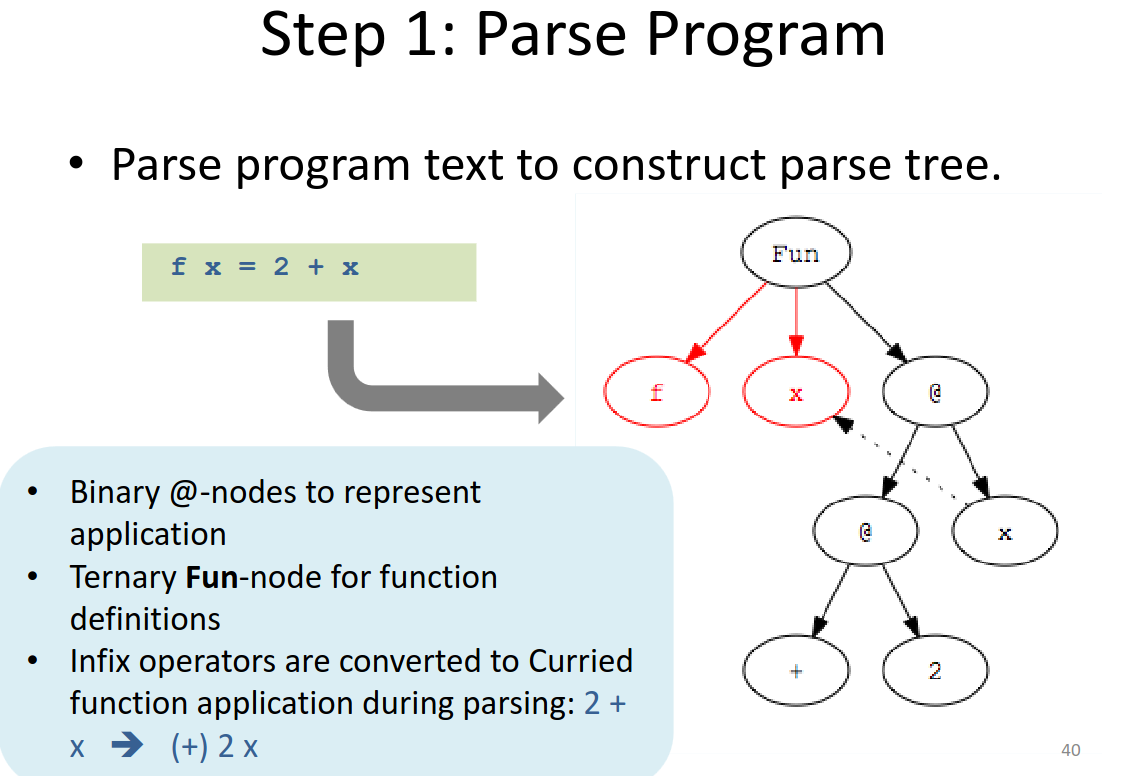
\includegraphics[width=0.4\columnwidth]{images/typeinference_step1.png}
   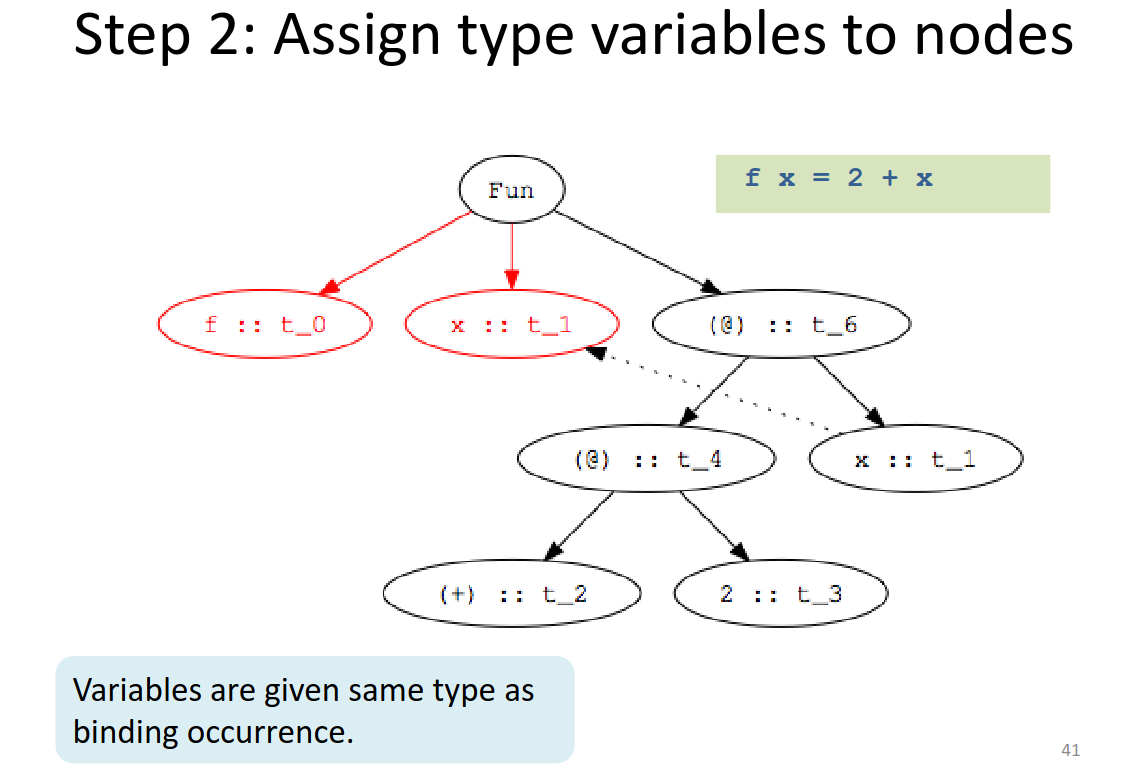
\includegraphics[width=0.4\columnwidth]{images/typeinference_step2.png}
   \label{fig:typeinference_step1_2}
\end{figure}

% \begin{figure}[htbp]
%    \centering
%    \label{fig:typeinference_step2}
% \end{figure}

\textbf{Constraints} can be deduced from (function) \textit{Application} nodes \lstinline|f x| and from \textit{Abstractions} \lstinline|f x = e|.

\begin{figure}[htbp]
   \centering
   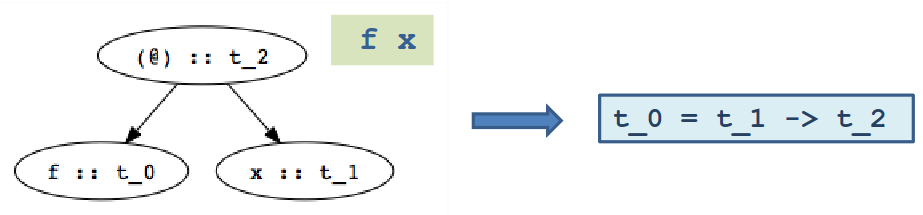
\includegraphics{images/typeinference_constraints_application.png}
   \caption{Deducing constraints from function application}
   \label{fig:typeinference_constraints_application}
\end{figure}
\begin{itemize}
   \item Type of \lstinline|f| (\lstinline|t_0| in figure) must be $domain \longrightarrow range$.
   \item \textbf{Domain} of \lstinline|f| must be type of argument \lstinline|x| (\lstinline|t_1|)
   \item \textbf{Range} of f must be result of application (\lstinline|t_2|)
   \item \textbf{Constraint}: \lstinline|t_0 = t_1 -> t_2|
\end{itemize}

\begin{figure}[htbp]
   \centering
   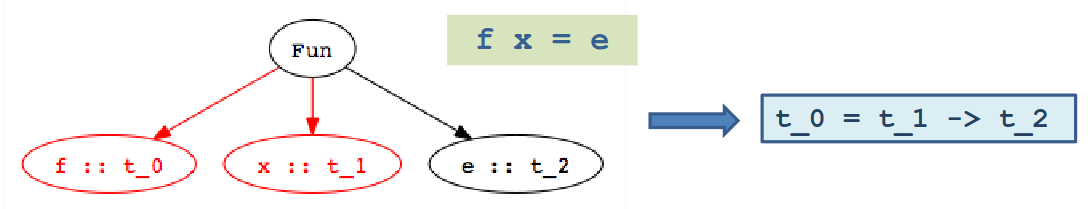
\includegraphics{images/typeinference_constraints_abstraction.png}
   \caption{Deducing constraints from abstractions}
   \label{fig:typeinference_constraints_abstraction}
\end{figure}

\begin{itemize}
   \item Type of \lstinline|f| (\lstinline|t_0|) must $domain \longrightarrow range$
   \item \textbf{Domain} is type of abstracted variable \lstinline|x| (\lstinline|t_1|)
   \item \textbf{Range} is type of function body \lstinline|e| (\lstinline|t_2|)
   \item \textbf{Constraint}: \lstinline|t_0 = t_1 -> t_2|
\end{itemize}

\begin{figure}[htbp]
   \centering
   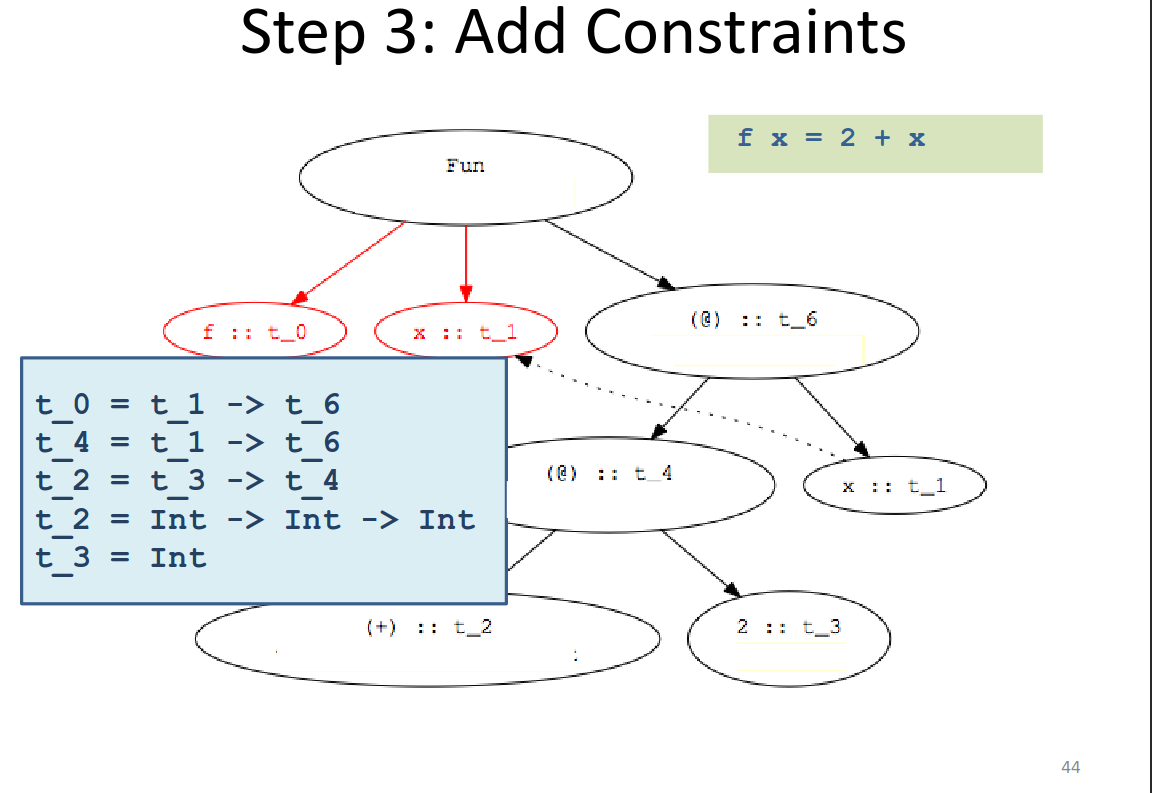
\includegraphics[width=0.4\columnwidth]{images/typeinference_step3.png}
   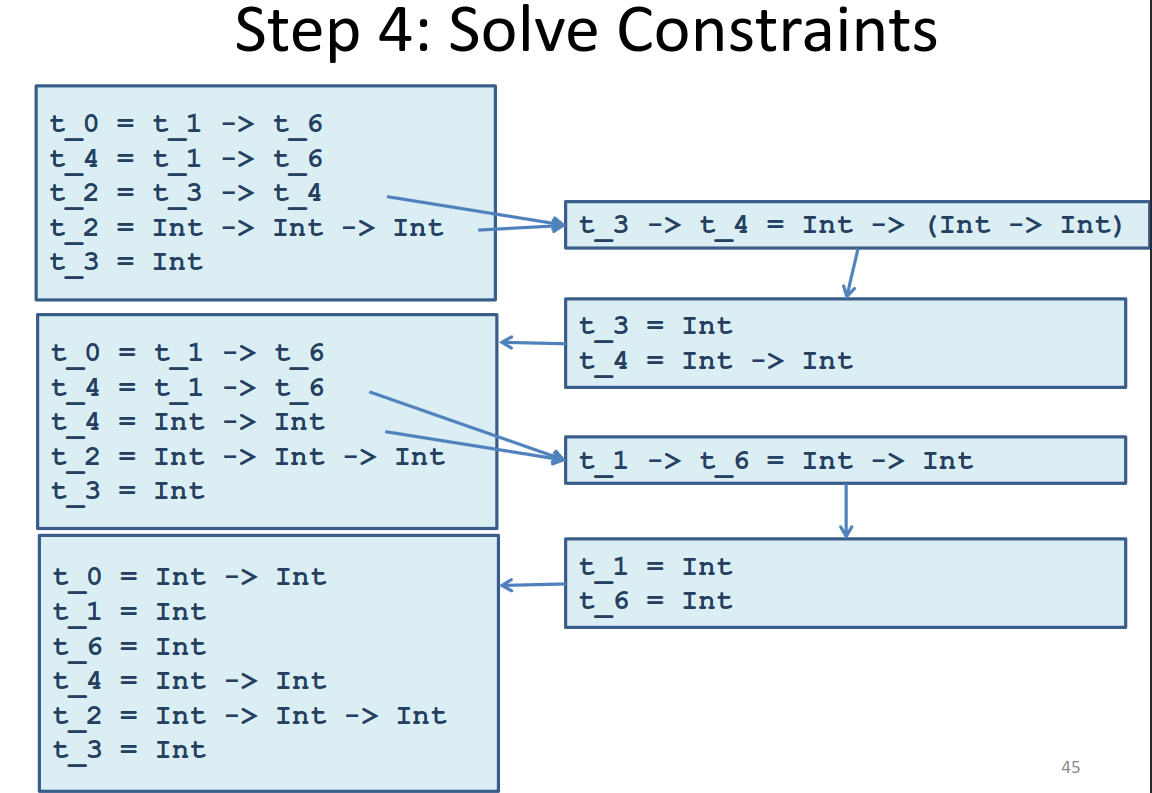
\includegraphics[width=0.4\columnwidth]{images/typeinference_step4.png}
   \label{fig:typeinference_step3_4}
\end{figure}

\begin{figure}[htbp]
   \centering
   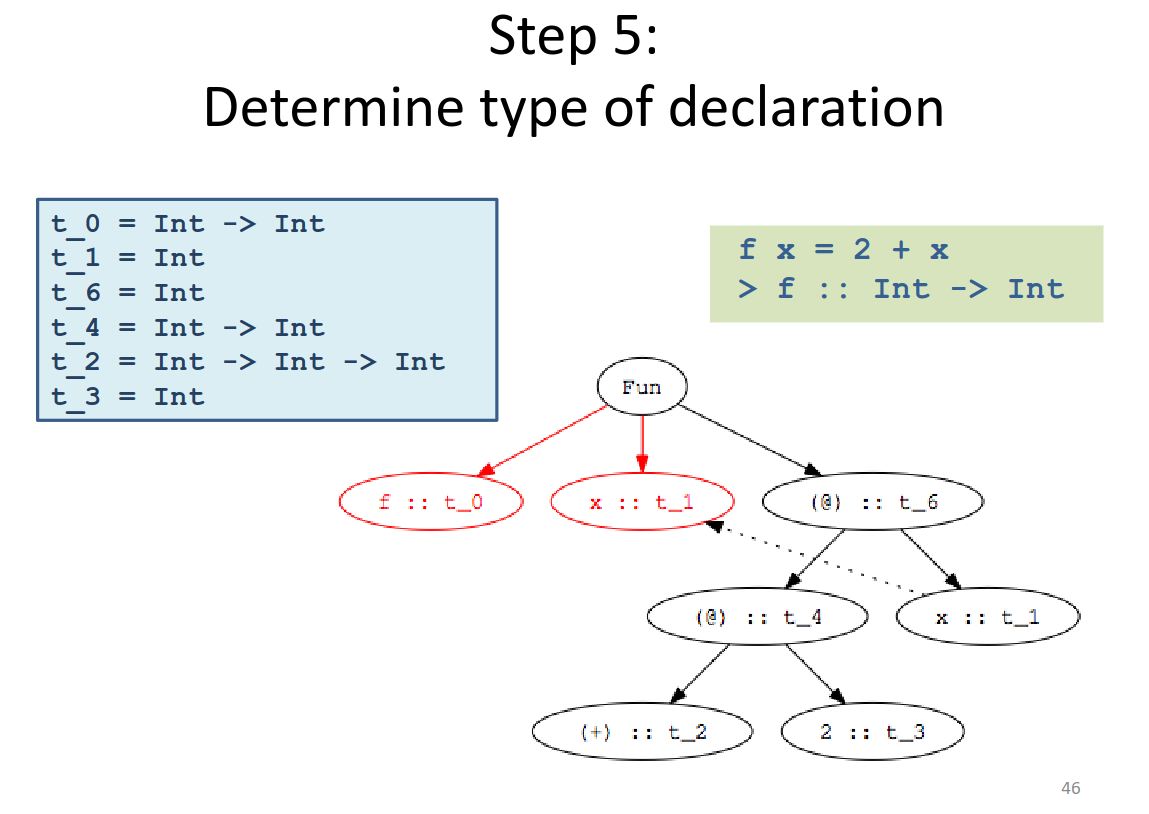
\includegraphics[width=0.4\columnwidth]{images/typeinference_step5.png}
   \label{fig:typeinference_step5}
\end{figure}

\subsubsection{Steps summary}
\begin{enumerate}
   \item Parse program to build parse tree
   \item Assign type variables to nodes in tree
   \item Generate constraints:
   \begin{enumerate}
      \item From environment: constants (\lstinline|2|), built-in
      operators (\lstinline|+|), known functions (\lstinline|tail|).
      \item From shape of parse tree: e.g., application and
      abstraction nodes.
   \end{enumerate}
   \item Solve constraints using unification
   \item Determine types of top-level declarations
\end{enumerate}

\subsection{Polymorphism}

In general \textbf{unconstrained} type variables become \textbf{polymorphic types};
for instance, in the example below \lstinline|t_4| is unconstrained, hence we get a polymorphic type:
\begin{lstlisting}
   f g = g 2
   > f :: (Int -> t_4) -> t_4
\end{lstlisting}
\nl

For functions with multiple clauses, i.e. \textit{polymorphic datatypes},
for each clause a separate type is inferred, 
and then the resulting types are combined by adding constraints such as that all clauses have the same type.
In case of \textit{recursive calls}:
the function has same type as its definition.

\begin{lstlisting}
   append ([],r) = r
   append (x:xs, r) = x : append (xs, r)
\end{lstlisting}

\begin{enumerate}
   \item Infer type of each clause
   \begin{enumerate}
      \item First clause:
      \begin{lstlisting}
   > append :: ([t_1], t_2) -> t_2
      \end{lstlisting}
      \item Second clause:
      \begin{lstlisting}
   > append :: ([t_3], t_4) -> [t_3]
      \end{lstlisting}
   \end{enumerate}
   \item Combine by equating types of two clauses
   \begin{lstlisting}
   > append :: ([t_1], [t_1]) -> [t_1]
   \end{lstlisting}
\end{enumerate}

\subsection{Overloading}
In presence of \textbf{overloading} (\textit{Type Classes}), type inference infers a \textbf{qualified type} \lstinline|Q => T|
\begin{itemize}
   \item T is a Hindley Milner type, inferred as seen before
   \item Q is set of type class predicates, called a constraint
\end{itemize}
\begin{lstlisting}
   example :: Ord a => a -> [a] -> Bool
   example z xs = 
      case xs of
         [] -> False
         (y:ys) -> y > z || (y==z && ys == [z])
\end{lstlisting}

\begin{paracol}{2}
   \colfill
   In the example \textbf{Type} \lstinline|T| is \lstinline|a -> [a] -> Bool|
   while the \textbf{Constraint} \lstinline|Q| is \lstinline|{ Ord a, Eq a, Eq [a]}|.
   \lstinline|Q| later simplifies\footnote{According to some rules not discussed here} to \lstinline|Ord a|
   \colfill
   \switchcolumn

   \begin{itemize}
      \item \lstinline|Ord  a| because \lstinline|y>z|
      \item \lstinline|Eq a| because \lstinline|y==z|
      \item \lstinline|Eq [a]| because \lstinline|ys == [z]|
   \end{itemize}
\end{paracol}
\subsubsection{Functor and \texttt{fmap}}
\chapter{Bluetooth}

Bluetooth is a wireless technology standard for exchanging data over short distances (using short-wavelength UHF radio waves in the ISM band from 2.4 to 2.485 GHz) from fixed and mobile devices, and building personal area networks (PANs). It was originally conceived as a wireless alternative to RS-232 data cables. Bluetooth is managed by the Bluetooth Special Interest Group (SIG), which has more than 35,000 member companies in the areas of telecommunication, computing, networking, and consumer electronics. The IEEE standardized Bluetooth as IEEE 802.15.1, but no longer maintains the standard. The Bluetooth SIG oversees development of the specification, manages the qualification program, and protects the trademarks. A manufacturer must meet Bluetooth SIG standards to market it as a Bluetooth device. A network of patents apply to the technology, which are licensed to individual qualifying devices.

\section{Architecture}
\begin{figure}[htbp]
   \centering
   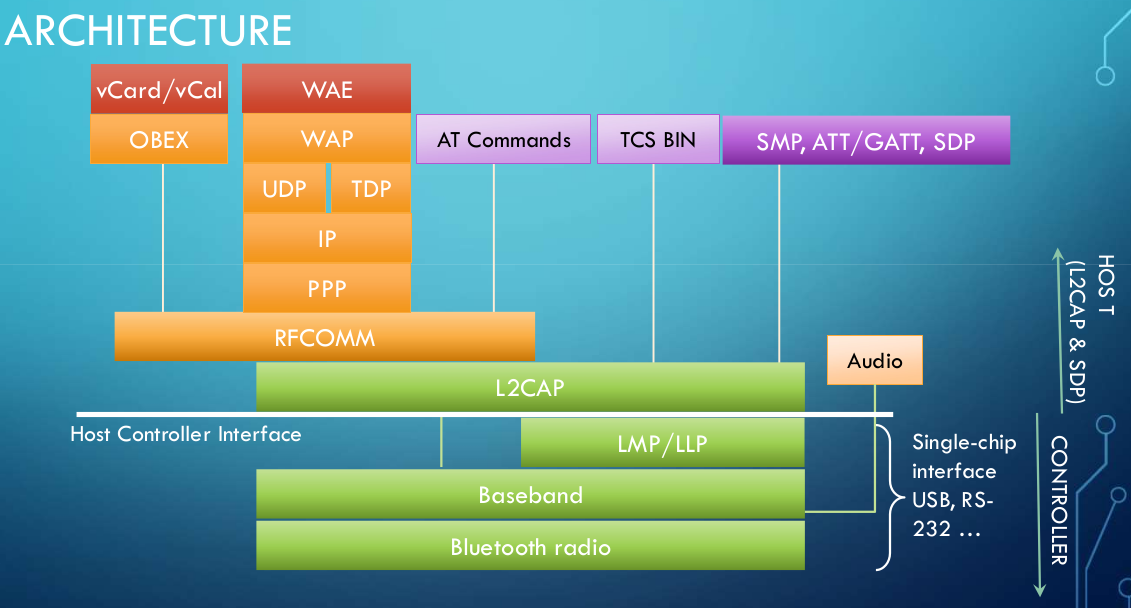
\includegraphics{images/bluetooth_architecture.png}
   \caption{Architecture of Bluetooth.}
   \label{fig:bluetooth_architecture}
\end{figure}

The bluetooth core system is composed of one or more \textbf{controllers} and a \textbf{host}. The controller is a microcontroller that executes the physical layer and the link layer, while the host is a microcontroller that executes the higher layers of the protocol stack. The host communicates with the controller through a serial interface.\\
The host comprises all layer below the HCI (Host Controller Interface) shown in Fig. \ref{fig:bluetooth_architecture} , while the controller comprises the HCI and the layers below.

\note{TODO check this}

The core protocols are various:
\begin{itemize}
   \item \textit{Radio}: defines the specification of the radio frequencies.
   \item \textit{Baseband}: defines the low level procedures of the PHY layer
   \item \textit{LMP} (link management protocol - for \texttt{BR/EDR}) / \textit{LLP} (link layer protocol - for \texttt{BLE}): setup and control of the link.
   \item \textit{HCI} (Host Controller Interface): interface between hardware and software.
   \item \textit{L2CAP} (Logical Link Control and Adaptation): higher-level protocol multiplexing,
   packet segmentation and reassembly, and the conveying of quality of service information.
   \begin{itemize}
      \item Provides an interface to higher level protocols and applications to transmit and receive data packets, up
      to 64 kilobytes in length.
      \item Implements flow control and retransmission modes.
   \end{itemize}
   \item \textit{SDP}: Service Discovery Protocol
\end{itemize}

\subsection{\texttt{BR/EDR} vs \texttt{BLE}}
BR/EDR (Basic Rate/Enhanced Data Rate), used for streaming audio and other data. It is a point-to-point connection, and can connect up to 7 devices.\\
It is connection-oriented, meaning that the a link between two devices is kept even if no data is flowing;
There are however \textit{sniff modes} which allow devices to sleep and thus to save energy.\\
Peak transmit current is about $25mA$, which is low compared to other wireless technologies, but still not enough low for very low-power devices or coin cell batteries.
\nl

BLE (Bluetooth Low Energy) is a different protocol, designed for ultra low power consumption. It is connectionless, and can connect up to 40 devices.\\
It exploits short packets to reduce TX peak current and RX time, and less channels to improve discovery and connection time, ultimately resulting in overall lower power consumption, with $20mA$ as peak transmit current, and $6\mu A$ as average current.

BLE operates at 2.4GHz and uses 40 channels with FDMA (Frequency Division Multiple Access), with 2MHz spacing. IChannels 37,38,39 are used for connection, discovery and broadcast, while the others for data.
The maximum data rate is $1Mbps$, however this protocol is meant for smaller packets, it is not optimized for file transferring.\\
Each channel is divided into time units (events), either
\begin{itemize}
   \item \textit{Advertising} events
   \item \textit{Connection} events
\end{itemize}


\section{Network topologies}
\begin{paracol}{2}
   
   Two topologies are possible, \textit{Piconet} and \textit{Scatternet}.
   The Scatternet is a network of Piconets, where a device can be part of multiple Piconets, and thus can act as a bridge between them.

   The master is unique in each piconet and synchronizes it, besides it also controls the access to the channel of all slave stations.\\
   In BE/EDR up to 7 slaves can be connected to a master, while in BLE there is no limit, but a device may be in only one piconet.
   \switchcolumn
   \begin{figure}[htbp]
      \centering
      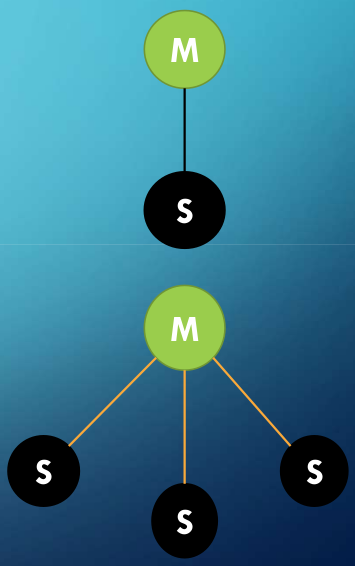
\includegraphics[width=0.45\columnwidth]{images/bluetooth_topology.png}
      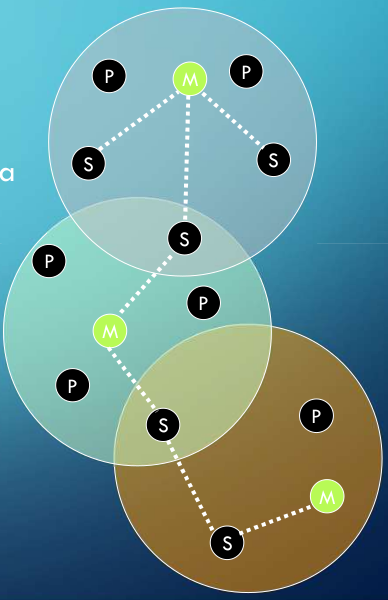
\includegraphics[width=0.45\columnwidth]{images/bluetooth_scatternet.png}
      \caption{Devices sharing the same channel form a \textit{Piconet}, with one Master and ---possibly--- multiple slaves.\\
      Multiple Piconets can be connected to form a \textit{Scatternet}.}
      \label{fig:bluetooth_topology}
   \end{figure}
\end{paracol}

\newpage
\section{Baseband layer}
\section{Phyisical Layer}
\begin{figure}[htbp]
   \centering
   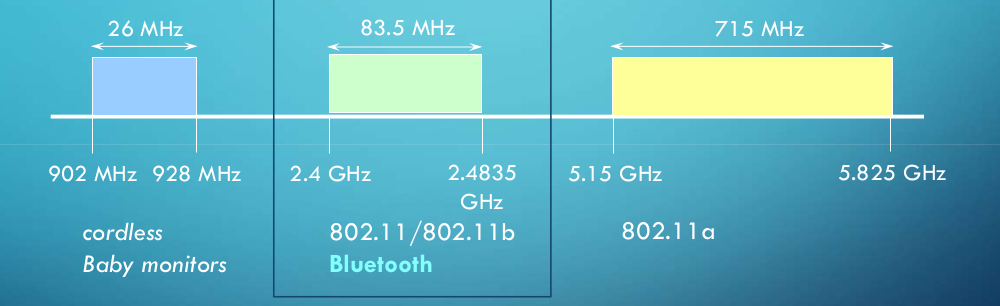
\includegraphics{images/bluetooth_frequencies.png}
   \caption{Operating bluetooth frequencies}
   \label{fig:bluetooth_frequencies}
\end{figure}

\section{Substates}
The BLE protocol defines many substates, which are used to manage the power consumption of the device. The device can switch between these states depending on the activity it is performing.

\labelitemize{Conn Establishment}{
   \begin{itemize}
      \item Page
      \item Page scan
      \item Page response
      \item Inquiry
      \item Inquiry scan
      \item Inquiry response
   \end{itemize}
}

\labelitemize{Conn state}{
   \begin{itemize}
      \item Active mode
      \item Sniff mode
      \item Hold mode
      \item Park
   \end{itemize}
}

\part{Federica Paganelli}
% \minitoc
\parttoc
% \parttoc
\chapter{Introduction}
\section*{27 - Settembre}
\section{Product based}
In \textit{Project-based SE} there is loop which nowdays cripples software since its early stages of development.
This is due to mutable nature of requirements, which often change throughout time along the features implemented by the software.
\begin{center}
\begin{tikzpicture}
    \node[draw=white,align=left] (A) at (1.5,3) {Problem};
    \node[draw=white,align=left] (B) at (0,0) {Requirements};
    \node[draw=white,align=left] (C) at (3,0) {Software};

    \path [->] (A) edge node[left] {} (B);
    \path [->] (B) edge node[left] {} (C);    
    \path [->] (C) edge node[left] {} (A);    
\end{tikzpicture}
\end{center}

\textit{Product-based SE} is opposed to \textit{Project-based SE} and the above pictures changes as follows.

\begin{center}
\begin{tikzpicture}
    \node[draw=white,align=left] (A) at (1.5,3) {Opportunity};
    \node[draw=white,align=left] (B) at (0,0) {Features};
    \node[draw=white,align=left] (C) at (3,0) {Software};

    \path [->] (A) edge node[left] {} (B);
    \path [->] (B) edge node[left] {} (C);    
    \path [->] (C) edge node[left] {} (A);    
\end{tikzpicture}
\end{center}

\section{Agile}
Agile is a collection of principles and methods applied in the software development field.
\nl

Opposed to project-based SE, in Agile the client is requested to express the requirements not in technical terms but in features.

Agile suggests an incremental development model

\subsection*{Principles}
\begin{enumerate}
    \label{subsec:agile_principles}
    \item Satisfy customer through early and continuous delivery of valuable software
    \item Welcome changing requirement, even late in development.
    Agile processes harness change for the customer's comptetitive advantage
    \item Deliver working software frequently, from a couple of weeks to a couple of months, with a preference to the shorter timescale
    \item Business people and devs must work together daily throughout the prokect
    \item Build porjects around motivated individuals and give them the environment and support they need
    \item The most efficient and effective method of conveying information to and within a dev team is face-to-face conversation
    \item Working software is the primary measure of progress
    \item Agile processes promote sustainable dev 
    \item Continuous attention to technical excellence and good design enhances agility
    \item Simplicity i.e. art of maximizing the amount of work not done is essential
    \item The best architectures, requirements, and designs emerge from self-organizing teams.
\end{enumerate}

Extreme Programming was proposed as part of the agile methodology

\section{Scrum}
Since requirements changes are rather frequent, long-term plans are unreliable,
hence SE aims to formulate short-term plans.

Scrum is found on \textbf{empiricism} and \textbf{lean thinking}; it asserts that knowledge comes from experience, and that decisions should be made on observations.

Other key terms are code \textbf{Transparency} among the team and with the customer, \textbf{Inspection} of produced code and software (artifacts), \textbf{Adaptation} to changes in features and requirements.

The \textbf{Scrum Team} is composed by:
\begin{enumerate}
    \item \textbf{Product Owner}: must ensure that the dev team is always focused on the goal
    \item \textbf{Scrum Master}: Scrum expert which drives the team to apply properly the Scrum framework.
    \item \textbf{Developers}: actual monkeys people which write code
\end{enumerate}

In scrum SW is developed in \textbf{sprints}, i.e. fixed-length periods with a specific goal to be achieved.

\begin{itemize}
    \item Product backlog: to-do list of items to be implemented
    \item Timeboxed sprints
    \item Self-organizing teams
\end{itemize}

...
\textbf{Prod Backlog Revised}\\
\textbf{PBI Estimation Metrics}

\subsection{Timeboxed Sprints}
Even if at the end of a srpint the goal hasn't been reached, "no worries", the work stops anyway;
there will be a new sprint which will include the work which has not been implemented in the previous one.

\subsection{Scrum Meetings}

\subsection{Agile activities}
Test automation
Continuous integration

\subsection{Sprint reviews}
At the end of each sprint there is a review meeting which involves the \textit{whole} team.
The \textit{product owner} has the ultimate authority to decide wether the sprint goal has been reached or not.
The sprint review should include a process review, in which the whole team shares ideas on how to improve their way of working.

\textbf{Team size}\nl

\section{5 - Ottobre}



\chapter{IEEE 802.11}

\begin{figure}[htbp]
   \centering
   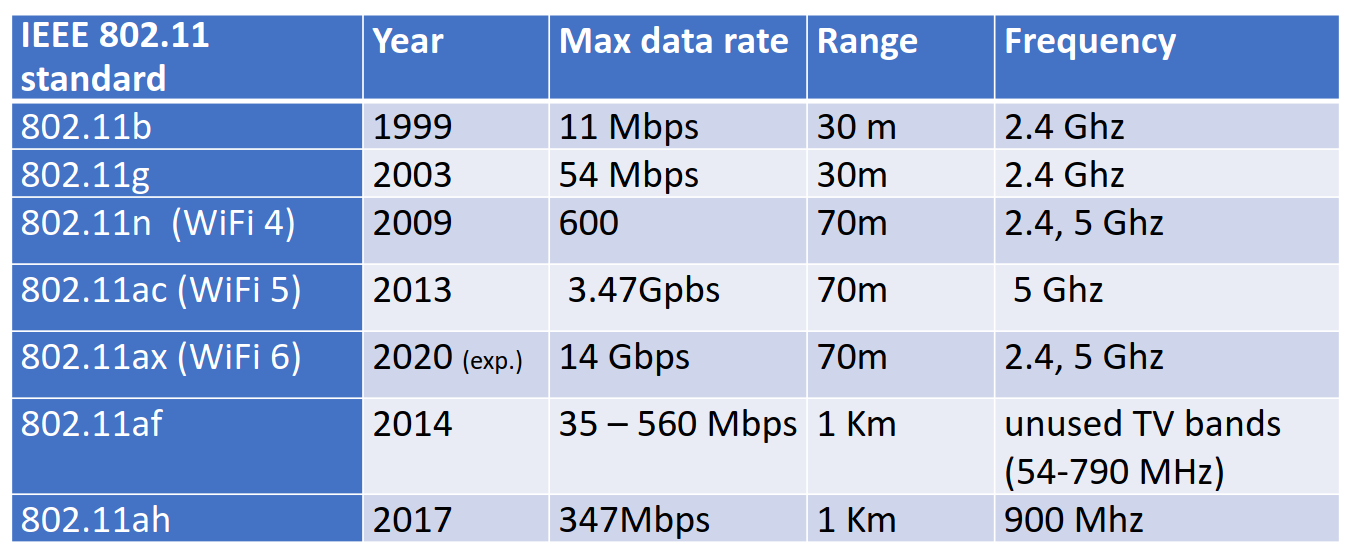
\includegraphics{images/ieee_bgn.png}
   \caption{IEEE 802.11 standards}
   \label{fig:ieee_bgn}
   All these standards \texttt{use \texttt{CSMA/CA} for multiple access}, and have base-station and ad-hoc network versions
\end{figure}

IEEE 802.11 standards refer to the \textit{Physical} Layer.
In case of an AP (Access Point), every station must channel its communication through the AP to talk to any other. Otherwise, in an \textit{Ad-Hoc} network, stations can communicate directly with each other.

TODO

\note{TODO non ci sono domande su questa cose nel pdf}
\chapter{Fabric}
``Fabric'' is the term used to refer to the \textit{interconnection} between nodes of a datacenter.\\
\ul{Cabling is of paramount importance.}
\note{Prof. Cisternino learnt it ``the hard way'' when he performed the cabling of the first UniPi datacenter by himself}
\begin{enumerate}
   \item Maintenance
   \item Cooling
   \begin{enumerate}
      \item Cables may heat up
      \item Cables may obstruct air flow
   \end{enumerate}
   \item Determines which machines interact with each other (\textit{fabric})
   \item Bandwidth
   \item Not neglectable cost
\end{enumerate}

We refer to North-South traffic indicating the traffic outgoing and incoming to the datacenter (internet), while we refer to East-West as the internal traffic between servers.
Most of the network (or fabric) traffic is processed horizontally (North-South traffic)\footnote{Seems odd that ``horizontal'' refers to North-South traffic, but that's how it is.}.


\section{Bandwidth and Storage implications}
\label{sec:bandwidth_storage}
A standard datacenter has servers connected with 25Gbit links in both directions, summing up to 50Gbit total bandwidth.
Current SSDs using NVMe provide much more, about $3.5 GB/s$, making \ul{4 drives are enough to saturate a 100Gbit/s link.}\\
We moved from a situation where the \textbf{bottleneck} were slow Hard Drives, to the current one where the bottleneck is the ---network--- \textbf{bandwidth}.\\
Recently the PCI 3.0, which lasted very long ---providing roughly$\sim\texttt{120Gbit/s}$ using 16 pin---, suddenly become unsufficient to handle the needed traffic.

Considering this, \ul{datacenters must be designed to allow \textit{Terabytes} of data to be moved in east-west traffic.}

\begin{center}
   \ul{\textit{The \textbf{fabric} is the glue that makes the datacenter possible.}}
\end{center}

Besides, a single server is \textit{unable} to handle 10TBs of data and handling requests from 3000 users simultaneously. It is necessary to \textbf{distribute} the requests.

HDDs are still currently used for \textbf{cold storage};
CPUs will access data exclusively from SSDs, and sometimes the server is shipped with on board \textbf{full-flash storage}.\\
The difference in price between SSDs and HDDs becomes negligible since you pay for top CPU, top GPU, top RAM;
furthermore, you can't waste ---the high amount of--- energy ---consumed by such components--- by waiting for a slow drive.

SSDs have a known write limit, but today, the usually last enough time: if you write the whole disk every day it will last for 5 years. Most-likely after five years you'd have to renew some components anyway, besides the failure is a predictable event.

\section{Cables and standards}
\subsection{Optical}
Electric current propagates at a speed $s = {\sim}0.6c$.
Hence \textbf{optical fiber} is ---at least in theory?--- faster.

\textbf{Lasers} are a coherent beam of equal fotons. It is possible to transfer energy through such fotons. Something resembling a laser is used for optical fibers.

Blu-Ray came out when scientists managed to create light using frequencies in the Blu area, which are the higher ones.
Currently, the best and most expensive optical fibers exploit blu-lasers as source of light.

Note that with optical you always need 2 fibers, one sending and the other receiving. The two possible connectors are \texttt{SC} and \texttt{LC}.
Sometimes the two ends of the cable are detachable so that the cables may be switched; this is useful because sometimes you may want to attach the TX cable on the RX plug and viceversa. 

\begin{figure}[htbp]
   \centering
   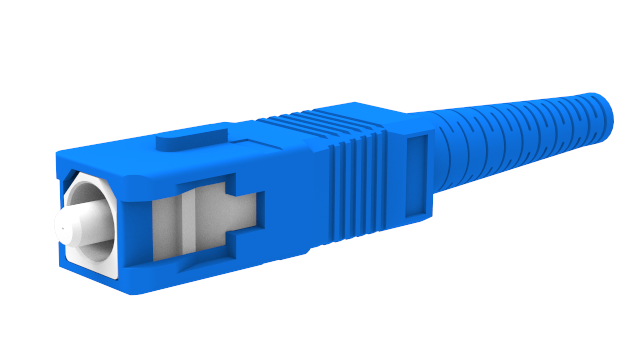
\includegraphics[width=0.25\columnwidth]{images/SC.png}
   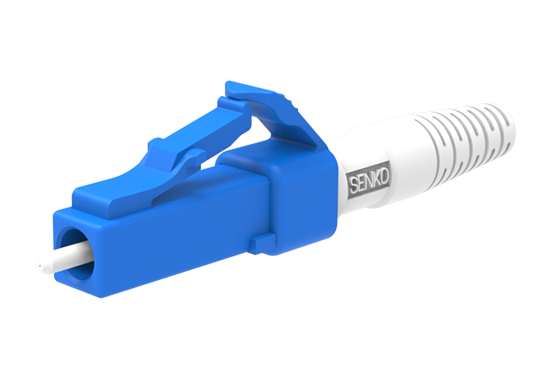
\includegraphics[width=0.25\columnwidth]{images/LC.png}
   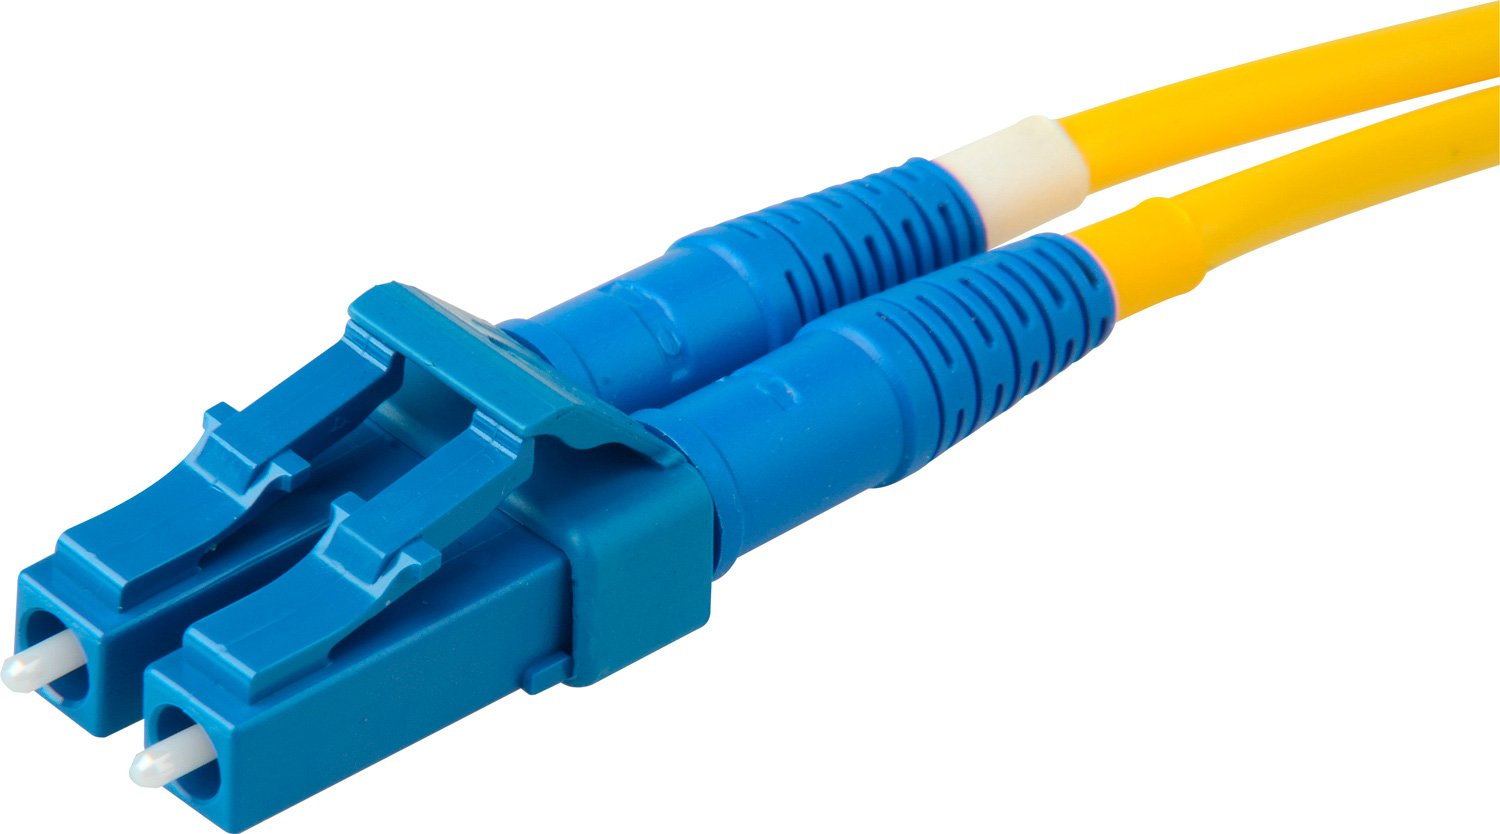
\includegraphics[width=0.25\columnwidth]{images/LC_coupled.JPG}
   \caption{\texttt{SC} and \texttt{LC} connectors}
   \label{fig:sc_lc_connectors}
\end{figure}

\subsection{Copper wires}
In case of electricity there are many aspects to be considered. Interferences, cable diameter/size, length, and also the fact that if a \texttt{1} has been transmitted for some time, it takes longer to transmit a \texttt{0}, due to the \textit{commutation} that must happen.
\nl

\begin{paracol}{2}
   \colfill
   \textbf{RJ45} is a standard physical interfaced for copper wires, which allows up to 1Gbit regularly.
   The \texttt{Cat 7} cables still use the RJ45 as connector and provide instead 10Gbit/s, but are very uncomfortable, they are so thick that they are difficult to bend.
   
   It is estimated that there have been installed $70 \times 10^9m$ of Ethernet cables, making them the most used.
   \colfill
   \switchcolumn

   \begin{figure}[htbp]
      \centering
      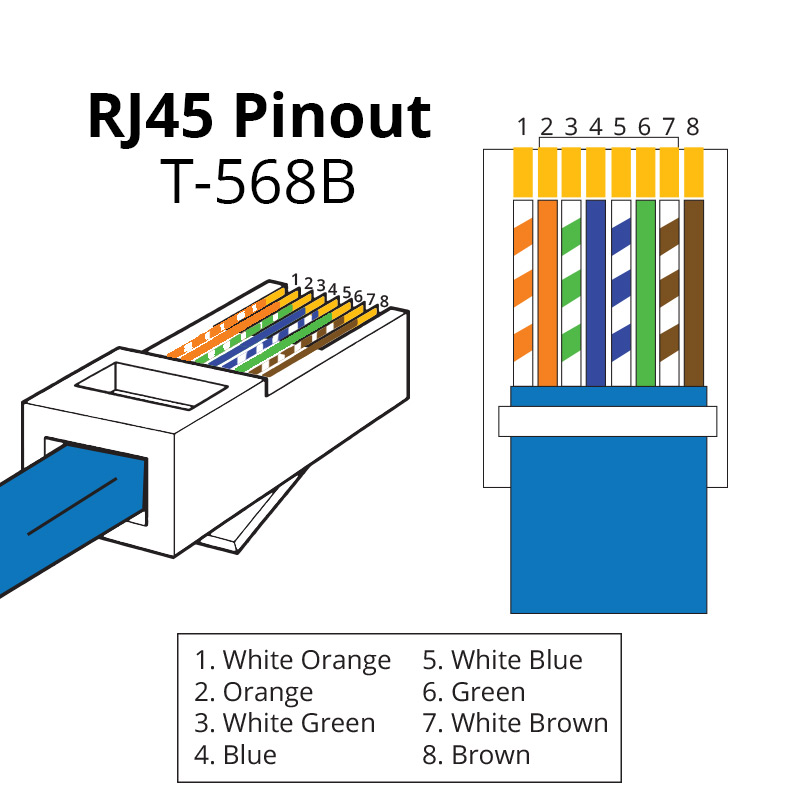
\includegraphics{images/RJ45_T568B.jpg}
      \caption{RJ45 - T568B}
      \label{fig:RJ45_T568B}
   \end{figure}
\end{paracol}

\subsection{SFP - Small Form-factor Pluggable}
There can be a cable with a LC in one side and a SC on the other side.
Instead of making switches with the optical plugs, switches were created with electrical plugs that would be able to host a \textbf{standard transceiver}.
The latter is a pluggable module that will receive current power and electrical signals for the transmission, which is responsible for transitioning between electrical signals and Optical signal (and viceversa).

\begin{paracol}{2}
   
   The aim of SFP is to decouple the optical transceivers from the server modules.
   \note{Is this correct?}
   They allow to go \textit{optic-copper}, \textit{copper-optic}, \textit{optic-optic} and \textit{copper-copper}.\\
   SFP and GBIC (oldest one, now dead) pluggable modules acting as active transceivers for optical wiring using RJ45 connector.\\
   \ul{A single cable having SFP ends costs about 100€}.
   The cost ain't neglectable \smiley.
   \note{\begin{itemize}
      \item[\texttt{SFP}] $\longrightarrow 1Gbit $
      \item[\texttt{SFP+}] $\longrightarrow 10Gbit $
      \item[\texttt{SFP28}] $\longrightarrow 25Gbit$
      \note{This is the current standard}
      \item[\texttt{QSFP28}] $\longrightarrow 4\times25Gbit$
   \end{itemize}}


   \switchcolumn

   \begin{figure}[htbp]
      \centering
      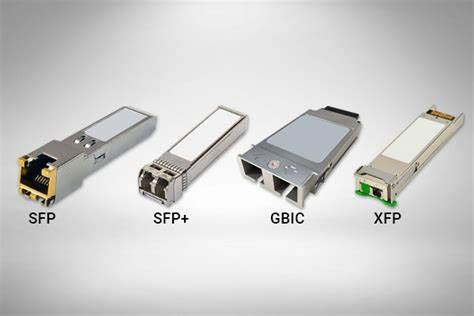
\includegraphics{images/sfp.jpeg}
      \caption{SFP transceivers form factors}
      \label{fig:sfp}
   \end{figure}
\end{paracol}

\note{Fun fact: ci sono 9 cavi USB-C e solo due portano informazioni video.}

\subsubsection{Issues about cabling and fabric}
The key point is that it would be desirable for cabling to be reconfigurable, that's why transceivers are so important.

\note{There are things called \textit{``Muffole''}, which are used for joining optical fiber cables, allowing for longer distances to be covered.
They are designed to be underground.}

Data traffic is always at least SFP+.
Current standard is SFP28. Various SFP are typically compatible, the shape of the plug should stay the same.
On switches there also some ports which are \texttt{QSFP+} or \texttt{QSFP28}, which allow up to \texttt{40} and \texttt{100Gbit/s} respecitively, and are used for north-south traffic.
\note{The \texttt{Q} letter stands for \textit{Quality}}

Switches for datacenters should be \textbf{non-blocking}, meaning that no port has to wait for other ones ---or any other thing--- before transmitting, they can also transmit simultaneously.


\ul{In every datacenter it is \textit{MANDATORY} to document the cabling.}

\subsection{InfiniBand}
Even though Ethernet is famous, it is not the only standard. InfiniBand is another one, which is used in supercomputers and known for its very high throughput and very low latency ($\sim 2\mu s$).
It may send messages up to 2GB each, with 16 priority levels.
It is a \textit{lossless protocol}, meaning that if a packet is received, its integrity is guaranteed.

\textit{IB} avoids TCP/IP stack, which is very heavy, and instead uses MPI (\textit{Message Passing Interface}), which is a way to distributed parallel programs, also exploited by OmniPath.

InfiniBand cables and connectors look similar to Ethernet ones, but they are not compatible.

Aside from HPC environments, it is uncommon to build an entire network with InfiniBand, typically there is an IB switch to whom the servers equipped with IB NICs are connected, which intereacts with the rest of the network with Ethernet, because ``it's cheaper and it works''.
\note{Today, we are about 400 Gbit/s on both IB and Ethernet.}

\subsection{RDMA - Remote Direct Memory Access}

RDMA is a technology API based (not a protocol!) that allows to access memory of a remote machine without involving the CPU or the OS of the remote machine.

RDMA supports zero-copy networking by enabling the network adapter to transfer data directly to or from application memory, eliminating the need to copy data between application memory and the data buffers in the operating system.\\
The main use case is distributed storage.

RoCE (\textit{RDMA over Converged Ethernet}) is a network protocol that allows remote direct memory access (RDMA) over an Ethernet network.

\subsection{Omni-Path}
Omni-Path is a high-performance computing network architecture, developed by Intel. It is a successor to Intel's InfiniBand, and competes with InfiniBand's EDR and HDR technologies.

Intel plans to develop technology that will serve as the on-ramp to \textit{exascale computing}\footnote{A computing system capable of the least one exaFLOPS}, which is the next frontier in high-performance computing.


\chapter{BitTorrent}

The goal of \textit{Content Distribution Networks} is to distribute web contents to hundreds of thousands or millions
of simultaneous users, \ul{exploiting data and/or service \textbf{replication} on different \textbf{mirror servers}}.

In \textbf{P2P CDN} the initial file request are served by a centralized server, and further requests served by peers which have already received and replicated the files (\textbf{\textit{seeders}}), without involving the initial server.

\begin{center}
\fbox{
   \begin{minipage}{0.8\columnwidth}
      \nl
      \begin{center}
         \ul{\textbf{BitTorrent} in a nutshell}
      \end{center}
      \nl

      \begin{itemize}
         \item Basically a \textit{Content Distribution Network} (\texttt{CDN})
         \item A distributed set of hosts cooperating to distribute large data set to end users.
         \item Efficient content distribution systems using \textit{file swarming}
         \item Does \textit{not} perform all the functions of a typical P2P system, like searching
         \item Rather than providing a search protocol itself, was designed to integrate seamlessly with the Web and made file descriptors available via Web, which could be searched with standard Web search
         \item \textit{File swarming}: a peer makes whatever portion of the file that is downloaded immediately available for sharing
      \end{itemize}
   \end{minipage}  
   }
\end{center}

\section{Deeper into BitTorrent}
\begin{figure}[htbp]
   \centering
   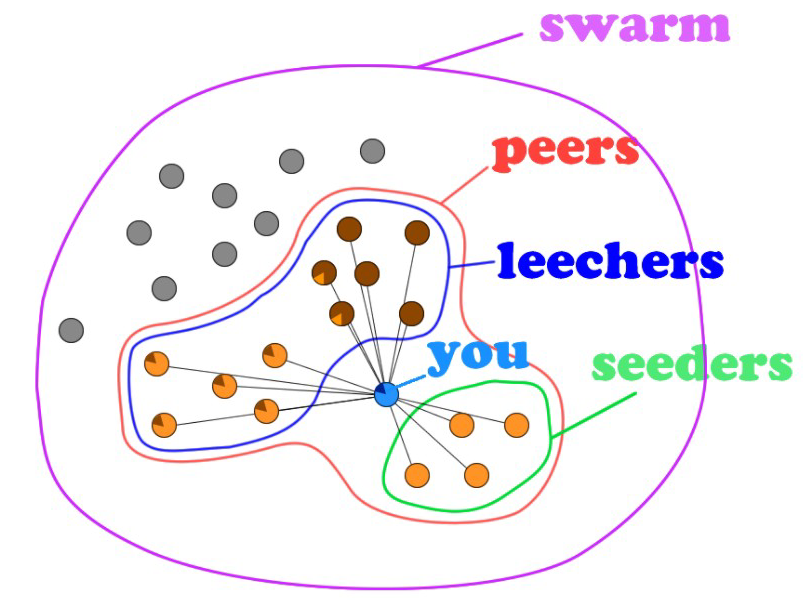
\includegraphics{images/bit_swarmschema.png}
   \caption{Swarm schema}
   \label{fig:bit_swarmschema}
\end{figure}
\subsection{Glossary}
\begin{itemize}
   \item \textbf{tracker}: active entity which coordinates
   the peers sharing the file, taking trace of who is currently providing the content
   \note{\begin{itemize}
      \item Joe connects to the tracker announcing the content
      \item the tracker now knows Joe is providing the file
   \end{itemize}}
   \item \texttt{.torrent} a descriptor of the file to be published on a server, which includes a reference to a tracker
   \item \textbf{swarm} set of peers collaborating to the distribution of the same file coordinated by the same tracker
   \item \textbf{seeder} peer which owns all the parts of the file
   \item \textbf{leecher} peer which has some part or no part of the file and downloads the file from the seeders and/or from other lechers.
\end{itemize}

\subsection{Protocol Overview}
\begin{figure}[htbp]
   \centering
   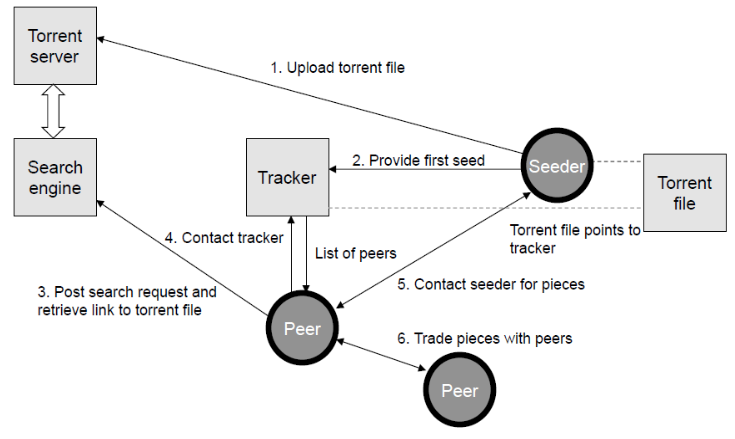
\includegraphics{images/bit_overview.png}
   \caption{BitTorrent protocol overview}
   \label{fig:bit_overview}
   BitTorrent protocol is built on top of HTTP
\end{figure}
\labelitemize{\textit{Seeder}}{
   \begin{enumerate}
      \item Upload the .torrent on a Torrent Server
      \item Opens a connection to the Tracker and informs it of its own existence: for the moment, it is the only peer which owns the file
   \end{enumerate}
}
\labelitemize{\textit{Peers}}{
   \begin{enumerate}
      \setcounter{enumi}{2}
      \item Retrieves the file descriptor (.torrent) and opens it through the BitTorrent
      client
      \item Opens a connection to the tracker and informs it of its own existence and
      receives from the tracker a list of peers of the swarm
      \item Opens a set of connections with other peers of the swarm.
   \end{enumerate}
}

Objects are serialized in \textbf{Bencode}, which is ---not popular as \texttt{JSON}--- used only in torrent; provides 4 data types: String, Integer, Lists and Dictionaries.\\
Content is split into chunks called pieces (256KB - 2MB):
when a peer receives a piece, it becomes the seeder of that piece.
\note{
   \ns
      There is a SHA-1 hash per piece stored in the .torrent file, used to check the piece once it is fully downloaded, 
      allowing to require retransmission in case the check fails.\\
      Pieces size got adapted to have a reasonably small .torrent file
}
Pieces are then split in \textbf{subpieces} (\textit{\textbf{blocks}}) of 16KB, with each one downloadable from a different peer, optimizing the bandwith and allowing \textit{pipelining}, decreasing the overall download time.

Trackers keep a database of swarms identified by torrent hash, and knows also the state of each peer in each swarm.
In the last versions, \textbf{trackerless} BitTorrent uses \textit{Kademlia DHT} to avoid the centralization point of the tracker.

\section{Pieces selection}
The order in which pieces are selected by different peers is critical for good performance, to avoid making peers end up stuck with the same pieces.
\labelitemize{\textit{Policies}}{
   \begin{itemize}
      \item \textbf{Strict Priority}\\
      Complete the ``assembling'' of a piece before asking for another piece
      \item \textbf{Rarest First}\\
      Download the rarest pieces first
      \item \textbf{Random First Piece}\\
      Choose a random piece ---only--- in the bootstrap phase
      \item \textbf{Endgame}\\
      When the file download is almost terminated, the remaining pieces are required in \textit{parallel} to all peers who own them.
      This policy is executed for a small period of time
   \end{itemize}
}

\subsection{Free Riders}
Free riders in BitTorrent are peers that do not put their bandwidth at disposal of the community.\\
Several non official BitTorrent clients enable the user to limit the upload bandwidth as they like.

However, an approach to solve this problem is based on \textbf{reciprocity}, allowing a client to obtain a good service if and only if it gives a good service to the community, by exploiting a dynamic strategy based on connection monitoring called ``Tit for Tat'', implemented using \textbf{choking}:\\
choking means \textit{temporarily} refusing to upload to another peer, but still downloading from them;  
the principle is to upload to peers who have uploaded to us.

\labelitemize{\textit{Choking}}{
\begin{center}
   \textit{The local peer can receive data from a remote peer if}
   \begin{itemize}
      \item The local peer is \textit{interested} in the remote peer
      \item The remote peer \textit{unchoked} the local peer
   \end{itemize}
\end{center}
   }

Choking only peers that upload the most to the local peers would lead to ignoring peers that recently join the network
and to the lack of discovery of connections actually better than the used ones.\\
To avoid this, BitTorrent uses \textbf{optimistic unchoking}, i.e. \ul{one random peer is being unchoked}.\\
Then, every 30s an interested and choked peer is selected at random \textbf{planned optimistic unchoke} (\texttt{POU}), and if this new connection turns out to be better than one of the existing
unchoked connections, it will replace it.

In case a peer is chocked by everyone, it follows an \textbf{anti-snubbing} policy, by increasing the number of simultaneous optimistic
unchocke to more than one.

For \textit{seeders} this schema does clearly not apply, since they do not have to download anything; hence they use a different choking algorithm:
\ul{unchoke peers with the highest upload rate}, ensuring that pieces get uploaded and replicated faster.

\section{DHT and BitTorrent}
Kademlia is the protocol used by the largest public DHTs.
Bittorrent Inc. introduces its own DHT, called \textit{Mainline DHT}.
With respect to Kademlia there are some improvements concerning 
\begin{itemize}
   \item Routing table management
   \item Look-up
\end{itemize}

The main purpose of Mainline DHT is to provide a “trackerless” peer discovery mechanism to locate peers belonging to a swarm.
\chapter{Storage}

\framedt{Data Loss}{
   \textit{``Storage is crucial because, if a switch fails, or a server fails, the service will be interrupted, but the data will still be there. \ul{If the storage fails, the \textbf{data will be lost}}.''}
   -Prof. Cisternino\\

   \textbf{Data} is the most important of a system. Since data loss is \textbf{permanent}, the storage is completely different from computing or networking.
}

\begin{paracol}{2}
   \colfill
   Historically the storage was the slowest part of the system, \textit{ms} against \textit{ns} of the CPU.
   Today, with SSDs, the gap is considerably reduced to \textit{$\mu s$}, they are $\sim 100x$ times faster.
   
   \ul{NVMe stands for \textit{Non-Volatile Memory Express}, and is a protocol (\textit{not a HW component!})} that allows to access the storage directly from the PCIe bus, without having to go through the SATA controller. This allows to have a much higher throughput, and a much lower latency.

   \note{Optane was a technology developed by intel which is now end of life}

   \colfill
   \switchcolumn

   \begin{figure}[htbp]
      \centering
      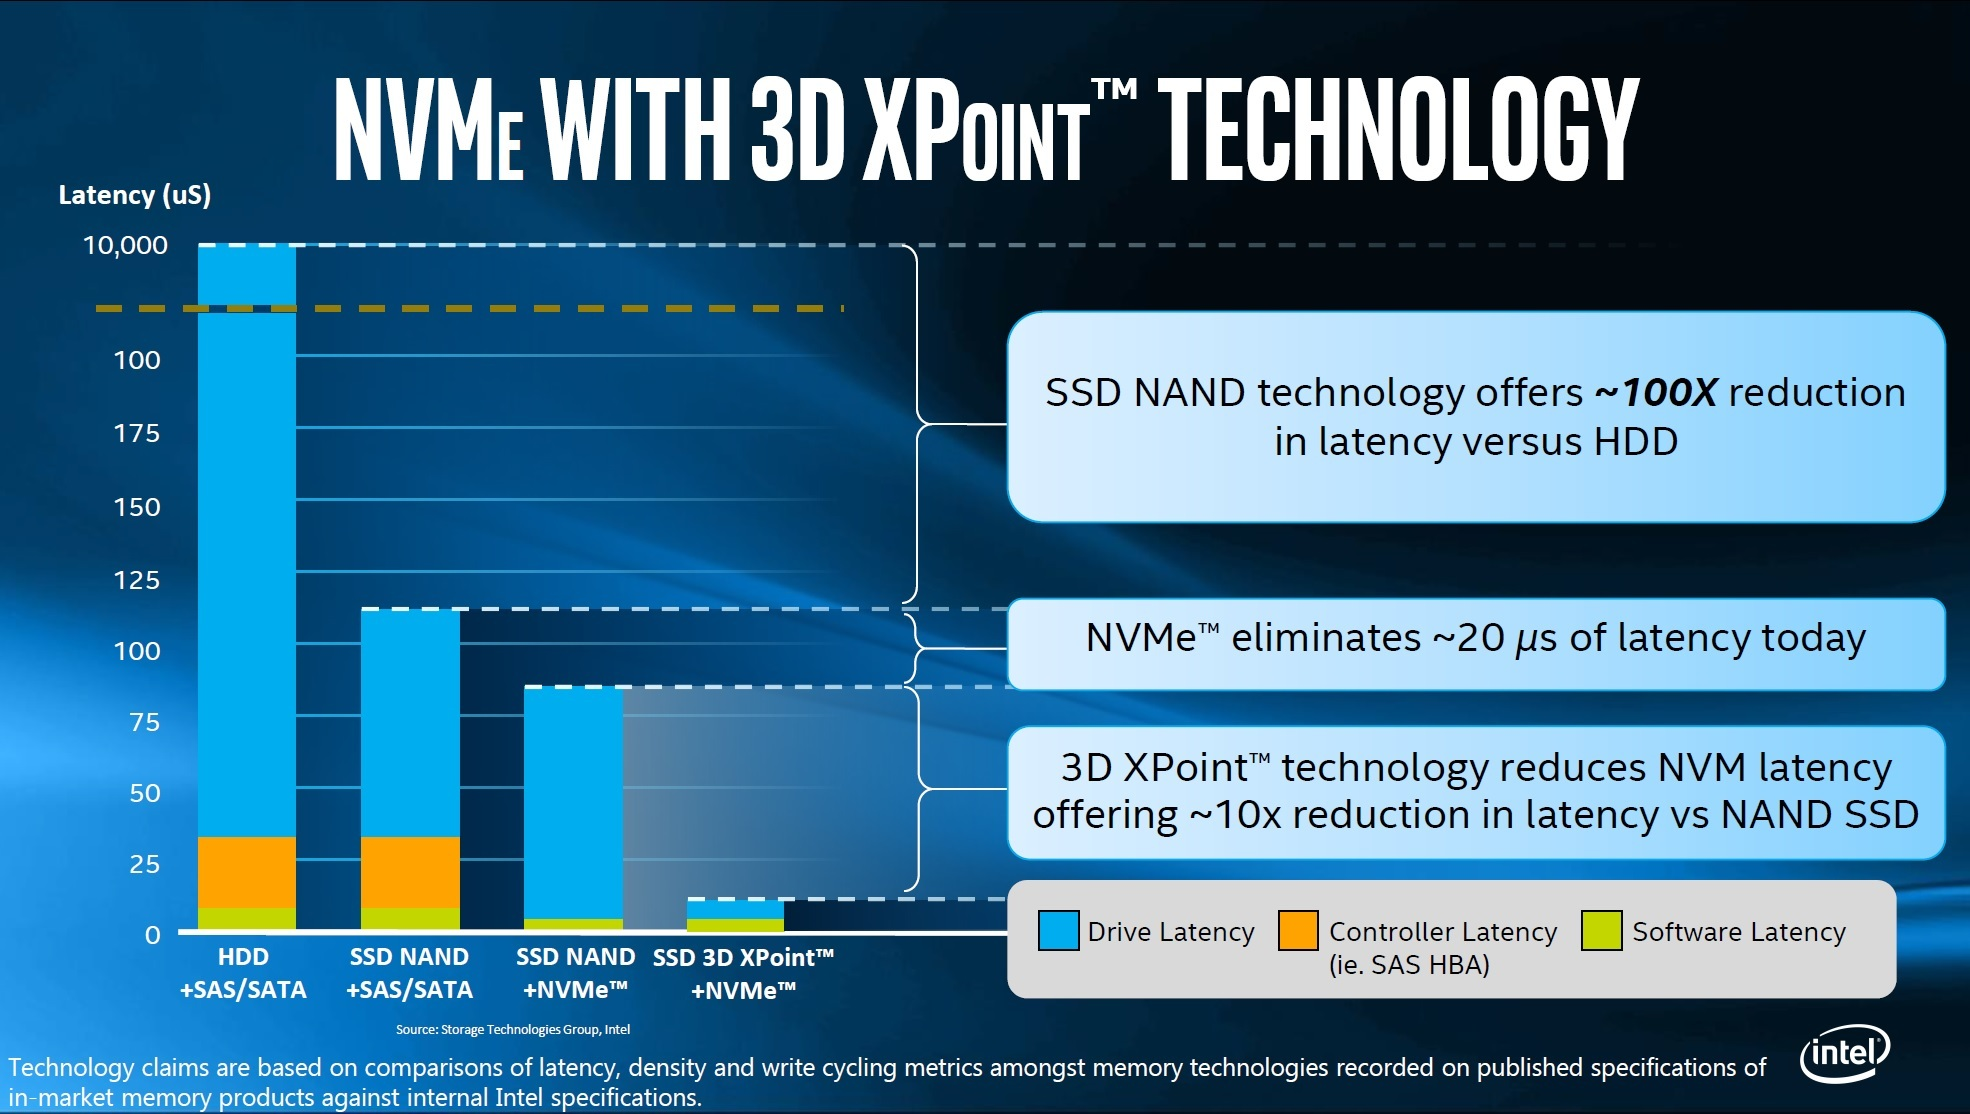
\includegraphics{images/storage_intel.jpg}
      \caption{Storage types comparison}
      \label{fig:storage_intel}
      NVMe basically removes the orange part of the figure, which is the latency introduced by the controller, since it is a \textit{controller-less protocol} and allows to access the storage directly from the PCIe bus.
   \end{figure}
\end{paracol}


\framedt{
   \textit{Why would a 15TB disk be better than a 27TB disk?}\\
   }{
      \note{Assume the same performance, and the same price.}
      It would be preferrable because \ul{it would take less time to extract all the data from the disk}\footnotemark[1], since it is smaller.
      
      However, large capacity drives are used for \textit{cold storage}, where the data is not accessed frequently, speed is not a priority, and even if the data is accessed, only a portion of the disk is needed at a time; in case of failure and thus needing to retrieve an entire backup, the time taken to retrieve the data is not a priority, since this ---hopefully--- happens only ``once''.
      }
      
\footnotetext[1]{i.e. taking advantage of the space provided}
\section{SSDs - QLC and TLC}
SSDs were invented by Toshiba back in 1980, but they were not popular for almost 30 years, until they eventually became cost-effective. Sometimes extra size in SSDs is used for redundancy, to increase the lifespan of the disk e.g. on a 30TB disk, only 10TB are used, the rest is used for redundancy, extending x3 the lifespan of the disk.

\note{DWPD stands for \textit{Drive Writes Per Day}, and is a measure of how many times the disk can be written to in a day. It can be calculated as $\frac{TBW}{365\times\textit{Years of Warranty}\times\textit{capacity}}$}.

TLC stands for \textit{Triple Level Cell}, and QLC stands for \textit{Quad Level Cell}. The difference between the two is the number of bits stored in each cell. The more bits stored in each cell, the cheaper the disk is, but the slower it is. The more bits stored in each cell, the more difficult it is to read and write the data, and the more difficult it is to keep the data stored in the cell.

Generally QLC disks are used for cold storage, while TLC disks are used for hot storage.
TLC in general is more reliable than QLC, has a longer lifespan and better performance, however they cost more.

\section{Storage Concepts}
\subsection{Tiering - Memory Hierarchy}

\begin{figure}[htbp]
   \centering
   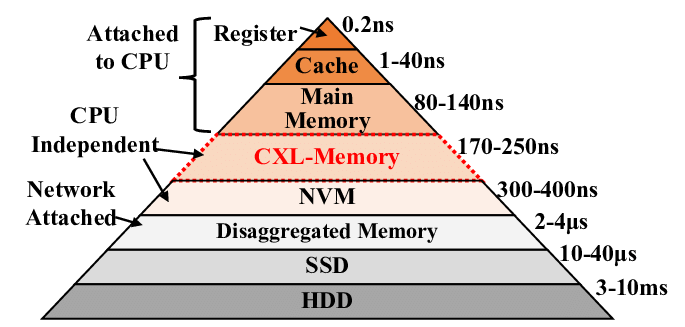
\includegraphics{images/tiering_memory.png}
   \caption{Memory tiering hierarchy}
   Ram could actually be split in \texttt{RAM} and \texttt{nvRAM} (Non-volatile \texttt{RAM}, uses \texttt{nvDIMM}), which is used to store the data in case of a power failure.
   Sometimes, \textit{tape} is included in the hierarchy, because it is used for long-term storage, and it is very cheap.
   \label{fig:tiering_memory}
\end{figure}

Tiering consists in categorizing the data in different categories, and storing the data in different types of storage, depending on the category. The data that is accessed more frequently is stored in the fastest storage, while the data that is accessed less frequently is stored in the slowest storage. This allows to increase the performance, and to reduce the cost. 

\subsection{IO operations, are they all the same?}
\textbf{IOPS} (Input/output operations per second) is an input/output
performance metric used to characterize computer storage devices; it is associated with an access pattern: \textit{random} or \textit{sequential}.

\subsubsection{Random vs Sequential access}

Before explaining the distinction, is important to remember the concept of \textit{queues}: for each thread, the OS can implement a series of queues to solve asynchronously the I/O requests. Using multiple queue can make performances better, since having
the OS to manage parallel requests will increase throughput.
If the queries are latency sensible, not using a queue is better, since
it allows a single query to have ``max'' priority.

\textit{Random access files} are advantageous in scenarios where frequent direct access or modification of specific records is required, while \textit{sequential access files} are advantageous in scenarios where frequent reads of the full files are required. The disk behaves differntly in case of access of those files.

To have a full picture of random vs sequential access, check this site: \url{https://www.prepbytes.com/blog/general/difference-between-sequential-and-random-access-file/} 

\newpage
\subsubsection{Cisternino's demo}
Prof. Cisternino showed a demo in class, where he used a tool to measure the IOPS of a disk.
\begin{figure}[htbp]
   \centering
   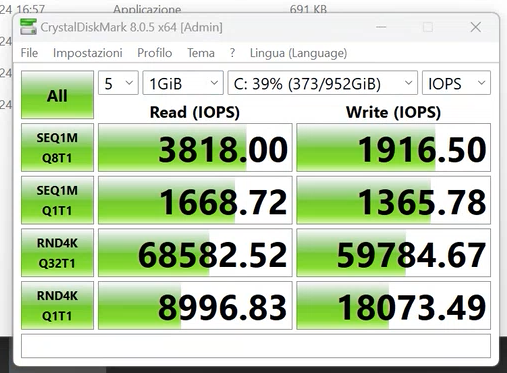
\includegraphics{images/iops.png}
   \caption{IOPS demo; respetively}
   \label{fig:iops}
\end{figure}

\ul{Recall that IOPS by itself is meaningless!} It is a number that must qualified and put in relationship with something else.

\subsection{Latency and Storage Aggregation}
A mechanical hard drive introduces 2.71\% of latency when reading, for instance, 40MB of data.  Optane can perform 416 accesses in the same time needed by a mechanical hard drive to perform 1 access. It looks like the latency in this latter case is neglegtible. Someone may be tempted to reduce the size of read/write operations and perform multiple smaller ones, since ``it's free''. 

Latency in general is due to:
\begin{itemize}
   \item \textbf{Software}\\
   $\mu s$ order which cannot be removed
   \item \textbf{Controller}\\
   Taken down to $20\mu s$ with NVMe (even $2.8\mu s$ according to Copilot)
   \item \textbf{HDD latency}\\
   This was drastically reduced with SSDs and got even less with 3D NAND.
\end{itemize}
Latency may be solved by \textbf{storage aggregation}, which consists in aggregating multiple storage devices into a single logical unit, in order to increase the performance and reliability.
Even if the data is split in multiple disks, the whole system is ``pictured'' as a single huge drive\footnote{\textit{``Cloud resource pooling''} rings a bell?}, making a huge difference in terms of latency, since multiple \texttt{read/write} requests may be sent in parallel to multiple disks.

\newpage
\subsection{Storage Fabric - Fibre Channel}
\textbf{Fibre Channel} is the fabric dedicated to storage; the link coming from the storage ends up in the \textit{HBA} (Host Bus Adapter) in the server.
\begin{paracol}{2}

   \colfill
   The idea is to have an interface which announces itself as drive and that manages the remote storage through Fibre Channel.
   Fibre Channel typically runs on optical fiber cables, but may also run on Ethernet cables (FCoE).

   In Fig. \ref{fig:fibrechannel} is depicted the ideal architecture for Fibre Channel, where the storage is connected to the network through a switch, and the servers have a dedicated HBA to connect to the storage.
   \colfill
   
   \switchcolumn
   \begin{figure}[htbp]
      \centering
      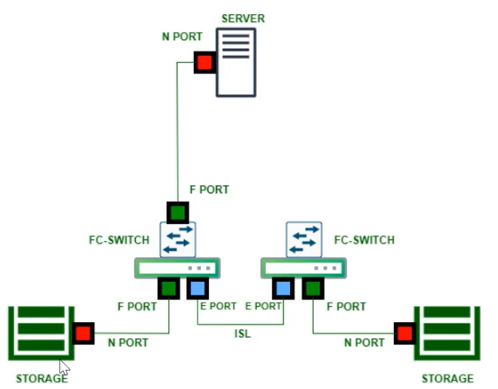
\includegraphics{images/fibrechannel.png}
      \caption{Fibre Channel desired architecture}
      \label{fig:fibrechannel}
   \end{figure}
   
\end{paracol}

\begin{figure}[htbp]
   \centering
   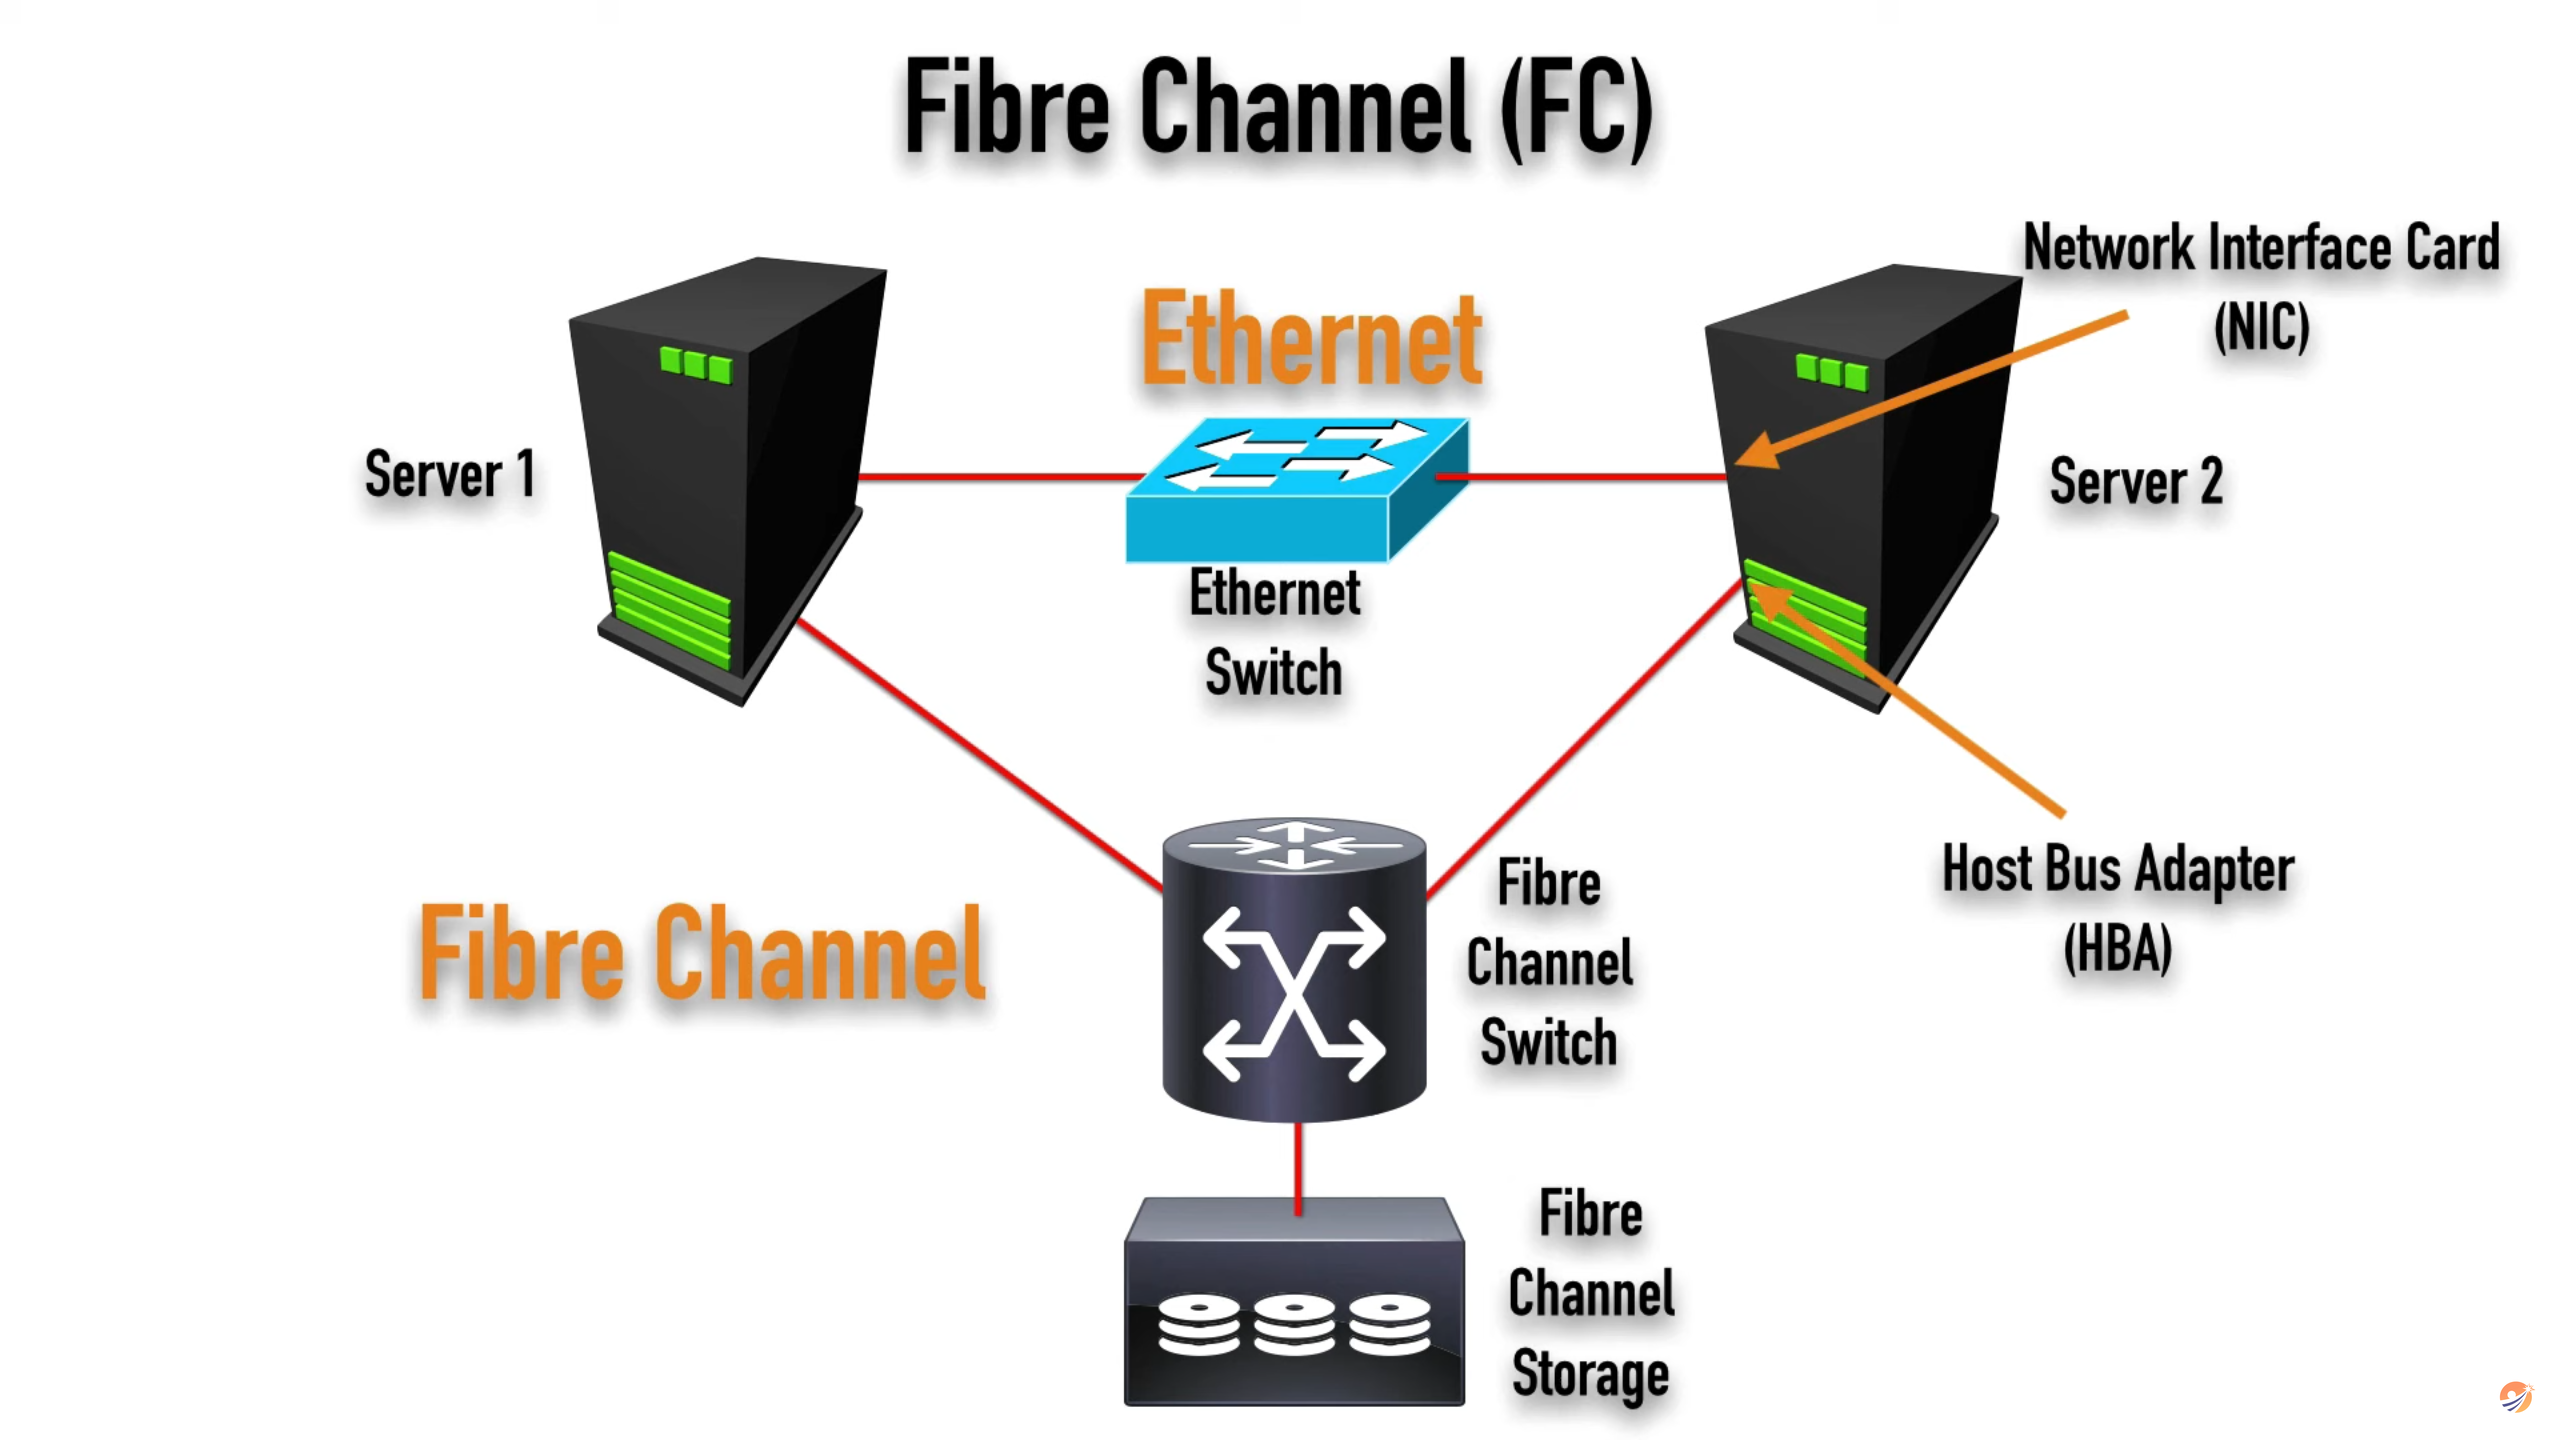
\includegraphics[width=0.32\columnwidth]{images/storage_fabric1.png}
   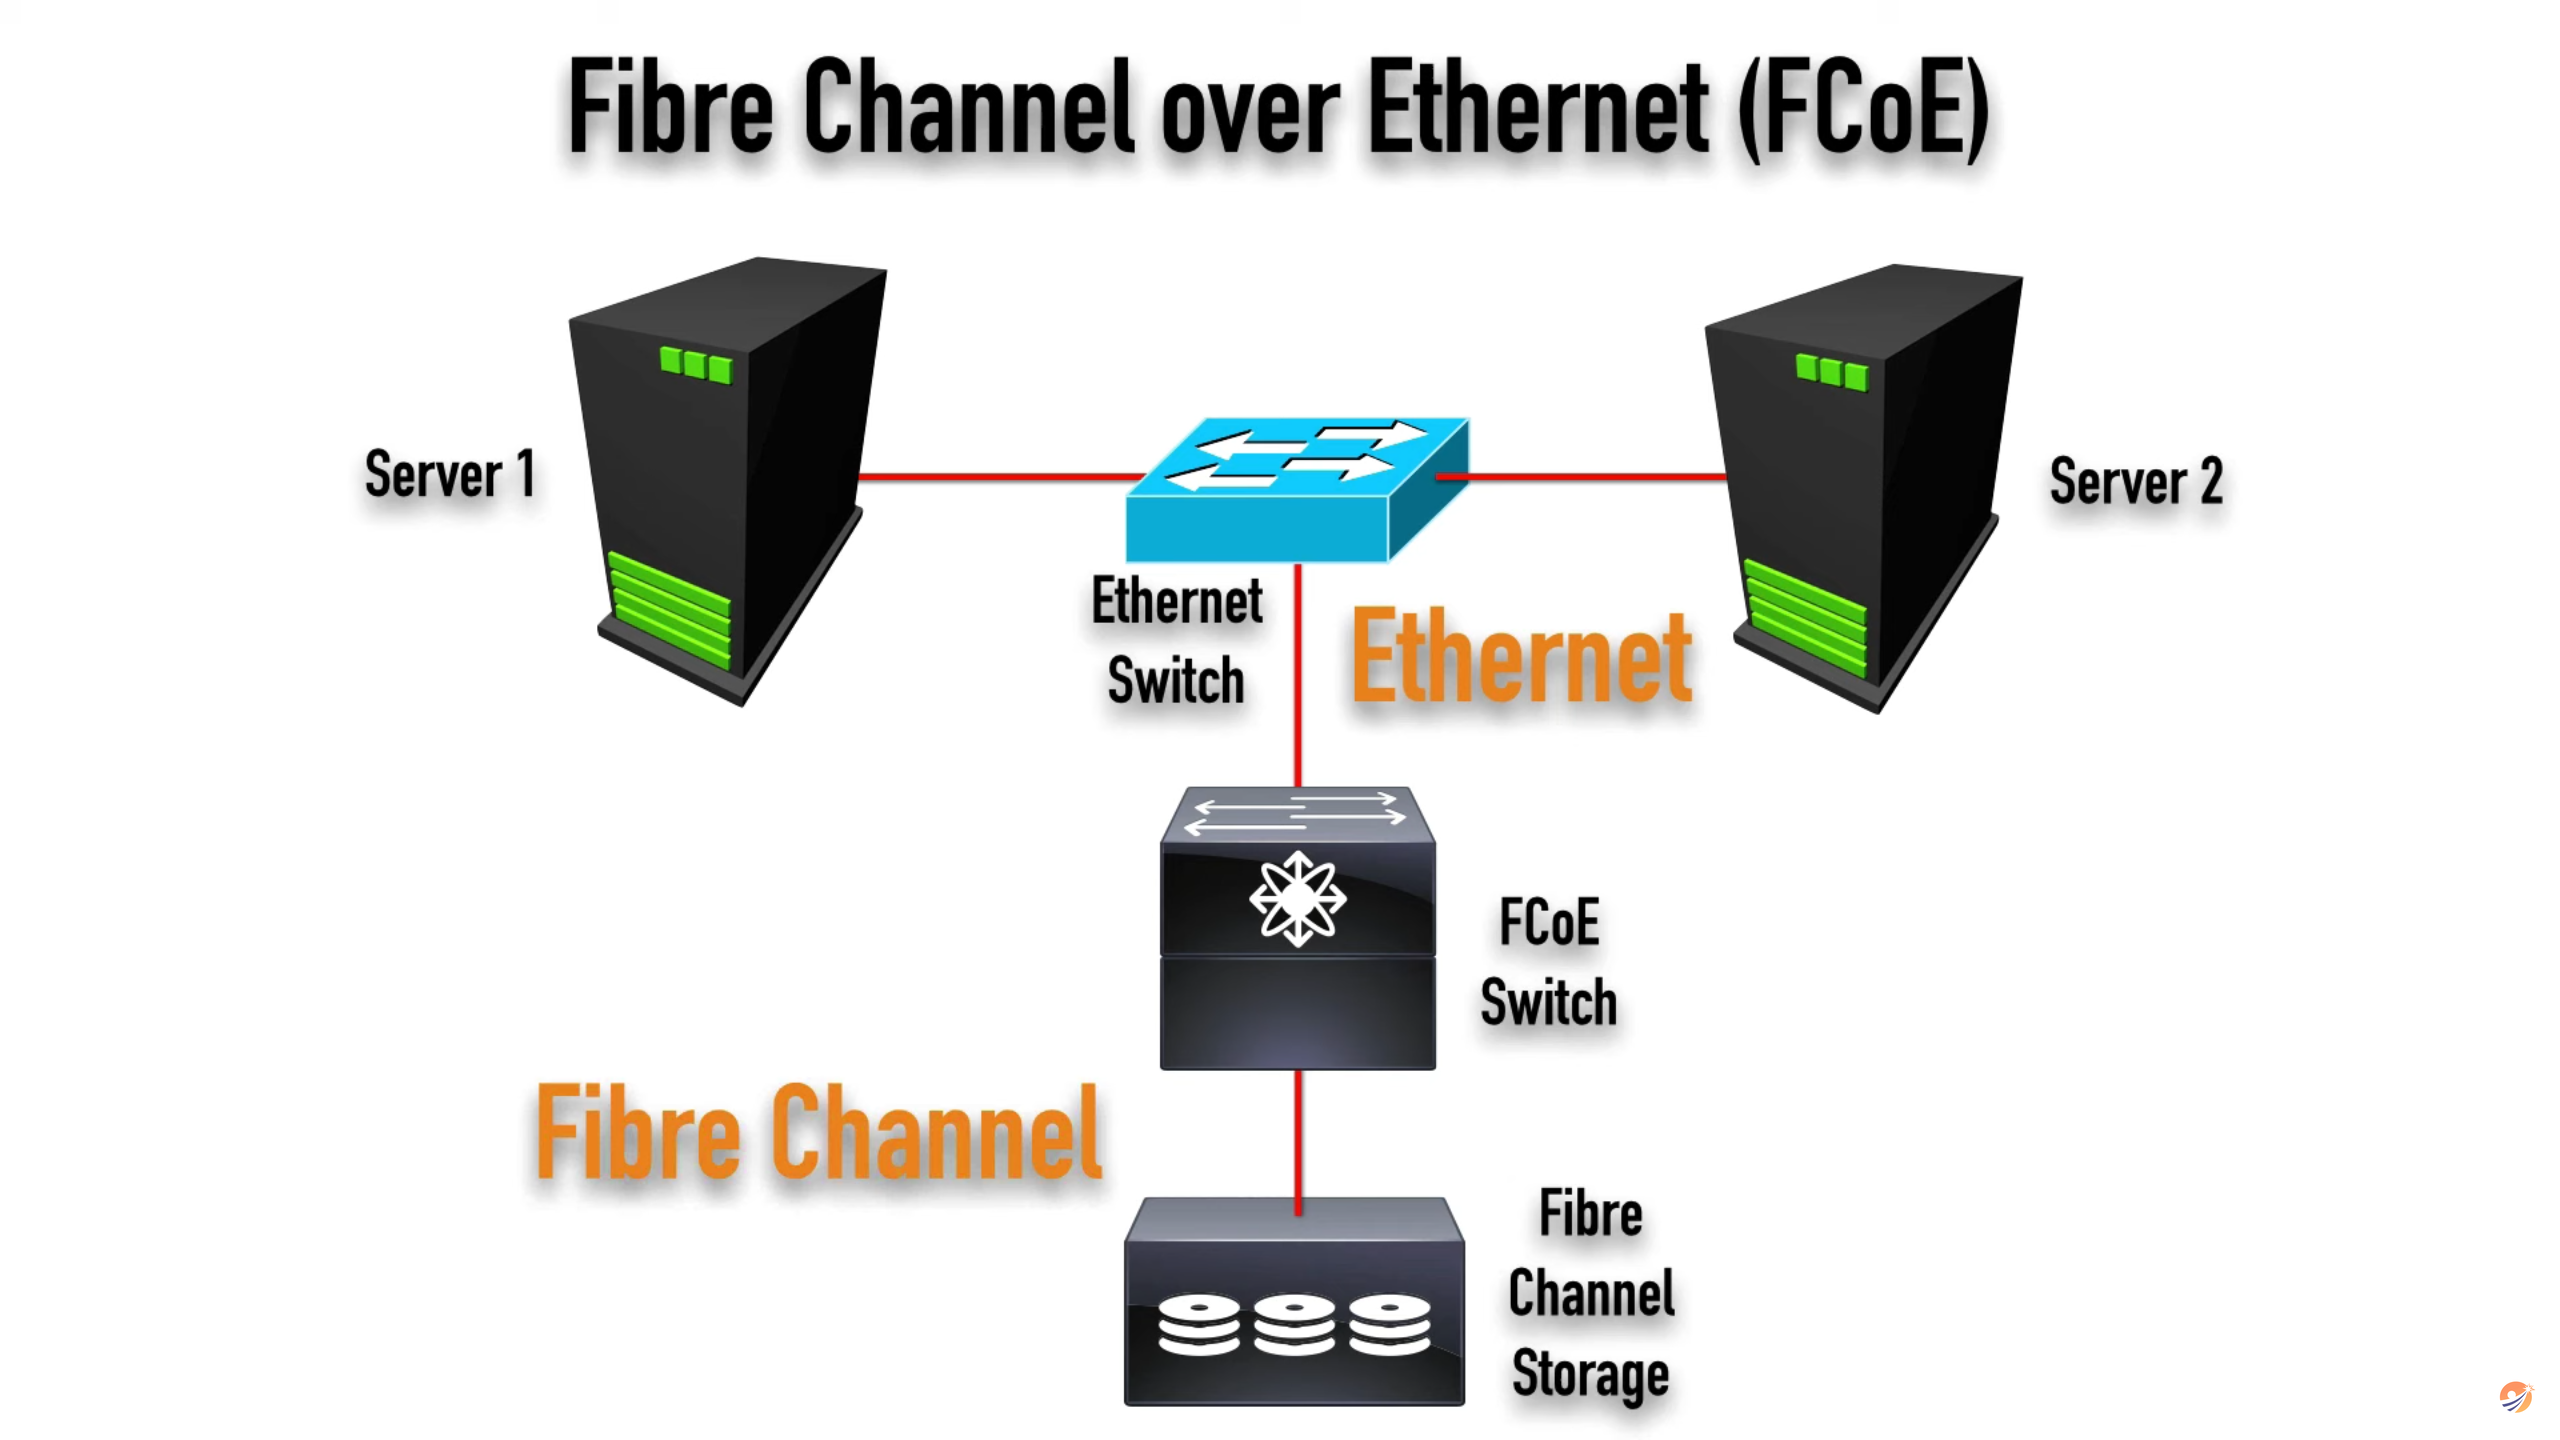
\includegraphics[width=0.32\columnwidth]{images/storage_fabric2.png}
   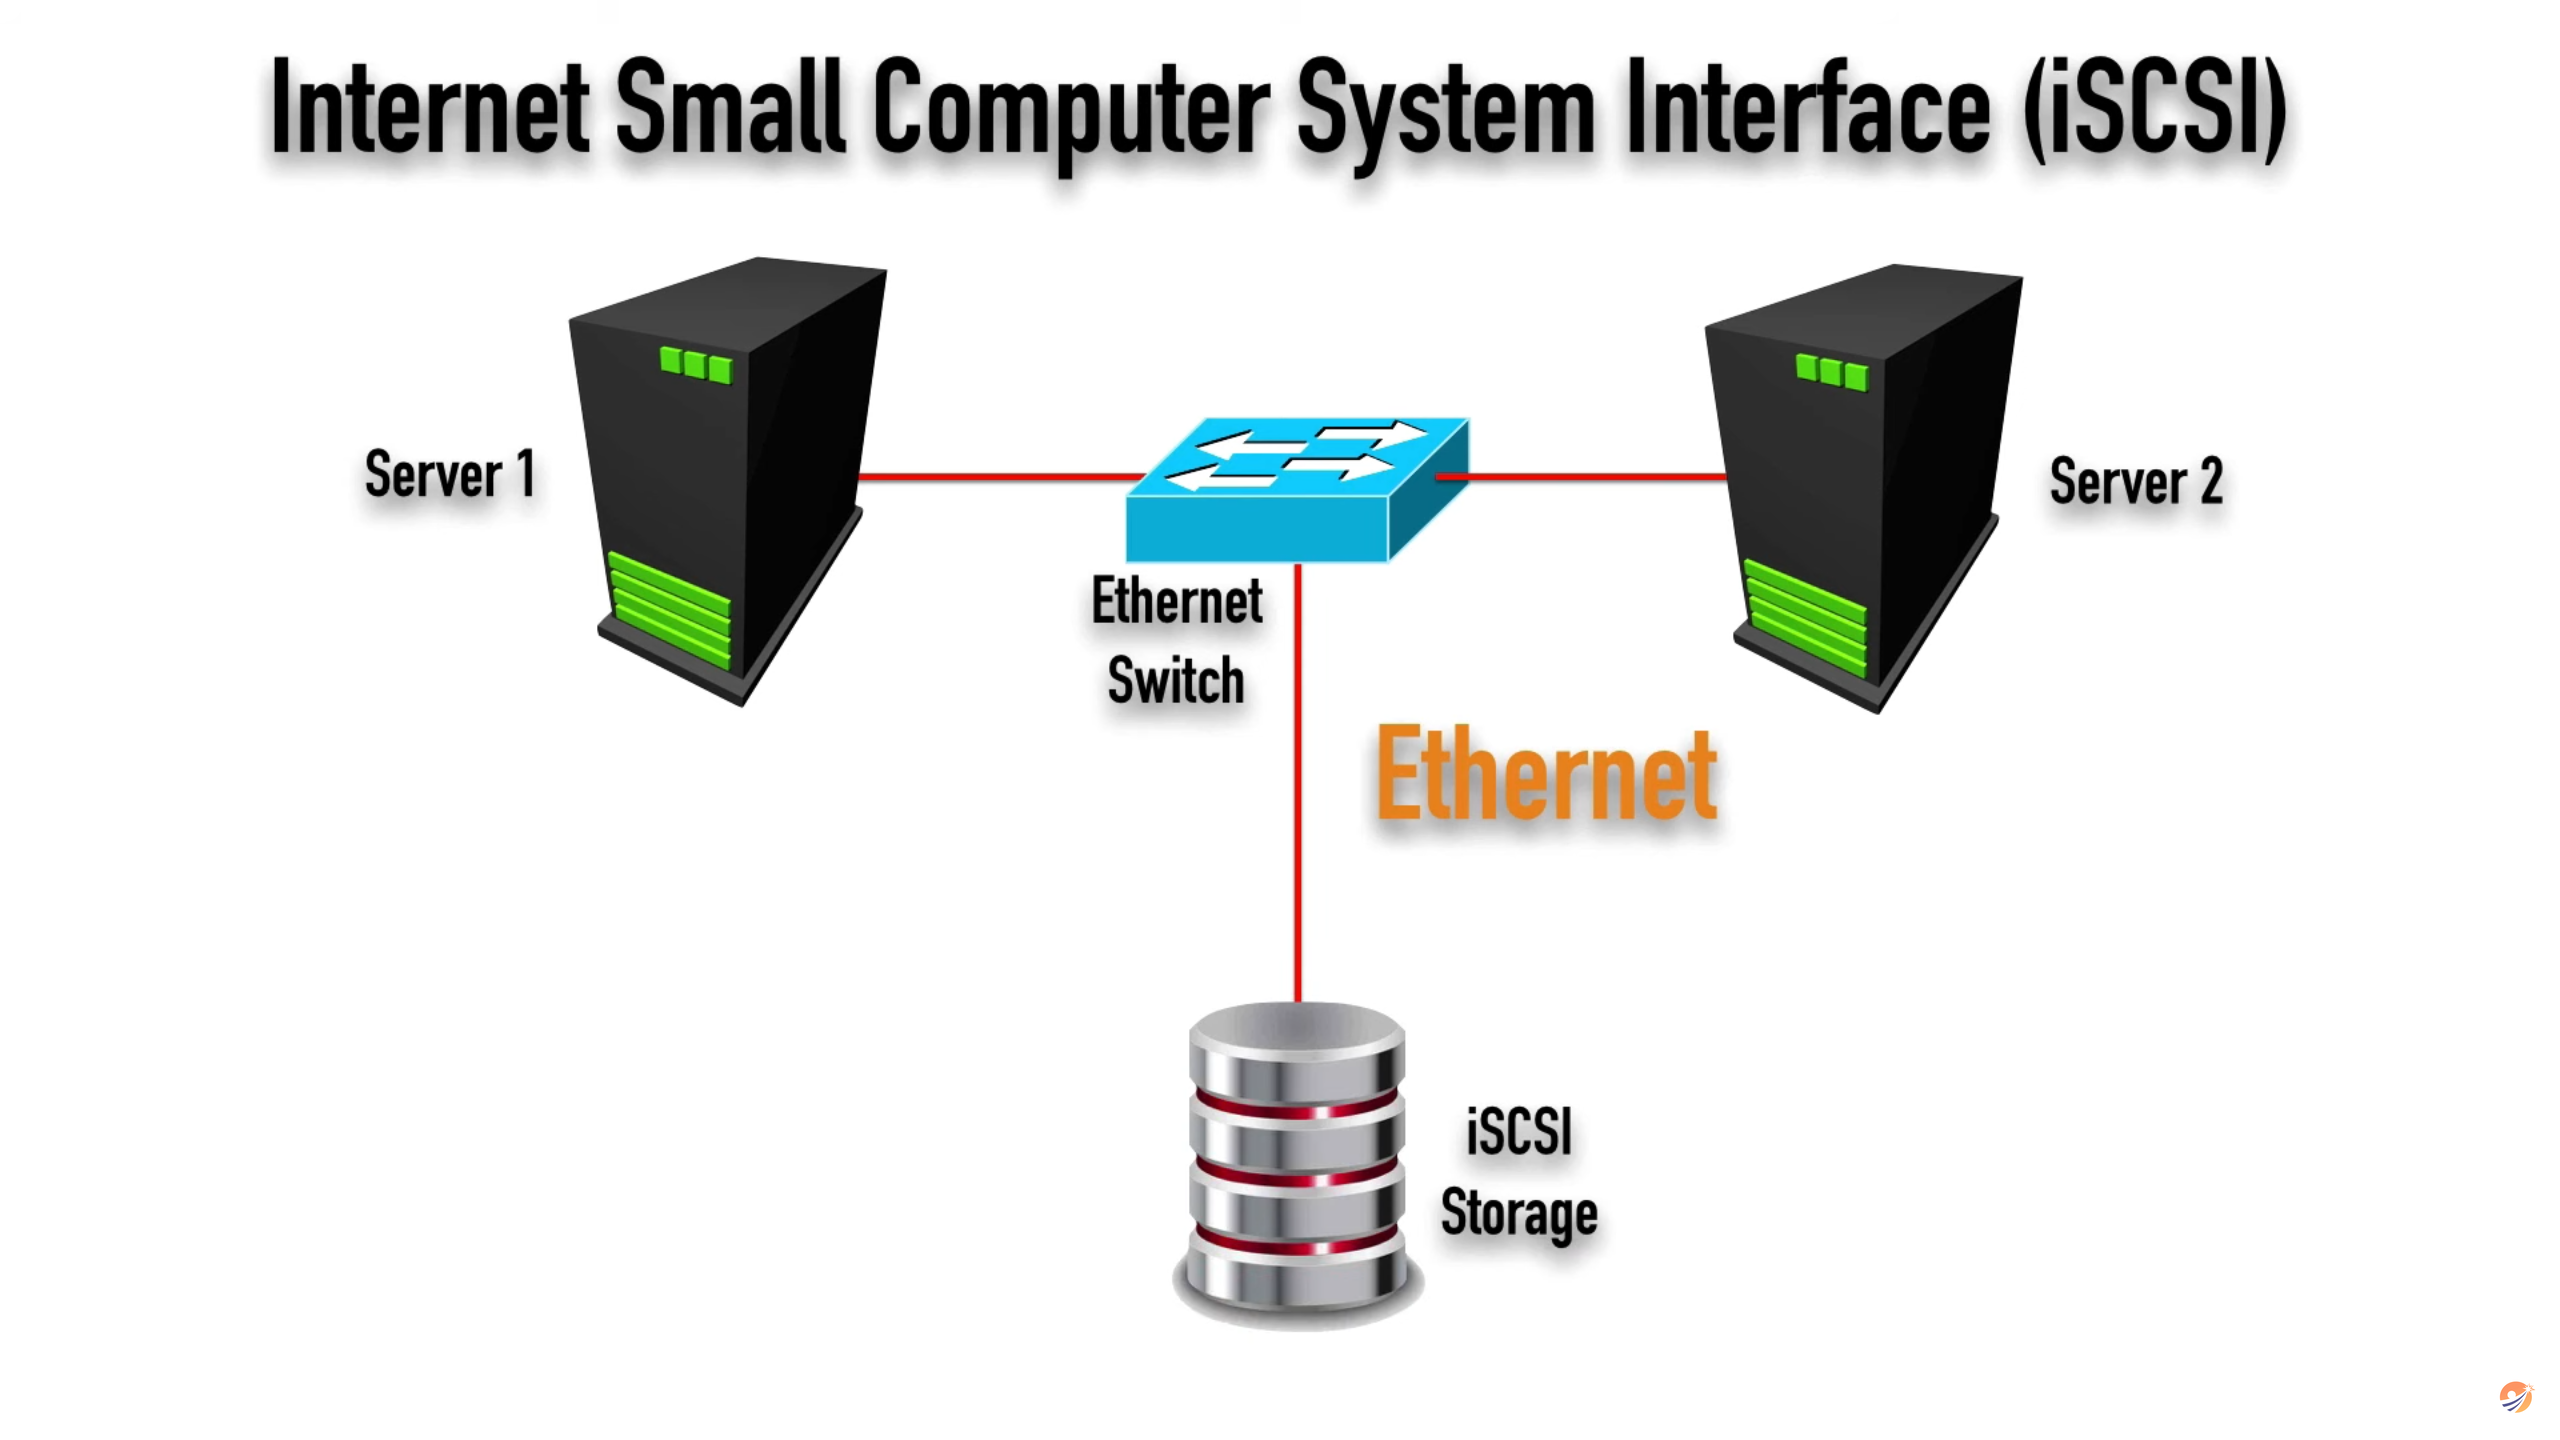
\includegraphics[width=0.32\columnwidth]{images/storage_fabric3.png}
   \caption{These are three possible configurations for the storage fabric, the first being the most performant, and the third being the cheapest.
   Note that in the second picture the first link is Ethernet and the second is Fibre Channel.}
   \label{fig:storage_fabric}
\end{figure}
Note that the image may me misleading, since there may be multiple FC switches (as partially depicted in Fig. \ref{fig:fibrechannel}) and multiple storage racks.
   
\subsection{Bus, controller and some numbers}
A bus is a component to whom multiple devices may be attached. It has a clock and some lanes, 16 in the case of PCI, each one providing almost 1GB bandwidth, summing up to $\sim 15GB$: 4 drives are enough to saturate a full PCI bus, or a 100Gbit link ($12.5GB/s$).;
in fact an NVMe SSD has a bandwidth of 3.5GB/s, hence $3.5\times 4 = 14GB/s \simeq 15GB/s$.\\
NVMe is often used in the lower memory tier of the RAM: its speed is only one order of magnitude less than RAM, but can provide high capacity without any problem.
It may represent a valid super-fast cache level for the RAM and hence started being associated in one single level to implement a big RAM tier, in a totally transparent way for the system.

Since the software latency in disk IOs is 5 microseconds more or less,
TCP/IP software introduces also a latency of 70-80 microseconds, the disk is
no more a problem. Indeed, the problem is now the network, not only for the
latency, but also for the bandwidth: as stated before 4 NVMe totally saturate a 100 Gbps
link.

\section{Redundancy and backup}
\subsection{Checkpoints}
It's unpractical for a system to go down after 5 months. For this reason it is necessary to have \ul{\textit{checkpoints}, which are points in time where the system can be restored to.} The system can be restored to the last checkpoint, and the data that was written after the checkpoint can be re-applied. This is similar to what happens to applications on smartphones are closed and then re-opened, the application is restored to the last checkpoint.

\subsection{RAID}
\textbf{RAID} stands for \textit{Redundant Array of Independent Disks}. It is a technology that allows to combine multiple disks into a single logical unit, in order to increase the performance, the reliability, or both. There are different levels of RAID, each with different characteristics.

Historically \textit{Redundant Array of Inexpensive Disks}, because it was more common for disks to eventually fail, so RAID was the only countermeasure to this. Today, disks are more reliable, so RAID is used more for performance reasons.

In RAID, \textbf{XOR} is used to calculate the parity of the data. The parity is used to recover the data in case of a disk failure. The parity is calculated by XORing the data of the disks. The parity is stored on a separate disk, called the parity disk. The parity disk is used to recover the data in case of a disk failure.


\section{Network sharing architectures}
Before going into the details of the architectures, it is important to understand the difference between \textbf{protocols} and \textbf{architectures}.\\
\textbf{SMB/CIFS} is a protocol that allows to share files over the network. It is used by Windows, but it is also supported by Linux and MacOS. NFS is a protocol that allows to share files over the network, it is used by Linux and MacOS, but it is also supported by Windows.\\
NFS is faster than SMB, but it is also less secure. SMB is slower than NFS, but it is also more secure.\\
These however are protocols for file sharing, not properly ``architectures''.

\framedt{Capacity and system architecture}{
   When we talk about \textbf{capacity}, there are two measures which we can refer to:
   \begin{enumerate}
      \item \textit{Scale-\textbf{up}}:
      adding more disks to the same server
      \item \textit{Scale-\textbf{out}}:
      adding more servers to the same network
   \end{enumerate}
}

\subsection{File based - NAS}
\textbf{NAS} are devices that are connected to the network, and that are used to store files, providing aggregated capacity. They are used to store files that are accessed by multiple users, and that need to be accessed from multiple devices.
NAS systems have integrated HW and SW component, including CPU, memory, NICs, optimized OS for file serving, file sharing protocols and so on.\\
Typically they exploit SMB/CIFS or NFS protocols, or AFP over optical fiber, and represent a good solution for \textit{document management}.

\subsection{Block based - SAN}
\textbf{SAN} stands for \textit{Storage Area Network}, which enables the creation and assignment (i.e. access and share) of storage volumes to compute systems.\\
The compute OS (or hypervisor) discovers these storage volumes as local drives.
The servers have different NICs (HBA) connected (usually through
fibre channels) to those blocks, which are aggregated volumes.\\
SAN also enables performance optimization of the storage by performing
deduplication (delete sequence of blocks that are equivalent).

\note{HBA stands for \textit{Host Bus Adapter}, and is a device that allows to connect a computer to a storage device. It is used to connect a computer to a storage device, and to allow the computer to access the storage device.}

SAN are a network separate from the LAN, so not affected by its traffic.\\
They usually exploit Fibre Channel or iSCSI (which is not as fast) protocols.

SAN was, before SSDs, one of the datacenter pillars.
Its architecture included a ``head'', an advanced Fibre Channel switch, to which drives were attached, and the head was connected to the network. The head was used to manage the drives, and to allow the servers to access the drives.\\
When SSDs became popular, the head became a bottleneck, because it was not able to keep up with the speed of the SSDs(Recall that 4 SSDs are enough to saturate a 10Gbit link, See Sec. \ref{sec:bandwidth_storage}). 
For this reason, the head may be removed, with the drives connected directly to the servers. This is called \textbf{DAS}, typically uses SCSI protocol, but is not as scalable as SAN.

However with groups of mechanical drives, ---if the data is splitted in a smart way--- it's possible to be faster of a single SSD, since the request will be forwarded in parallel to different drives.

\subsubsection{Protocols}
SANs are classified based on protocols and fabric they support. Some possible configurations can be found in Fig. \ref{fig:storage_fabric} 
Common SAN deployments types are Fibre Channel SAN (FC SAN), Internet Protocol SAN (IP SAN), and Fibre Channel over Ethernet SAN (FCoE SAN), ATA over Ethernet (AoE) and HyperSCSI ().
It can be implemented as some controllers attached to some JBoDS (Just a Bunch of Disks).

\note{While NAS provides both storage and a file system, SAN provides only block-based storage and leaves file system concerns on the “client” side.
However, note that a NAS \textit{can} be part of a SAN network.}


\subsubsection{Pools and LUNs}

\textbf{Storage pools} are used to combine multiple storage devices into a single logical unit, in order to increase performance and reliability. 

The SAN is divided in different Logical Unit Numbers (\textbf{LUN}s), which abstract identity and internal functions of storage devices, and appear as phyisical storage to the compute system.\\
\textbf{Storage LUNs} define a storage partition and are used to assign storage ---a portion of the pool--- to a server, and to allow the server to access the storage, using ACLs.
\nl

In the following section, some LUNs features are listed
\begin{itemize}
   \item 
   Storage \textbf{capacity} of a LUN can be dynamically expanded or reduced
   by means \textbf{virtual storage provisioning}, i.e. present a LUN as if it has more capacity than it actually has, to avoid fragmentatation and then expand it when it is needed.
   \note{e.g. if you assign a 1TB LUN to a server, and then you need to expand the LUN due to lack of space, if you have space next to the already assigned TB you can avoid fragmentation. Besides, if you can put data in only 1TB instead of 2TB (even if you present the volume as if it had 2TB), internal fragmentation may happen only inside that TB, and later on you can expand the volume up to the reserved 2TB.}
   Besides, \ul{available space may \textit{decrease} over time}, mostly due to snapshots (discussed later on).
   \item LUNs may perform \textbf{deduplication} (delete sequence of blocks that are equivalent/redundant, and exploiting indexes to retrieve duplicated data) to optimize storage performance. It is very useful in document-rich file systems, since people tend to copy a document multiple times.
   \item LUNs may perform \textbf{compression} to reduce the size of the data, and to increase the performance. It may be lossy or lossless.  Its major downside is that it is computationally expensive, since the data must decompressed before using it.
   On the other hand, allows to spare bandwidth by sending compressed data, which we know to be critical.\\
   \textit{Searching} in compressed data is not trivial, but there are tools to do it, such as the \href{https://en.wikipedia.org/wiki/FM-index}{\texttt{FM-index}}.
   \item LUNs may create \textbf{snapshots}, \textit{``point-in-time''} copy of current data state, to save the differences between the current state of the data and the previous state of the data. This allows to recover the overwritten data in case of a failure, but it also takes up space.\\
   Snapshots older than a week are usually deleted, since they are not needed anymore.
   
\end{itemize}

\subsubsection{Provisioning and Capacities}
LUNs may be created from\ns
\begin{itemize}
   \item A \ul{RAID set} (traditional approach); suited for application that require predictable performance
   \item A \ul{storage pool} (modern approach); suited for application that require flexibility and scalability, and that tolerate performance variations.
\end{itemize}

Both of these approaches have different capacities:\ns
\begin{itemize}
   \item Row capacity: the total capacity of the LUN, limited by the physical capacity of the storage devices
   \item Usable capacity: the capacity that is available to the server, limited by data structures needed to allocate the file system.
   \item Provisioned capacity: the capacity that you present to the server. May be more than the usable capacity, obtaining overprovisioning. 
\end{itemize}

\subsection{Object based - S3}
\textbf{S3} stands for \textit{Simple Storage Service}, and is a service that is used to store file data in the form of objects based on the content and other attributes of the data rather than the name and location of the file.
The additional metadata (size, date, ownership\dots) or attributes (retention, access pattern\dots) enable optimized search, retention and deletion of objects.\\
A flat, non-hierarchical address space to store data provides the flexibility to \textit{scale massively}.\\
\ul{S3 is leveraged to provide Storage as Service.}

\subsection{Big Data - HDFS}
\textbf{HDFS} stands for \textit{Hadoop Distributed File System}, and is a distributed file system that is used to store large amounts of data across multiple servers.
A \texttt{map/reduce} algorithm is applied on the data, and then results are collected and summarized.\\
It exploits good forms of parallelism to run efficiently the algorithm

\subsection{Unified - Unified Storage}
\textbf{Unified Storage} or multi-protocol storage has emerged as solution that consolidates block, file and object storage into a single storage platform. It supports multiple protocols, such as NFS, SMB, iSCSI, FC, REST and SOAP.

\framedt{iSCSI and its death}{
   SCSI (Small Computer System Interface) was invented in 1979 for chaining drives
   through a bus (used for e.g. in fibre channels). The controller was so smart
   to allow the the drive to share the flat cable as a bus.\\
   Over the time some variants were invented, but the basic idea is the same.
   One example is iSCSI: \textit{Internet Small Computer Systems Interface}, an IP-based storage networking standard for linking data storage facilities.
   It provides block-level access to storage devices by carrying SCSI commands over a TCP/IP network. The protocol died when SSD were introduced, since the latency was too high when communicating over the network.

   The key idea behind SCSI was for \ul{mutiple drives to share the same physical flat cable}.\\
   It had been ``deprecated'' in favor of \texttt{NVMe}, but it is still used today, because it is very reliable.
}
\subsection{Synchronization Software and its Price}
The ``storage guy'' must ensure that there is no condition under which can happen data loss, because it is never an option. It is also important to have powerful \textbf{synchronization algorithms}, which must allow data to be copied and synchronized in multiple locations without disrupting performance and handling concurrency;
such software is typically \textit{costful}.

It is difficult nowdays to establish what is the ``right'' price for software. The shift from highly specialized and costful hardware to general hardware-plus-software, gave the software, which still is a non-physical entity, increasingly more value, perhaps even too much.


\section{Hyperconverged Infrastructure}
SAN started to create a sensible bottleneck, so designers started to ``move drives towards the servers''.
\textbf{DAS} stands for \textit{Direct Attached Storage}, and is a technology that allows to connect multiple storage devices to a single server, in order to increase the performance, the reliability, or both.
The limitations is that you can only attach up to 2 or 3 drives to a server.

An idea came out to use the servers' internal drive to build a Storage Area Network, and this is called \textbf{VSAN}.

\subsection{HCI solutions}
\textbf{HCI} stands for \textit{Hyperconverged Infrastructure}, and is a technology that allows to combine multiple servers into a single logical unit, in order to increase the performance, the reliability, or both. 
The idea was born to allow a scale-out architecture, where you can add more servers to the network.

\begin{center}
   \ul{\textit{``Adding servers adds capacity''}}
\end{center}

The \textbf{Hypervisor} is the software that allows to run multiple virtual machines on a single server. There should be some locality between the VM and the storage, because the VM should be able to access the storage quickly.\\
The \textit{controller VM} (one per host) implements the storage abstraction and the logical moving of data.
\texttt{read} operations are always performed locally on local drives; \texttt{write} operations instead sometimes require to retrieve a remote piece of data.
A copy on the local server storage is kept, but the server needs to wait for the acknowledgment of the remote server in order to keep updated replicas of written data in other nodes.

As mentioned in the section dedicated to HCI and networking Sec. \ref{sec:HCI_network}, new server are automatically added to the network seamlessly integrating with the pre-existing HCI cluster.
The same applies to the storage, which is automatically added to the pool, and local replicas of data are built.

\subsubsection{VM Live Migration}
Live Migration of VMs is a technique that allows to move a VM from one server to another server, without interrupting the service. 
When it happens over SAN there's no need to copy storage to the new server, since the storage is shared and accessed through the network.
The case of HCI is similar since the storage is mostly shared, but there are also the above mentioned local copies of data, which may need to be updated. 

\subsection*{Riak and Acropolis}
Riak is a distributed database that is used to store data in multiple locations. 
The same applies to Acropolis, which is a distributed storage system.

Recently it has been recognized that \ul{using general purpose hardware is no longer a feasible option.}

\section{SDS - Software Defined Storage}
\textbf{SDS} \textit{Software Defined Storage} refers to software for policy-based provisioning and management of data storage independently from the underlying hardware.
Such software is more costful than the hardware it is running on, since it also optizimes the drives, not simply managing them.\\
SDS exploits object-based storage architecture and DHTs to provide storage services.
\chapter{Attacks}
% \section*{3 - Ottobre}
\section{Attacks and Vulnerabilities}
Following the discovery of a vulnerability $v$ there's an analysis to evaluate which attacks are enabled by $v$.
\textbf{Attacks} can be described as a set of attributes:
\begin{enumerate}
    \item Precondition
    \item Postcondition
    \item Success Probability
    \item Know how, abilities, tools required
    \item Noise = Probability of being discovered
    \item Automated/Potentially automatable/manual
    \item Local/Remote
    \item Actions to implement attack\footnote{See following Section on attack taxonomy}
\end{enumerate}
Even though some attack evaluation proposals map to each attribute a number and combine them into a value,
such evaluations do not consider that \textbf{risk} resides in \textit{intrusions}, not individual attacks, because they have a considerable impact on the system, and keep in mind that are composed by:
\begin{itemize}
    \item Exploration and information collection
    \item Persistence
    \item Attack \textit{chain} for privilege escalation
\end{itemize}

\section{Attack Classification}
\label{sec:attack_taxonomy}
The actions need to implement an attack may be used to define a \textbf{taxonomy} of attacks:
\begin{enumerate}
    \item buffer/stack/heap overflow
    \item \textit{sniffing} $\rightarrow$ Illegal access to info in travel
    \item \textit{replay attack} $\rightarrow$ Repeated exchange of legal messages 
    \item \textit{Interface attack} $\rightarrow$ Illegal order in the invocation of API functions
    \item \textit{Man-in-the-middle} $\rightarrow$ Interception and manipulation of info in travel
    \item Diversion of an information flow
    \item \textit{Race-condition} $\rightarrow$ Time-to-use time-to-check
    \item \textit{Cross site scripting} $\rightarrow$  XSS
    \item SQL injection
    \item \textit{Bell-Lapadula policy} $\rightarrow$ Covert channel 
    \item Masquerading as
    \begin{itemize}
        \item user
        \item machine (\textit{IP/DNS spoofing, Cache poisoning}
        \item connection (\textit{connection stealing/insertion})
    \end{itemize}
\end{enumerate}

\section{Examining attacks}
\subsection*{Replay attack}
Suppose a user asks the bank to transfer some money to $Y$ account with an $M$ message.
$Y$ may sniff and record $M$, and before the secure channel $S$ gets deleted, $Y$ sends $M$ several times.\\
Note that the attack may work even if encryption is used.

\subsection*{Man-in-the-middle}
If $A$ and $B$ communicate, $E$ may pose itself in the middle, acting as if it were $B$ to $A$ and $A$ to $B$.
Such attack is possible when no authentication is required.

\subsection*{XSS}
A website allows users to upload contents to be later (possibly) downloaded by users.
Thus a malicious user may upload hidden scripts to damage or steal information from the user who download their content.
To avoid this the website must check the content uploaded by users.\\
A well known attack of this type targeted BBC.

\subsection*{SQL Injection}
An input may insert a malicious query (i.e. \lstinline[language=SQL]{DROP TABLE USERS}) in a credentials field.
The best way to avoid this is to whitelist using RegEx.

\subsection*{Cryptography attacks}
These are a category on their own, there are many types, with different variations and features.

\subsection*{Side-channel attacks}
Any attack that measures some physical value to discover an encryption key.
Currently it is popular due to the capabilities of machine learning in exploiting large number of pairs to deduce a function.\\
Such measures may be:
\begin{itemize}
    \item Electromagnetic emissions
    \item Energy consumption
    \item Execution time to discover inner status
    \item Execetion time to discover cache usage and prediction mechanisms.
\end{itemize}

\subsection*{Virtual Machines \& Blue Pill}
Cyber system may be composed of many virtual machines onion-like organized.
Thus, attacking a low-level VM may grant access rights to higher ones.\\
Besides, an attacker may insert a new VM in the hierarchy:
this is called \textit{Blue Pill} attack, it's hard to discover and has a high impact.
A new VM may return to higher VMs fake information on the status of the underlying machines and/or send malicious commands to the underlying machines.\\
\texttt{Stuxnet} was a malware which used to send commands to uranium enrichment centrifuges to destroy them, and meanwhile told the operator that everything was going well.  

\chapter{Cloud computing}
\section*{19 - Ottobre}
Powerful hardware and high-speed networking have made room for the development of cloud computing.
\textbf{Cloud computing} allows virtual resources accessible \textbf{on demand},
and provides many advantages against the standard old-style scaling methods i.e. buying resources.
\begin{itemize}
   \item \textit{Scalability}
   \item \textit{Elasticity}
   \item \textit{Resilience}
   \item \textit{Cost}
\end{itemize}

\section{Virtualization and Containers}
\begin{paracol}{2}
   Virtual machines on a single physical machine are managed by hypervisor
   \begin{table}[!htbp]
      \centering
      \begin{tabular}{|cc|}
         \hline
         App A & App B\\
         bins/libs & bins/libs\\
         Guest OS & Guest OS\\
         \midrule
         \multicolumn{2}{|c|}{\textbf{Hypervisor}}\\
         \hline
         \multicolumn{2}{|c|}{Host OS}\\
         \hline
         \multicolumn{2}{|c|}{Hardware}\\
         \hline
      \end{tabular}
   
   \end{table}

   \vspace{\fill}
   \switchcolumn

   Containers instead exclude one layer of abstraction, saving up a lot of resources
   \vspace{\fill}
   \begin{table}[!htbp]
      \centering
      \begin{tabular}{|cc|}
         \hline
         App A & App B\\
         bins/libs & bins/libs\\
         \midrule
         \multicolumn{2}{|c|}{\textbf{Container Manager}}\\
         \hline
         \multicolumn{2}{|c|}{Host OS}\\
         \hline
         \multicolumn{2}{|c|}{Hardware}\\
         \hline
      \end{tabular}
   \end{table}

   \vspace{\fill}
\end{paracol}

\section{Docker}
Docker exploits container-based virtualization to run multiple isolated guest instances on the same SO.
Software is packaged into \textbf{images} which are read-only templates to instantiate and run containers.
External \textbf{volumes} can be mounted to ensure data persistance when used by multiple containers or by the host machine.

It is possible to \textbf{stack} multiple docker \textit{images},
and if desired create a new image as a result of stacking other ones.

\part[Exam Questions]{Exam Questions\\[\bigskipamount] 
\large Francesco Lorenzoni\\Emiliano Sescu}
% \minitoc
\parttoc
\chapter{Risposte orale Chessa}

\section{Interoperabilità di reti IoT}

\begin{figure}[htbp]
   \centering
   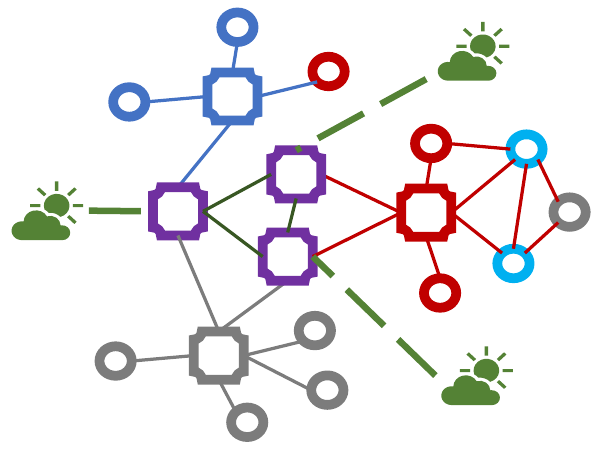
\includegraphics{images/questions/Schermata del 2023-10-19 10-03-17.png}
   % \caption{}
   \label{fig:dom1}
\end{figure}
Un problema comune nelle reti di device IoT sono i \textit{Vertical Silos}, business model adottato da diversi vendor, che porta le soluzioni IoT ad avere vari \textbf{vendor lock-in}, fra cui la limitatezza dei protocolli utilizzabili dai dispositivi prodotti.\\
Il problema è parzialmente risolto dagli \textbf{standard} di comunicazione, che tuttavia possono comunque essere ``troppi'' in una rete ampia, creando la necessità di tradurre da uno all'altro per permettere l'interoperabilità fra dispositivi di vendor diversi.\\
Primo argine al problema sono i \textbf{service gateway} (azzurro, rosso e grigio in figura), che permettono agli end-device di comunicare con internet (o altri gateway come in figura) e ad internet di comunicare con essi attraverso un endpoint unificato.\\
\ul{I dispositivi sono partizionati} \textit{non} in base al vendor, bensì \ul{al protocollo di comunicazione} che utilizzano.

Quella rappresentata in figura è una rete formata da \textbf{integration gateway} distribuiti che eseguono un mapping dai protocolli usati da end-device e service gateway (``non-viola'' in figura) a un linguaggio intermedio utilizzato per le comunicazioni fra di essi, e poi nuovamente mappato in un altro protocollo.
Questo permette di avere $2n$ mapping piuttosto che $n\times n$.
\note{Nella figura sembra che utilizzino lo stesso protocollo ``verde'' per comunicare con internet, ma non è necessario.}

All'interno di reti composte da device appartenenti a vendor (costruttori) diversi, che utilizzano protocolli diversi, è necessario l'utilizzo di un integration gateway per permettere l'interoperabilità tra i vari device.
%L'integration gateway quando non ha la capacità di tradurre un protocollo, traduce il comportamento di un device che utilizza un determinato protocollo in modo tale che device appartenenti ad altri vendor possano interagire con esso.
Mentre tradurre la serializzazione di un oggetto può essere vista come una funzione bigettiva/invertibile, per, ad esempio, richieste e risposte la traduzione da e verso il protocollo intermedio può richiedere operazioni differenti, da cui la necessità di $2n$ mapping, $\textit{n protocolli} \longrightarrow {lang\;intermedio}$ e viceversa.

\section{Sicurezza nei sistemi IoT}

\begin{figure}[htbp]
   \centering
   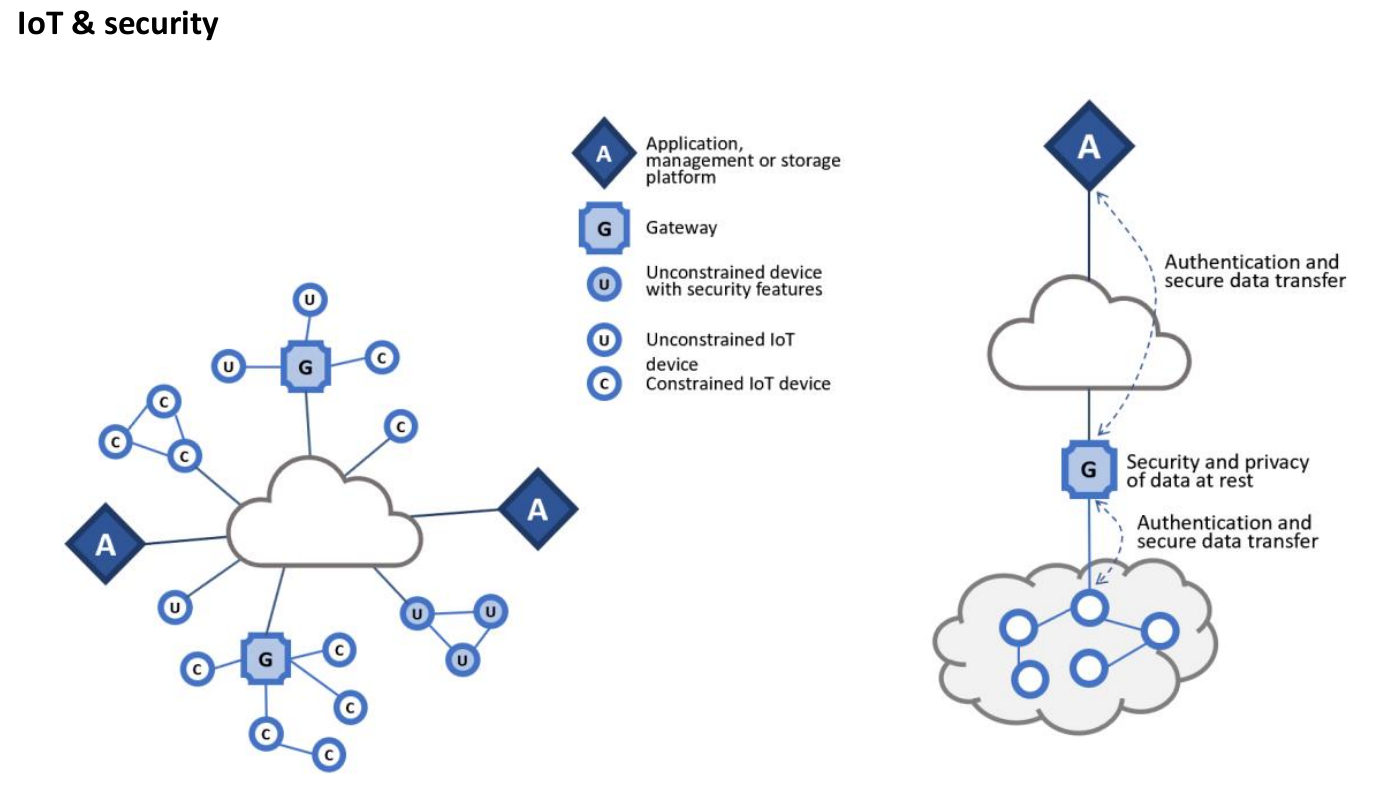
\includegraphics{images/questions/Schermata del 2023-10-16 18-20-38.png}
   % \caption{}
   \label{fig:dom2}
\end{figure}
Il tema della sicurezza in ambito IoT è un tema molto importante, in quanto per loro natura molte volte i dispositivi IoT sono sprovvisti di feature di sicurezza. Questo problema deriva dal fatto che i costruttori di questi device  danno priorità al time-to-market e al minimizzare il costo di produzione, a scapito della sicurezza:
le performance sono affette negativamente da essa, così come la durata della batteria. Spesso il sistema operativo installato è ``leggero'' e quindi privo di quelle funzionalità di security integrate all'interno di un sistema operativo full-fledged;
inoltre raramente vengono realizzate patch di sicurezza per i dispositivi IoT, e anche in tal caso è difficile applicarle. 

Per questo motivo sono stati standardizzati dall'ITU-T nel documento \texttt{Y.2066} dei \textit{requisiti di sicurezza} che riguardano diversi ambiti, tra i quali: comunicazioni, mutua autenticazione e autorizzazione, gestione dei dati, fornitura dei servizi, integrazione di politiche e tecniche di sicurezza e infine di security audit.
Tuttavia, non viene specificato come implementare soluzioni che soddisfino tali requirements.

Il focus dell'immagine è quello di mostrare quanto sia difficile garantire la sicurezza di una rete IoT, soprattutto in prossimità dei punti di accesso alla rete, questo dovuto anche al fatto che i dispositivi connessi sono di diversi tipi, esistono infatti dispositivi \emph{constrained} con limitate capacità computazionali e sprovvisti di ogni funzionalità di sicurezza, dispositivi \emph{uncostrained} con un'alta capacità computazionale ma senza funzionalità di sicurezza e altri dispositivi \emph{uncostrained} che però implementano funzionalità di sicurezza.\\
L'autenticazione mutua o one-way è fornita dai gateway. La sicurezza dei dati che si pone su tre livelli diversi: 

\begin{enumerate}
\item i dati salvati nei gateway e sui dispositivi;
\item i dati trasferiti tra gateway e dispositivi;
\item i dati trasferiti tra gateway e applicazioni.
\end{enumerate}

Tali requisiti di sicurezza diventano però difficili da soddisfare quando parliamo di constrained device, i quali raramente possono gestire encryption e autenticazione, portando a problemi di privacy sui dati, soprattutto riguardo i dispositivi nelle case.
È il caso dei dispositivi ``c'' in figura esposti direttamente a internet. 
\note{Possibile esempio climatizzazione, luci, frigo ecc\dots Oppure wristband e heart rate}

\section{Publish/subscribe e MQTT}

\begin{figure}[htbp]
   \centering
   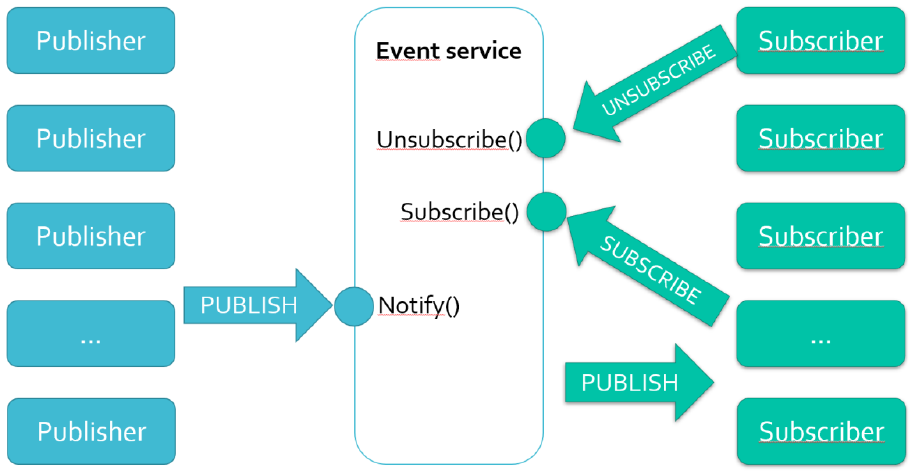
\includegraphics{images/questions/Schermata del 2023-10-19 12-23-59.png}
   % \caption{}
   \label{fig:dom3}
\end{figure}

MQTT è un protocollo di trasporto di messaggi affidabile e leggero basato sul modello publish/subscribe, un modello di comunicazione asincrona basato su eventi in cui sono coinvolte tre tipologie di entità: 

\begin{itemize}
\item il message broker, o event service: funziona come un server che gestisce lo scambio dei messaggi basato su topic;
\item i publisher: funzionano come client che pubblicano messaggi sul message broker marcandoli con un determinato topic;
\item i subscriber: funzionano come client e si sottoscrivono ad un determinato topic sul message broker.
\end{itemize}
\note{I client devono conoscere l'IP/hostname del broker \textit{beforehand}, essendo MQTT basato su TCP/IP.
I client sono identificati dal broker attraverso un \textit{Client ID} che deve essere univoco.}

Quando un publisher pubblica un nuovo messaggio su un topic il message broker invia una notifica a tutti i subscriber che sono iscritti a quel topic, se ne esistono. Ogni subscriber è libero di disiscriversi da un determinato topic in ogni momento.
\note{I subscriber potrebbero anche essere offline al momento del publish, ma comunque ricevere successivamente il messaggio (se e solo se i messaggi hanno QoS 1 e 2) in caso abbiano richiesto una sessione persistente;
i messaggi possono anche essere \textit{retained}, e in tal caso vengono inoltrati non appena un client si sottoscrive al topic di appartenenza.}

Questo modello permette la non dipendenza tra spazio, tempo e sincronizzazione facendo si che tutti gli agenti possano lavorare in modo indipendente senza dover attendere il lavoro di altri. La scalabilità è inoltre migliore rispetto a un generico client/server, in quanto basta aggiungere più broker che funzionano in paralleo.

Il broker può filtrare i messaggi basandosi su tipo, contenuto e \textit{topic}.

\section{MQTT esempio di interazione e QoS}

\begin{figure}[htbp]
   \centering
   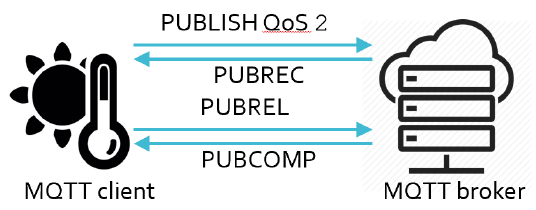
\includegraphics{images/questions/Schermata del 2023-10-19 15-29-05.png}
   % \caption{}
   \label{fig:dom4}
\end{figure}

Nell'immagine viene mostrato uno scambio di messaggi tra un client e il broker MQTT (event service) in cui nello specifico si nota il QoS 2 del pacchetto inviato. MQTT infatti offre una politica di QoS che risulta essere un accordo tra client e broker con 3 diversi livelli:

\begin{itemize}
\item Livello 0 (at most once): consegna best-effort senza garanzie, dove non abbiamo riscontri da parte del broker/server, il quale non salva i messaggi (neanche in caso di sessione persistente);
\item Livello 1 (at least once): consegna garantita almeno una volta al destinatario, dove il broker conferma la ricezione del messaggio tramite una risposta \texttt{PUBACK} (il messaggio può anche essere recapitato più volte);
il broker invia il messaggio ai subscriber subito. In caso \texttt{PUBACK} sia perso, il client invierà di nuovo il messaggio, e il broker potrà scartare il duplicato (non per forza), ma qualora avesse scartato il riferimento al messaggio (e.g. refresh cache), il messaggio duplicato verrà processato nuovamente e inviato ai subscriber.

\item Livello 2 (exactly once): garantisce la consegna esattamente una volta attraverso doppio two-way handshake, dove il broker notifica prima la ricezione del messaggio tramite un messaggio \texttt{PUBREC}, il client elimina il messaggio e risponde con \texttt{PUBREL} (\textit{``Release''}), il broker scarta il riferimento al messaggio e solo adesso lo invia ai subscriber, infine termina lo scambio con \texttt{PUBCOMP} (\textit{``Complete''}).
\end{itemize}

\note{Solo \texttt{PUBREC} non risulta essere sufficiente, dato che se perso, il client manderà di nuovo un messaggio, quindi il broker deve salvare un riferimento del messaggio, che verrà scartato quando otterrà \texttt{PUBREL}.}
\section{MQTT}

\begin{enumerate}
\item \textit{Explain how messages are filtered by the broker and what are the topics in MQTT:} I messaggi vengono filtrati dal broker basandosi su tre diverse caratteristiche: il topic del soggetto (cioè l'argomento di interesse che tipicamente è una stringa), il contenuto (cioè una specifica query che controlla uno o più dati) oppure sul tipo (cioè controllando sia il contenuto che la struttura riferendosi ad una classe/tipo di dati). 

I topic sono stringhe organizzate in una gerarchia (ognuna separata da "/") che permettono di identificare un argomento di interesse. 
I subscriber possono utilizzare le wildcards per specificare un gruppo di topics:
\begin{itemize}
   \item \texttt{home/firstfloor/\textred{+}/presence}\\
   Seleziona tutti i \texttt{presence} sensors in tutte le stanze di \texttt{firstfloor}.
   Il \textred{+} è una wildcard che seleziona un solo livello della gerarchia.
   \item \texttt{home/firstfloor/\textred{\#}}\\
   Seleziona tutti i sensori del primo piano.
   Il \textred{\#} è una wildcard che seleziona tutti i rimanenti livelli della gerarchia, deve essere l'ultimo carattere del topic.
   \item I topic che iniziano con il carattere ``\texttt{\textred{\$}}'' sono riservati per statistiche interne di MQTT;
   Questi topic non sono standardizzati, e non possono essere pubblicati dai client.
\end{itemize}

\note{Notare che isciversi a \texttt{/home/firstfloor}, \textbf{non} significa ricevere notifiche per i messaggi relativi a tutti i subtopic come \texttt{/home/firstfloor/presence}, è necessario usare l'opportuna wildcard multilivello \textred{\#}}


\item \textit{Explain the persistent sessions in MQTT:} Una sessione persistente mantiene lo stato tra il client e il broker, e.g. se un subscriber si disconnette, quando si connette nuovamente non ha bisogno di iscriversi ancora una volta ai topic a cui era sottoscritto. Le sessioni sono associate al \emph{clientId}. 
È necessario richiedere la sessione persistente al momento della connessione, settando a \texttt{FALSE} il flag \texttt{Clean Session}.\\
Il broker memorizza tutte le iscrizioni, tutti i messaggi con QoS 1 e 2 non ancora confermati e che arrivano quando il client è offline.
\note{Si ricorda che il \texttt{Client ID} deve essere univoco per evitare complicazioni.}

\item \textit{Explain the retained messages in MQTT}: I retained message sono messaggi utilizzati dai publisher che vogliono tenere aggiornati i nuovi subscriber sullo stato delle comunicazioni. Questi messaggi sono semplici messaggi con il \emph{retainFlag} settato a \textbf{true}, ciò permette al broker di salvare e poi recapitare il messaggio ad un nuovo client che si sottoscrive a quel determinato topic, anche se il messaggio ha QoS 0. Solitamente questa tipologia di messaggi viene utilizzata per aggiornamenti non frequenti dello stato, come ad esempio lo stato di apertura/chiusura di una porta.


\item \textit{Explain the Lastwill\&testament and the Keep Alive mechanism in MQTT:} Sono due meccanismi utilizzati in MQTT, e fanno riferimento agli omonimi campi nel messaggio \texttt{CONNECT}:
\begin{enumerate}
   \item \textbf{LastWill\&Testament} è una feature che viene impostata a tempo di connessione da un client per notificare gli altri client in caso di una sua disconnessione improvvisa. Quando il broker riscontrerà una disconnessione improvvisa del client invierà il messaggio indicato a tutti gli iscritti del topic specificato quando la feature è stata impostata.

   \item \textbf{KeepAlive}: assicura che un client rimanga attivo, per farlo il client invia periodicamente un messaggio \texttt{PINGREQ} (seguito da \texttt{PINGRESP}) al broker prima che l'intervallo definito nel campo. Se questo non avviene in tempo il broker termina la connessione ed invia il messaggio \textit{LastWill\&Testament} se presente.
\end{enumerate}
\end{enumerate}

\newpage
\section{Zigbee I}

\begin{figure}[htbp]
   \centering
   \includegraphics{images/questions/Schermata del 2023-10-19 15-30-53.png}
   % \caption{}
   \label{fig:dom6}
\end{figure}

Un device ZigBee può connettersi a una PAN in seguito a una richiesta specifica del Coordinator: in tal caso si tratta di \textbf{Direct Join}.
La figura invece illustra la procedura di \textbf{join through association} avviata da device ZigBee con un Coordinator di una PAN selezionata a seguito di una scansione preliminare.\\ 
I messaggi in sequenza sono:

\begin{enumerate}
\item La prima richiesta inviata è una \texttt{NETWORK-DISCOVERY.request}, che il livello applicativo manda al sottostante livello di rete per identificare le PAN disponibili;
\item Il livello di rete inoltra tale richiesta al livello MAC ---inviando una \texttt{SCAN.request}--- che avvia una active scan che restituisce al livello di rete una serie di PAN ID, con informazioni sui relativi router/coordinator, attraverso una \texttt{SCAN.confirm};
\item Il livello di rete propaga a livello applicazione il set di PAN ID con \texttt{NETWORK-DISCOVERY.confirm}, permettendo la selezione della PAN a cui unirsi;
\item La \texttt{JOIN.request}, che viene inoltrata al network layer, contiene dei parametri come \ul{l'identificatore della PAN scelta}, un flag che indica il tipo di dispositivo che si unisce (router o end-device);
\item A livello rete viene selezionato il nodo ``genitore'' corrispondente alla PAN scelta;
\item Questo porta poi all'invio di \texttt{ASSOCIATE.request} verso il livello MAC che avvia il protocollo di associazione in cui si ottiene l'indirizzo breve a 16-bit.
\item L'indirizzo di livello rete NWK lungo 16 bit (e.g. \texttt{0x0FF3})\footnote{Max address is \texttt{0xFFFF}} viene restituito a livello rete da \texttt{ASSOCIATE.confirm} e poi propagato a livello applicazione da \texttt{JOIN.confirm}.
\end{enumerate}

\section{Zigbee II}
\begin{figure}[htbp]
   \centering
   \includegraphics{images/questions/Schermata del 2023-10-19 15-32-10.png}
   % \caption{}
   \label{fig:dom7}
\end{figure}
   
Nella figura viene rappresentato il livello applicazione di ZigBee a sua volta diviso in 3 sotto-livelli:

\begin{itemize}
\item \textbf{Application Framework}: contiene fino a 240 \emph{Application Object (APO)}, ovvero applicazioni ZigBee definite e implementate dall'utente. Ogni APO è identificato in modo univoco all'interno della rete e i più semplici possono essere interrogati utilizzando il \emph{Key Value Pair (KVP) data service}.
Gli APO più complessi al contrario, possono gestire al loro interno anche uno stato più complicato; di conseguenza necessitano l'interazione con il \emph{Message data service}. Ciascun APO rappresenta un componente singolo del device (e.g., lampadina di un dispositivo o interruttore);
\item \textbf{ZigBee Device Object (ZDO)}: è un'applicazione speciale situata sull'endpoint 0 e gestisce il comportamento di un device in una rete ZigBee. 
\note{Dunque implementa le funzionalità di end-device, router o coordinator. Implementa comportamenti come rispondere a una device discovery.}
Un profilo speciale, lo \textit{ZigBee Device Profile}, descrive i cluster che devono essere supportati da ogni device ZigBee, che sono implementati dallo ZDO.
In particolare sono implementati i servizi di (device e service) discovery e binding, e come gestisce network e sicurezza. 
\begin{itemize}
   \item device e service discovery;
   
   \item binding management;
   
   \item network management;
   
   \item node management
\end{itemize}
\item \textbf{Application Support Sublayer (APS)}: è una sorta di livello di trasporto, simile a TCP, ma offre funzionalità diverse. È responsabile principalmente di fornire dati e gestire i servizi agli APO e ZDO. Inoltre, definisce:
\begin{itemize}
   \item gli endpoint: identificatori univoci degli APO che vanno da 1 a 240;
   
   \item i cluster: protocolli che definiscono un set di messaggi e comandi che i device possono usare per comunicare, ogni cluster è identificato in modo univoco tramite un cluster ID;
   
   \item profile ID e device ID.
\end{itemize}

Uno dei servizi fondamentali dell'APS è l'APS binding che permette di interconnettere l'endpoint di un nodo con uno o più endpoint di un altro nodo. Inoltre, il binding è unidirezionale e può essere gestito dallo ZDO di un coordinatore o di un router. \\
Nell'APS risiedono l'\textbf{Address Map} e la \textbf{Binding Table}.
\end{itemize}

Il \textbf{Network Layer} fornisce gestisce l'addressing, il routing e funzionalità di sicurezza (No SSL, si utilizza AES-128 o nell'APS o nel NWK); infatti gli indirizzi NWK servono per l'identificazione dei device (e APOs).
Fornisce un livello di astrazione rispetto al \textbf{MAC layer}, che opera più a basso livello astraendo dal livello fisico e occupandosi di (ri)trasmissione/ricezione dei frame, scan delle reti disponibili, unione a una rete, ecc.

\section{Topologie ZigBee}

\begin{figure}[htbp]
   \centering
   \includegraphics{images/questions/Schermata del 2023-10-19 15-34-16.png}
   % \caption{}
   \label{fig:dom8}
\end{figure}

Possiamo distinguere tre tipo di topologie di rete:

\begin{itemize}
\item \textbf{Topologia a stella}: il nodo centrale è sempre un coordinatore, mentre gli altri nodi possono essere indifferentemente router o end-device che svolgono lo stesso ruolo. Per la comunicazione utilizzano il \emph{superframe};
\item \textbf{Topologia ad albero}: sfrutta i router per ampliare la copertura della rete. Il nodo radice sarà sempre un network coordinator, i router possono assumere il ruolo di nodi intermedi attraverso i quali avvengono le comunicazioni oppure possono essere nodi foglia, mentre gli end-device possono soltanto essere nodi foglia. Inoltre, vengono supportate le funzionalità della rete multi-hop;
\note{Superframe facoltativo}
\item \textbf{Topologia mesh}: Essenzialmente è una rete p2p multi-hop, con path multipli che portano alla stessa destinazione.
Anche se possibile utilizzarlo, la comunicazione è possibile anche tra nodi anche senza affidarsi all'infrastruttura superframe, sfruttando channel sharing e meccanismi di collision avoidance.
\end{itemize}

\section{ZigBee Address Tree}

\begin{figure}[htbp]
   \centering
   \includegraphics{images/questions/Schermata del 2023-10-19 15-35-42.png}
   % \caption{}
   \label{fig:dom9}
\end{figure}

Topologia basata su alberi viene sfruttata dal livello rete di ZigBee per assegnare l'indirizzo di rete breve basato su una politica definita dal coordinatore ZigBee. I parametri utilizzati sono:

\begin{itemize}
\item Il \textbf{massimo numero di router} che ogni router ha come figlio: \textbf{\emph{Rm}};
\item Il \textbf{massimo numero di dispositivi terminali} che ogni router ha come figlio: \textbf{\emph{Dm}};
\item La \textbf{massima lunghezza dell'albero}: \textbf{\emph{Lm}}.
\end{itemize}

Guardando l'immagine si ha una rete ad albero con \emph{Rm}=2, \emph{Dm}=2 e \emph{Lm}=3. Il coordinatore ha indice 0 e il suo figlio sinistro 1. Il numero massimo di nodi in questo esempio è 28 perché è la soglia data dai tre parametri prima descritti. Questo limita il numero di nuovi dispositivi che possono unirsi alla rete, quindi un nuovo dispositivo non può entrare nella rete se viene raggiunto il limite. L'assegnazione del range viene dato seguendo un ordine DFS.

Se il nodo 3 vuole comunicare con il nodo 25, deve inviare il pacchetto al nodo 2, ed essendo 25 fuori dal suo range esso deve mandare il pacchetto al nodo 1 (nodo padre) e per lo stesso motivo al nodo 0. Il pacchetto viene poi inviato al nodo 14 che ha nel suo range 25. Queste comunicazioni avvengono per maggioranza tra router, tranne tre, quella che porta da 14 a 25 poiché è un dispositivo terminale, ma anche quelle da 1 a 0 e da 0 a 14, visto che 0 è la root ed è un network coordinator.

\section{Tabella di binding ZigBee}

\begin{figure}[htbp]
   \centering
   \includegraphics{images/questions/Schermata del 2023-10-19 15-37-17.png}
   % \caption{}
   \label{fig:dom10}
\end{figure}

Tabella di binding gestita dal Application Support Sublayer (APS). L'operazione di binding permette ad un end-point (APO) di un device di connettersi ad uno o più end-point su altri nodi senza conoscerne il NWK address né tantomeno l'endpoint di destinazione: il binding è unidirezionale e può essere configurato solo dal ZDO del coordinator o di un router. \\
Il binding quindi fornisce un modo di non specificare l'indirizzo di destinazione di un messaggio (\textbf{Indirect Addressing}), opposto al più canonico metodo del \textbf{direct addressing} che prevede che la sorgente indichi la tupla $\langle$\texttt{destination address}, \texttt{destination endpoint}$\rangle$ e che potrebbe essere non applicabile per dispositivi molto semplici.
In questo modo, l'invio dei messaggi presso i destinatari è totalmente delegato a router e coordinator, dove risiede la binding table, tipicamente inizializzata a tempo di configurazione della rete, e aggiornata solo su esplicita richiesta dello ZDO di coordinator e router.



Le due primitive principali utilizzate per il binding sono BIND e UNBIND che servono rispettivamente per creare una nuova entry nella tabella di binding locale e per eliminarla. \\
La entry mantiene l'indirizzo sorgente (MAC a 64 bit), l'endpoint sorgente, l'identificatore del cluster, l'indirizzo a 64 bit di destinazione (o indirizzo 16 bit multicast\footnote{NON il NWK address a 16bit!!!}) e l'endpoint di destinazione. Questa tabella viene salvata in modo persistente nell'APS del coordinatore di ZigBee e/o di un altro router: viene caricata su esplicita richiesta del ZDO.

Un messaggio viene inoltrato alla/e destinazione/i trovando le entry che nella binding table matchano la tupla $\langle$\texttt{source address}, \texttt{source endpoint}, \texttt{clusterID}$\rangle$ del messaggio in arrivo. 
In caso di multipli match, avverrà una comunicazione multicast e il messaggio sarà inoltrato alle multiple destinazioni.
\note{In figura per la tupla $\langle 0x3232...,5,0x0006 \rangle$ abbiamo più entry corrispondenti a più destinazioni.}
\note{Se non ci sono match, il messaggio viene scartato.}

\section{Diagramma di configurazione e interconnessione delle luci}

\begin{figure}[htbp]
   \centering
   \includegraphics{images/questions/Schermata del 2023-10-19 15-41-05.png}
   % \caption{}
   \label{fig:dom11}
\end{figure}

Esempio di utilizzo della ZigBee Cluster Library (ZCL) che contiene le specifiche e i framework per i cluster implementati dalle applicazioni degli utenti. \ul{Per cluster si intende collezione di comandi e attributi relativi a un \textit{dominio funzionale}} (che definiscono un'interfaccia di una specifica funzionalità).
Tali comandi sono definiti seguendo un modello client-server, dove il dispositivo che salva gli attributi mantenendo uno stato interno è un server mentre i dispositivi che manipolano gli attributi sono client.\\
{\ns La ZCL definisce anche dei messaggi per:
\begin{itemize}
   \item Leggere/scrivere attributi
   \item Configurare un report e leggere una risposta in formato report
   \item Scoprire ID e tipi degli attributi supportati da un server 
\end{itemize}}

Nella figura si parla di cluster nel dominio funzionale \emph{Lighting} in cui si vuole configurare un insieme di APO con uno switch ON/OFF connesso con una ``simple lamp" e un ``dimmer switch" connesso ad una ``dimmable lamp", che sono i cluster. Il configuration tool crea l'associazione tra i due APO funzionando come un client che imposta la configurazione del dispositivo di switch in modo che quando la lampada sia accesa o spenta questo possa essere visto nel dispositivo corrispondente. Il configuration tool imposta una tabella di routing nel coordinator conoscendo l'indirizzo dei dispositivi e dei relativi APO.

\section{Duty Cycle I}

\begin{figure}[htbp]
   \centering
   \includegraphics{images/questions/Schermata del 2023-10-19 15-42-33.png}
   % \caption{}
   \label{fig:dom12}
\end{figure}

Il codice in figura mostra un esempio di un programma Arduino, in cui ogni componente viene accesso, utilizzato e poi successivamente subito spento per cercare di ottimizzare il consumo energetico del device su cui questo codice è installato. 
% Infatti il problema del consumo energetico è un problema centrale in ambito IoT, in quanto tali dispositivi hanno un ciclo di vita finito, dopo il quale devono essere sostituiti.
Per aumentare il lifetime è necessario ottimizzare il duty cycle di ogni componente, ovvero il rapporto tra il \ul{tempo di attività e e il periodo}\footnote{valore arbitrario maggiore o uguale del tempo di attività, onde evitare complicazioni nei calcoli}.
Il duty cycle complessivo di un dispositivo è pari alla somma dei duty cycle di ogni singolo componente, assumendo che i cicli di operatività siano ``disgiunti'' e alcune semplificazioni sull'effettivo istante di ON/OFF.
Ad esempio, \textit{Duty cycle = 1\%} implica che il device sia accesso solo per il 1\% del tempo totale, e spento per il restante 99\%.

Negli esercizi si considera il tempo richiesto per ciascuna operazione di CPU/Radio/Sensore/ecc. (in figura non riportato), e si rapporta al periodo complessivo (in figura il periodo \textbf{non} è 380!).

Per calcolare i consumi energetici, si fa riferimento alla tabella dei consumi tipicamente fornita per ogni dispositivo IoT. Data la capacità della batteria equipaggiata, è possibile calcolare l'expected lifetime, moltiplicando il duty cycle per il la corrente consumata di ciascun componente, sommando i risultati, e dividendo la capacità della batteria per tale numero.

\note{
   Duty cycle CPU = $1\% = 0.01$\\
   $0.01\cdot 8mA + 0.99\cdot 0.015mA = 0.095mA$\\
   $2000mAh / 0.095mA = 21052 ore = 2.4 anni$}


\section{Duty Cycle II}

\begin{figure}[htbp]
   \centering
   \includegraphics{images/questions/Schermata del 2023-10-19 15-44-53.png}
   % \caption{}
   \label{fig:dom13}
\end{figure}

{\ns In questo diagramma si ha il confronto tra due modelli con duty cycle differenti:
\begin{itemize}
\item Il primo modello ha un DC pari al 100\%, ovvero con ogni componente del device sempre in funzione;
\item Il secondo modello ha un DC pari al 5\%, ovvero con un tempo di inattività delle sue componenti pari al 95\%.
\end{itemize}}

Come è possibile osservare dal grafico, il secondo modello ha un tempo di vita della batteria maggiore rispetto al primo a parità di capacità della batteria, questo perché il tempo di utilizzo limitato incrementa sicuramente il tempo di vita di un sensore, ma d'altro canto richiede che le attività delle varie componenti del device siano schedulate in modo efficiente, per rispettare le performance attese.

È necessario fare il tuning dei parametri del duty cycle affinché non solo il dispositivo funzioni efficientemente, ma che tale duty cycle gli permetta di fare sampling in modo produttivo e di funzionare correttamente. (e.g. Un sensore della temperatura per una stanza in una casa, non può fare sampling ogni due giorni)
 
\section{Embedded programming I}

\begin{figure}[htbp]
   \centering
   \includegraphics{images/questions/Schermata del 2023-10-19 15-45-55.png}
   % \caption{}
   \label{fig:dom14}
\end{figure}

Arduino è single threaded e il suo flow di esecuzione è una singola loop function che può invocare altre funzioni.
Non c'è la sospensione del thread, dunque operazioni di I/O fanno attendere il main thread finché non sono completate.
Gli step dell'esecuzione sono i seguenti:

\begin{enumerate}
\item Il device invoca la funzione \texttt{init} che permette l'inizializzazione del dispositivo stesso e abilita la comunicazione con i componenti hardware;
\item Viene invocato il main \texttt{loop()} rappresentante il ciclo delle operazioni da svolgere periodicamente.
\item Nell'esempio viene inviato un comando a una componente hardware; quando è stato eseguito l'Arduino RTS invia un segnale di terminazione del comando e restituisce il controllo al main loop;
\item Se il carico di lavoro attivo è stato compiuto si può invocare in modo esplicito la funzione \texttt{delay} che invia un comando ad un timer sospendendo la CPU finché il timer riattiva il \texttt{main loop} con un segnale (\texttt{timer fires}).
\end{enumerate}

\section{Embedded programming II}

\begin{figure}[htbp]
   \centering
   \includegraphics{images/questions/Schermata del 2023-10-19 15-47-07.png}
   % \caption{}
   \label{fig:dom15}
\end{figure}

In figura viene mostrato come TinyOS gestisce il software di un device, progettato per gestire principalmente eventi asincroni attraverso 3 concetti fondamentali:

\begin{itemize}
\item \textit{Comandi}: utilizzati per programmare e comunicare con l'hardware.
\item \textit{Eventi}: astraggono interruzioni hardware come una sorta di upcall.
\item \textit{Task}: definiti per gestire attività differenti e indipendenti. Quando un task è terminato e non ce ne sono altri da eseguire allora la CPU passa in \texttt{idle mode};
\end{itemize}

\begin{enumerate}
   \item La funzione \texttt{init} dopo aver inizializzato il device setta un timer e un handler da eseguire allo scadere.
   \item \texttt{timer handler} ---definita dall'utente oppure fornita dal RTS--- può, ad esempio, richiedere una lettura da un sensore; 
   \item Terminata la lettura, un \texttt{read handler} gestirà questo evento schedulando un nuovo task (ad alto livello) che potrà eseguire operazioni più complesse sui dati.
   \item Terminate le operazioni sui dati, questi saranno inviati all'hardware e verrà settato nuovamente un timer, che farà ripartire il ciclo degli eventi come successivamente alla funzione di init.
   \item TinyOS gestisce l'esecuzione di un singolo handler alla volta alla volta e infatti dovrebbero essere brevi: più interruzioni simultanee potrebbero causare seri problemi di concorrenza.Tuttavia è possibile che un'operazione hardware in corso (come l'ultima lettura in figura) possa essere interrotta da un'altra ``upcall''.
\end{enumerate}
I comandi invocati dagli handler non devono riguardare il componente HW che ha triggerato l'handler, onde evitare stati inconsistenti.

Con questo modello una task ``non aspetta mai'' che venga eseguita lettura o scrittura hardware, e può essere pre-empted solo da degli eventi; non sarà lei a richiedere esplicitamente di andare in idle, come nel caso di Arduino con il comando \texttt{delay}.

\section{Interruzioni Arduino}

\begin{figure}[htbp]
   \centering
   \includegraphics{images/questions/Schermata del 2023-10-20 11-32-10.png}
   % \caption{}
   \label{fig:dom16}
\end{figure}

Nel codice si può osservare il meccanismo delle interruzioni di Arduino che, come in TinyOS, permette di gestire eventi asincroni. Le interruzioni possono essere di tre tipi: \textit{esterne}, \textit{timer} o di \textit{dispositivo}. 
Esse vengono gestite dal RTS. In questo caso osserviamo come si ha una funzione di \lstinline{loop} principale in cui c'è un'attesa fissa che viene seguita da una scrittura digitale. All'occorrenza di un'interruzione \textit{esterna} è possibile come in questo caso definire un comportamento predefinito attraverso la funzione \lstinline{attachInterrupt(interrupt\#, funct-name, mode)} nella funzione di \lstinline{setup()}. Le modalità sono le seguenti:

\begin{itemize}
\item \textbf{RISING}: l'interruzione avviene quando il pin passa da un valore LOW ad un valore HIGH;
\item \textbf{FALLING}: l'interruzione avviene quando il pin passa da un valore HIGH ad un valore LOW;
\item \textbf{CHANGE}: l'interruzione avviene quando il pin cambia stato;
\item \textbf{LOW}: l'interruzione avviene quando il pin ha uno stato basso. Non necessariamente un cambio di stato, se rimane LOW l'interruzione avviene di nuovo;
\item \textbf{HIGH}: l'interruzione avviene quando il pin ha uno stato alto. Non necessariamente un cambio di stato, se rimane HIGH l'interruzione avviene di nuovo.
\end{itemize}

Nella figura, \lstinline{greenlLed = 7} definisce il pin 7 come il pin di output per il led verde, mentre \lstinline{attachInterrupt(0, interruptSwitchGreen, CHANGE)} definisce che l'interruzione avverrà sul pin 2 (corrispondente all'interruzione 0) e che la funzione \lstinline{interruptSwitchGreen} verrà eseguita quando il pin passerà da \lstinline{LOW} ad \lstinline{HIGH} (il cambio di stato è \lstinline{RISING}). \lstinline{interruptSwitchGreen} è una funzione che cambia lo stato del led verde.
\lstinline{Serial.begin(9600)} setta il data rate di trasmissione a 9600bit/s

\note{Saper spiegare il resto del codice a voce}

\section{SMAC}

\begin{figure}[htbp]
   \centering
   \includegraphics{images/questions/Schermata del 2023-10-20 11-35-40.png}
   % \caption{}
   \label{fig:dom17}
\end{figure}

Lo schema in figura rappresenta lo scambio di messaggi tramite l'utilizzo del protocollo SMAC, un protocollo MAC (\textit{Medium Access Control}) per le reti wireless multihop.
SMAC è utilizzato in 802.11, mentre in 802.15.4 si utilizza il \textbf{polling} (beacon).
In questo protocollo i nodi utilizzano una sincronizzazione locale per poter comunicare con i propri vicini, ottenuta tramite lo \ul{scambio di messaggi \texttt{SYNC} che permettono di sincronizzare i duty cycle} ---della radio--- dei dispositivi in modo che si accendano nello stesso momento.

Qualora un nodo voglia inviare a un ricevente che non è sincronizzato con il suo stesso ciclo, dovrà comunicare nel time slot del nodo ricevente, eventualmente svegliandosi fuori dal suo slot predefinito.

Visto che le comunicazioni avvengono nel timeframe del ricevente è possibile che si vengano a creare delle collisioni, per questo motivo prima di inviare un messaggio viene effettuato un controllo \textit{Carrier Sense} per comprendere se il canale sia occupato o meno, causando ritardi nella trasmissione. Se vengono ricevuti o un \texttt{RTS} (Request To Send) o un \texttt{CTS} (Clear To Send) la trasmissione viene lasciata attiva perché questa sia terminata.

Questo protocollo ha due problemi principali, il primo, la \textbf{latenza}, dovuta alla difficoltà nel sincronizzare molteplici nodi distanti (resa accettabile da cluster di nodi vicini che invece riescono a sincronizzarsi), mentre il secondo è la qualità degli \textbf{orologi interni} dei device (spesso cheap), che possono portare a oscillazioni nella misurazione del tempo e dunque a desincronizzazioni.

\note{Inoltre il CSMA/CA usato ha i problemi di \textit{hidden/exposed terminal}.}

\section{BMAC}

\begin{figure}[htbp]
   \centering
   \includegraphics{images/questions/Schermata del 2023-10-20 11-36-52.png}
   % \caption{}
   \label{fig:dom18}
\end{figure}

Lo schema in figura rappresenta lo scambio di dati attraverso il protocollo BMAC. Il protocollo BMAC è un protocollo \emph{medium access control} che riduce la complessità del protocollo SMAC, in quanto richiede la configurazione di un unico parametro, stabilito out-of-band.

In questo protocollo il mittente può inviare un messaggio che contiene un lungo preambolo (preamble), in qualsiasi momento. Al contrario il ricevente attiva la radio periodicamente controllando se c'è un preamble che deve essere catturato (preamble sampling) basandosi sulla modalità \emph{Low-Power Listening (LPL)}.\\
Questi preamble dovranno avere una lunghezza maggiore rispetto all'intervallo che avviene tra un campionamento ed un altro e un punto a sfavore risiede nel fatto che il ricevente deve attendere la fine del preamble prima di ricevere i dati.
\note{Viene da chiedersi se un nodo prima di inviare un preambolo debba provare ad ascoltare per  capire se il canale non sia già occupato, o se invece sia legato al spike rosso indicante il wake-up}

Il protocollo permette ai receiver di utilizzare meno energia, a scapito dei consumi maggiori del sender; dunque BMAC trova un'utile applicazione in scenari dove ci sono più receiver e pochi sender.

\section{Device Lifetime e BMAC}

\begin{figure}[htbp]
   \centering
   \includegraphics{images/questions/Schermata del 2023-10-20 11-37-09.png}
   % \caption{}
   \label{fig:dom19}
\end{figure}

Il diagramma in figura mostra l'andamento del tempo di vita di un \textbf{trasmettitore} mettendo in rapporto la frequenza di invio dei sample, il tempo fra i wake-up ($t_check$), e gli anni di vita di un dispositivo. Si può osservare come ad una frequenza di campionamento maggiore (per esempio 1 sample al minuto - linea rossa) il tempo di vita sia molto breve, addirittura inferiore ai 3 anni, mentre con un campionamento meno frequente (per esempio 1 sample ogni 20 minuti - linea verde), il tempo di vita aumenta sensibilmente raggiungendo un massimo che supera sfiora 3 volte il tempo di vita usando il campionamento con la linea rossa.

%The node lifetime depends on the check interval (of preamble sampling) and the total amount of traffic in the network cell.
Ciò che è interessante è vedere come indipendentemente dalla frequenza dei sample, il trend sia comunque decrescente oltre un certo $t_{check}$, il tempo fra un risveglio e l'altro, indicante anche la lunghezza del preambolo da mandare.


\note{
Tali valori sono ottenuti attraverso le seguenti formule che formalizzano il tempo di vita di un trasmettitore:

\begin{itemize}
\item $DC_{tx}=f_{data}\cdot(t_{preamble}+t_{data})$

\item dove abbiamo $f_{data}$ frequenza di invio dei dati, $t_{preamble}$ l'intervallo di invio del preamble, $t_{data}$ l'intervallo di invio dei dati.
\item $DC_{check}=f_{check}\cdot t_{check}$

\item dove abbiamo $f_{check}$ la frequenza di sampling, $t_{check}$ l'intervallo di sample frequency
\item $ET(t)=t\cdot(p_{tx}DC_{tx}+p_{tx}DC_{check}+p_{sleep}*(1-DC_{tx}-DC_{check}))$


\item dove $p_{tx}, p_{sleep}$ rappresentano rispettivamente il consumo energetico durante la fase di trasmissione e il consumo energetico durante la fase di riposo
\end{itemize}
\textred{TODO verifica formule se sono scritte bene}
}


\section{XMAC/BMAC}

\begin{figure}[htbp]
   \centering
   \includegraphics{images/questions/Schermata del 2023-10-20 11-48-12.png}
   % \caption{}
   \label{fig:dom20}
\end{figure}

Il protocollo X-MAC è un'evoluzione del protocollo B-MAC che mira a ridurre l'impiego di lunghi preamble vuoti. 

Per fare ciò il protocollo permette al ricevente di fermare l'invio del preamble inviando un ACK:\\
quando un receiver trova il suo ID all'interno di uno dei preamble brevi inviati da un sender allora questo invierà un early ACK al sender che sospenderà l'invio dei preamble e invierà i dati al ricevente che è pronto a riceverli. 
\note{Il ricevente dopo la ricezione dei dati non spegnerà immediatamente la componente radio per permettere ad altri eventuali nodi di inviargli dati nel caso in cui abbiano trovato il canale precedentemente occupato.}

Nell'immagine si può vedere come in XMAC nella fase di trasmissione invia un preambolo breve contenente informazioni sull'indirizzo dei target, quando il ricevente si sveglia e cattura il preambolo breve replica con un ACK che permette al mittente di iniziare l'invio dei preamboli brevi e di iniziare ad inviare i frame con i dati.

BoX-MAC è un'ulteriore sviluppo di XMAC, in cui si sostituisce il preambolo con l'invio ripetuto dei dati (insieme alle informazioni sui destinatari).
\note{È adatto per applicazioni in cui i dati sono piccoli e la latenza è critica.}

\section{IEEE 802.15.4 superframe}

\begin{figure}[htbp]
   \centering
   \includegraphics{images/questions/Schermata del 2023-10-20 11-49-03.png}
   % \caption{}
   \label{fig:dom21}
\end{figure}

L'immagine mostra il servizio di channel access per il livello MAC del protocollo IEEE 802.04.15. Abbiamo due tipi di accesso a livello MAC:
{
   \ns
   \begin{enumerate}
      \item con superframe structure;
      \item senza superframe structure;
      \end{enumerate}
      
      }

Nello specifico l'immagine mostra un channel access con superframe structure, utilizzato solitamente nelle topologia a stella o nelle topologie peer-to-peer, ma con struttura ad albero.
In caso di reti \textit{non-beacon enable}, la comunicazione avviene senza superframe structure, con un protocollo unslotted \texttt{CSMA-CA};
il coordinator è sempre pronto a ricevere dati da un end-device mentre la trasmissione da end-device a coordinator è poll-based: l'end-device si sveglia periodicamente e interroga il coordinator per i messaggi in attesa.

Un superframe è composto da due parti, una attiva e l'altra inattiva. 
Tutte le comunicazioni avvengono durante il periodo attivo, mentre in quello inattivo i nodi possono andare in idle.  

La parte attiva, in cui è possibile comunicare è composta a sua volta da 15 time frame della stessa dimensione, di cui il primo di questi è detto beacon frame ed è inviato dal PAN coordinator. 
Il beacon frame serve per sincronizzare i dispositivi collegati, per identificare il PAN e descrivere la struttura del superframe. 

La comunicazione vera e propria tra l'end device e il coordinatore (\ul{non con i router}) avviene nella restante parte del periodi di attività, che è divisa in due parti:

\begin{itemize}
\item \textbf{Contention Access Period (CAP)}: il dispositivo compete per accedere al canale utilizzando il protocollo standard slotted CSMA/CA. 
Un dispositivo che vuole trasmettere i frame dati prima deve aspettare il beacon frame e dopo randomicamente seleziona uno slot temporale per la sua trasmissione: se seleziona uno slot occupato da un'altra comunicazione allora proverà a selezionarne un altro, altrimenti attenderà il successivo superframe.\\
Una volta iniziata la trasmissione, il sender tiene il canale occupato fino alla fine del frame.
\note{\ul{Il CAP period deve essere composto da almeno uno slot}, per permettere a nuovi device di unirsi alla rete}

\item \textbf{Contention Free Period (CFP)}: opzionale e utilizzato per applicazioni a bassa latenza o che richiedono uno specifico bandwidth. Il coordinatore PAN può assegnare porzioni di questa parte chiamati \textbf{GTS (Guaranteed Time Slot)} a specifiche applicazioni.
\note{In caso ci siano più richieste di GTS di quante ne siano disponibili, il coordinatore PAN può assegnare i GTS in base a priorità o in base a un algoritmo di scheduling, altrimenti risponde ai richiedenti ``picche'' \smiley.}
\end{itemize}

\section{Trasferimento dei dati IEEE 802.15.4}

\begin{figure}[htbp]
   \centering
   \includegraphics{images/questions/Schermata del 2023-10-20 11-49-16.png}
   % \caption{}
   \label{fig:dom22}
\end{figure}

Il sequence diagram nell'immagine mostra il trasferimento di dati da un \textit{coordinator} $\longrightarrow$ \textit{device} in una rete \textbf{beacon enabled}.
\\Esistono 3 diversi modelli di trasferimento dati: end-device al coordinatore, coordinatore all'end-device, peer-to-peer. 

\begin{itemize}
   \item coordinator a end device:\\
   il coordinator indica nel network beacon che esiste un messaggio per l'end device.\\
   Gli end device restano per la maggior parte del tempo in sleep mode, ma periodicamente si svegliano per controllare messaggi pending, e se ce ne sono li richiedono usando uno slot nel CAP.\\
   Il coordinator invia il pending message utilizzando anch'esso un protocollo CSMA-CA con slot all'interno del CAP. Una volta ricevuto il frame, il dispositivo può riconoscere la ricezione trasmettendo un ACK in uno slot temporale successivo;
   \item \note{end device a coordinator: il dispositivo attende il beacon di rete per sincronizzarsi con il superframe. Dopodiché, se possiede un GTS lo usa direttamente, altrimenti trasmette il data frame al coordinator utilizzando protocollo standard CSMA-CA in uno dei frame del CAP (Contention Access Period). Il coordinator riconosce la ricezione con successo trasmettendo un ACK in uno slot temporale successivo;}
\item \note{peer-to-peer: nel caso uno dei due dispositivi coinvolti nella comunicazione sia un end device allora si utilizza uno dei due protocolli sopra. Al contrario se entrambi i device sono coordinator e ognuno possiede il proprio network beacon, allora il mittente del messaggio deve sincronizzarsi prima con il network beacon del ricevente e comportarsi poi come un end device. }
\end{itemize}

\section{IEEE 802.15.4}

\begin{figure}[htbp]
   \centering
   \includegraphics{images/questions/Schermata del 2023-10-20 11-49-37.png}
   % \caption{}
   \label{fig:dom23}
\end{figure}

Il sequence diagram in figura rappresenta una richiesta di servizio ASSOCIATE, che viene invocato da un dispositivo che desidera associarsi con un PAN di cui ha l'identificativo da una invocazione preliminare del servizio SCAN. 

\begin{enumerate}
   \item La primitiva \texttt{ASSOCIATE.request} prende come parametro l'identificatore di una PAN, l'indirizzo del coordinatore e l'indirizzo IEEE esteso a 64 bit del dispositivo stesso.
   \note{La primitiva invia un messaggio di richiesta di associazione al coordinatore e, poiché la procedura di associazione è pensata per le reti abilitate al beacon, il messaggio di richiesta di associazione viene inviato durante il periodo CAP utilizzando il protocollo CSMA-CA.}
   \item 
   Il coordinatore invia un messaggio di ACK in cui riconosce la ricezione del messaggio ma non per questo l'associazione alla PAN è avvenuta con successo.
   \item Il coordinatore, attraverso la primitiva \texttt{ASSOCIATE.indication}, passa la richiesta al livello di rete dove viene effettuata la decisione sull'associazione:
   in caso questa sia accettata viene selezionato un indirizzo a 16 bit che il dispositivo utilizzerà in seguito al posto di quello IEEE da 64 bit.
   \item Il livello rete ritorna con la primitiva \texttt{ASSOCIATE.response} al livello MAC che prende come parametro l'indirizzo a 64 bit del dispositivo, il nuovo indirizzo a 16 bit e lo stato della richiesta.\\
   Il coordinatore genera così un pending message con la risposta dell'associazione.
   \item \ul{Dopo un periodo definito di attesa} il dispositivo fa una \textit{Data request} a cui corrisponde un ACK del coordinatore e a seguire il messaggio contenente la risposta dell'associazione, corrisposto da un ACK inviato dal device al coordinator
   \note{Deve essere il device a contattare il coordinator perché non conosce ancora il suo NWK address e il coordinator dovrebbe inserire tale address per inviargli un messaggio tramite il beacon.}
   \item Lato dispositivo quindi viene invocata la primitiva \texttt{ASSOCIATE.confirm} verso il livello rete mentre lato coordinatore viene emesso \texttt{COMM-STATUS.indication} per informare il livello superiore che il protocollo di associazione si è concluso (con successo o con un codice di errore).
\end{enumerate}

\section{Energy harvesting}

\subsection{Explain the difference between an harvest-use and an harvest-store-use architecture}

Nell'architettura \textbf{Harvest-Use} si ha un modello di harvesting diretto in cui non viene fornito nessun buffer energetico per questo l'energia accumulata viene immediatamente consumata. Questo comporta due principali svantaggi:
{\ns\begin{itemize}
   \item Spreco di energia quando quella prodotta è minore di quella consumata;   
   \item Spegnimento del dispositivo quando viene prodotta meno energia di quella consumata.
\end{itemize}}
Tale modello può funzionare in caso solo di fonti di energia ---molto--- prevedibili, o di carico di lavoro statico o facilmente adattabile.
   
      
Nel caso dell'architettura \textbf{Harvest-Store-Use} viene introdotto un buffer che permette la raccolta dell'energia in eccesso per usi futuri. 
Semplificazioni del modello potrebbero non tenere conto dell'efficienza di carica e degli energy leaks.
In base al materiale della batteria (\texttt{SLA}, \texttt{NiCD}, \texttt{NiMH}, \texttt{Li-on}, o supercapacitors) è possibile stimare alcuni dei comportamenti della batteria nel tempo.



\subsection{Explain the classification of sources in terms of controllability and predictability}
\begin{enumerate}
   \item \textbf{Controllabile} fornisce una raccolta di energia quando è richiesta
   \note{Self-powered flashlight, girando una manovella la luce si accende.}
   \item \textbf{Parzialmente controllabile} produce energia in modo limitato dall'ambiente %mentre le sorgenti di energia 
   \note{Sorgente di energa RF (energia a radiofrequenza) può fornire energia a RFID, ma non si possono controllare l'intensità di propagazione nella stanza (non possiamo garantire con precisione come questa si distribuirà nello spazio)}
   \item \textbf{Non controllabili} non possono essere attivate su richiesta
   \begin{enumerate}
      \item \textbf{prevedibili}: hanno dei modelli di utilizzo che ne descrivono la disponibilità
      \note{Sole}
      \item \textbf{imprevedibili}: indovina.
      \note{Terremoti}
   \end{enumerate}
\end{enumerate}
Le sorgenti più interessanti e maggiormente oggetto di studio sono quelle \textit{non} controllabili e prevedibili, in quanto permettono di avere un modello di harvesting più preciso e di conseguenza un modello di consumo più efficiente.

Il modello di Kansal tuttavia non richiede conoscenza sulla futura produzione di energia: le sorgenti devono essere ---anche solo in parte--- prevedibili, ma la stima di produzione energetica futura si basa esclusivamente sulle precedenti osservazioni;
Nonostante ciò il modello benificia da una maggior accuratezza in caso esistano dei modelli più avanzati di previsione.


\subsection{Explain the concept of energy neutrality}
Mentre il goal principale anni fa era di massimizzare la durata della batteria, oggi si cerca di ottenere la \textbf{neutralità energetica}: una produzione di energia che permette di ottenere lo stesso livello di performance per tutta la durata di un intervallo di tempo, i.e. la produzione e il consumo sono bilanciati e sostenibili nel tempo.

Kansal la formalizza stabilendo che $B(K+1) \geq B(1)$, ovvero la batteria al termine del periodo $K+1$ deve avere almeno la stessa carica di quella iniziale.


{Ci sono due aspetti chiave
\begin{itemize}
   \item \textbf{Energy-Neutral Operation}:\\
   Scegliere le operazioni da eseguire in modo che, in qualunque time frame, l'energia usata sia sempre inferiore di quella prodotta.
   \item \textbf{Maximum Performance}:\\
   Assicurando l'operatività energy-neutral (scritta sopra), determinare qual è il massimo livello di performance che si può ottenere in un dato ambiente di harvesting.
\end{itemize}
}

\section{Consumo di energia con buffer}

\begin{figure}[htbp]
   \centering
   \includegraphics{images/questions/Schermata del 2023-10-20 11-54-15.png}
   % \caption{}
   \label{fig:dom25}
\end{figure}

Rappresentazione grafica del modello \textbf{Harvest-Store-Use} in cui si hanno le due funzioni che rappresentano l'energia prodotta e quella consumata, e gli integrali rappresentano l'energia che viene immediatamente consumata appena prodotta (caso in cui $consumo > produzione$) oppure l'energia che viene immagazzinata (caso in cui $produzione > consumo$). In questo modello si considera un buffer ideale senza perdite e con capacità infinita.

Per ottenere l'energy neutrality dobbiamo garantire che l'area azzurra sia maggiore dell'area arancione, in modo da consentire di mantenere il dispositivo attivo anche quando l'energia prodotta è inferiore rispetto al consumo.\\
Inoltre dobbiamo anche massimizzare l'energia disponibile, per garantire le migliori performance possibili.

Per far ciò, Kansal formalizza il problema come un problema di ottimizzazione risolubile tramite la programmazione lineare, in cui si cerca di massimizzare l'utility del dispositivo, ovvero la somma delle utilità di tutte le operazioni eseguite\footnote{duty cycle per Kansal, task nel task-based model}, avendo come vincolo che il consumo di tali operazioni non ecceda l'energia disponibile.

\section{Esercizio harvesting}

\begin{figure}[htbp]
   \centering
   \includegraphics{images/questions/Schermata del 2023-10-20 11-56-49.png}
   % \caption{}
   \label{fig:dom26}
\end{figure}

$v_{max}$ indica la tensione fornita dalla batteria a piena carica ($B_{max}$), mentre $v_{min}$ corrisponde alla tensione fornita con la carica minima ($B_{min}$) che consente al dispositivo di funzionare.
Notare che tale carica minima, \textit{non} è una proprietà della batteria, bensì del sistema.

I dati rappresentati su $d$ bit $x_{min}$ e $x_{max}$ (e $x$ per un generico voltaggio $v$) che vengono letti dal ADC che ha in input il voltaggio, possono essere stimati matematicamente:
\begin{align}
    x_{max} &= 2^d -1\\
    x_{min} &= \left\lfloor\frac{v_{min}}{v_{max}}(2^d - 1)\right\rfloor\\
    x &= \left\lfloor\frac{v}{v_{max}}(2^d - 1)\right\rfloor
\end{align}

Il reference voltage $v_{ref}$ si calcola dividendo $v_{max}$ per il massimo intero rappresentabile con i bit dell'ADC ($2^d -1 = x_{max}$), e indica quanto ``pesa" un singolo bit.

Le ultime due colonne propongono un esempio di lettura di $x$ dall'ADC e calcolo del corrispondente livello di batteria, assumendo ---per comodità di calcolo--- che $B_{min} = 300mAh$, con la seguente formula:
\begin{align}
    B&= B_{min} + \frac{B_{max}-B_{min}}{x_{max} - x_{min}}(x-x_{min})
\end{align}
Tale formula assume una relazione lineare fra il voltaggio e la capacità della batteria, che è una approssimazione accettabile anche se in realtà dipende dalla batteria.
\begin{paracol}{2}
    \colfill
    Inoltre è opportuno osservare che il voltaggio della batteria decresce ``linearmente''(o progressivamente potrebbe rimanere circa costante) fino a una certa percentuale di carica, intorno al $10\%$, dopo il quale il voltaggio cala rapidamente verso 0, come in Fig. \ref{fig:discharge}.
    Tale punto dipende dalla batteria, nell'esempio si presume sia \texttt{300mAh}, circa un decimo della capacità totale.
    \colfill
    \switchcolumn
    \begin{figure}
        \centering
        \includegraphics{images/questions/discharge.png}
        \caption{Example of discharge graph of a Li-ion battery}
        \label{fig:discharge}
    \end{figure}
\end{paracol}

% \newpage
\section{Approccio di Kansal}

\begin{figure}[htbp]
   \centering
   \includegraphics{images/questions/Schermata del 2023-10-20 11-57-01.png}
   % \caption{}
   \label{fig:dom27}
\end{figure}

Il modello di Kansal per la neutralità energetica richiede delle assunzioni sulla fonte energetica, ovvero che sia non controllabile ma prevedibile, o quantomeno che l'\ul{energia da essa prodotta sia approssimabile ad una funzione lineare}.\\
Lo schema in figura è una rivisitazione di quello standard Harvest-Store-Use per implementare Kansal.\\
L'\textit{Energy predictor} realizza una stima della futura produzione di energia suddividendo il tempo in slot di dimensione fissa e usando l'EWMA come modello predittivo; infine comunica i risultati allo \textit{scheduler}.\\
Per ogni possibile duty cycle $dc$ si può calcolare un'utilità $u$ ---che va massimizzata--- e il consumo previsto $c$.
Lo scheduler, in base alle stime fornite dal predictor sull'energia e le informazioni $u$ e $c$ di ciascun $dc$, può assegnare ad ogni slot $dc$, massimizzando $u$ e garantendo la neutralità energetica.\\
Nella pratica questo può tradursi in duty cycle più o meno intensi a seconda dell'energia disponibile.

\subsection{Teorema di Kansal}
Il teorema stabilisce quali sono le condizioni sufficienti (non necessarie) per poter ottenere l'energy neutrality su un sistema.
\begin{align}
    \begin{cases}
        \eta \rho_s \geq \rho_c + \rho_{leak} \quad \text{Trend produzione maggiore di trend consumo e leak} \\
        B_0 \geq \eta \sigma + \delta \quad \text{$B_0$ sufficiente nel worst case} \\
        B_{max} \geq B_0 \quad \text{$B_0$ è un valore legale}
    \end{cases}
\end{align}
\note{Nella seconda equazione ---forse--- $\eta\sigma$ è un termine che starebbe a sinistra con segno negativo, ad indicare che invece di avere una produzione media (compresa fra $+\sigma$ e $-\sigma$) non si produce nulla. $\eta$ = coefficiente di efficienza di carica}

\framedt{Drawback}{
   Uno dei due principali drawback di questo modello è proprio che l'unico parametro che può essere variato per modificare il load è il \textbf{duty cycle}, rendendolo poco adattabile alla gestione di comportamenti più complessi.\\
   Inoltre in caso di sensori, alterare il duty cycle significa avere una misurazione con una \ul{frequenza di \textbf{campionamento} variabile}, che può rendere scomoda l'analisi dei dati.
   }


% Tale approccio prende in considerazione sia l'energia che la carica prevista della batteria, regolando dinamicamente le performance del dispositivo attraverso la regolazione del duty cycle e di conseguenza modificando il carico.

Il modello di Kansal assume che l'energia prodotta si possa approssimare ad una fonte lineare, ovvero che cresce limitata da due rette parallele che hanno un angolo pari a $\rho_s$. Da qui abbiamo che l'energia $E_T$ prodotta in un dato intervallo $[0, T]$ sia uguale a $E_T=\int_0^T P_S(T) dt$ e sia limitata come segue $\rho_s \cdot T-\alpha \leq E_T \leq \rho_s \cdot T+\alpha$ . 

Invece per quanto riguarda il carico (load), il modello di Kansal assume che sia limitato solo superiormente da una retta inclinata di un angolo $\rho_c$ e quindi abbiamo che il carico $L_T$ in un intervallo $[0,T]$ è uguale a $L_T=\int_0^T Pc(T)dt$ e quindi il carico sarà limitato nel seguente modo $0 \leq L_T \leq \rho_c \cdot T+\delta$


\note{
   Nel modello di Kansal il concetto di utility è legato al duty cycle nel seguente modo:
   \ns   
\begin{itemize}
\item $u(dc)=0 $ se $dc < dc_{min}$
\item $u(dc)=\alpha*dc+\beta$ se $dc_{min}\leq dc \leq dc_{max}$
\item $u(dc)=u_M$ se $dc > dc_{max}$
\end{itemize}

Con $u_M$ utility massima, $u_m$ utility minima, $dc_{max}$ duty cycle massimo, $dc_{min}$ duty cycle minimo e con
{\ns
\begin{align}
\alpha=\frac{u_{max}-u_{min}}{dc_{max}-dc_{min}}\\
\beta=u_{min}-\alpha*dc_{min}
\end{align}}
Dove in un grafico con assi $xy$ duty cycle $dc$ e utility $u$, $\alpha$ è il coefficiente lineare (\textit{inclinazione}) della retta, mentre $\beta$ è il punto in cui la retta incrocia l'asse y, ovvero l'\textit{offset} della retta.
}

\subsection{Modello di Kansal}
\begin{itemize}
   \item $k$ il numero di slot in un giorno
   \item $B(i)$ la carica della batteria all'inizio dello slot $i$
   \item $B(k+1)$ la carica della batteria alla fine del giorno
   \item $\tilde{p}_s(i)$ la stima della produzione di energia nello slot $i$
   \item[] \ul{Kansal assegna un $dc(i)$ (dunque una utility $u(i)$) a ciascuno slot $i$ in modo da massimizzare la somma delle utility di tutti gli slot, garantendo che $B(k+1) \geq B(1)$}, ovvero che la carica della batteria alla fine del giorno sia maggiore uguale a quella all'inizio del giorno.
\end{itemize}

\subsection{Algoritmo Kansal}
Si inizializzano gli slot assegnando $dc_{max}$ ai ``sun slot'' e $dc_{min}$ ai ``dark slot''.
A questo punto ---rispetto alla stima di produzione di energia $\tilde{p}_s(i)$--- si può riscontrare:
\begin{enumerate}
   \item \textbf{Overproduction}\\
   Si massimizza il $dc$ dei dark slot finché non si esaurisce l'energia sovrapprodotta
   \item \textbf{Underproduction}\\
   Si minimizza il $dc$ dei sun slot finché non si va in pari con l'energia prodotta
\end{enumerate}
\section{Modello basato su task}

\begin{figure}[htbp]
   \centering
   \includegraphics{images/questions/Schermata del 2023-10-20 11-57-15.png}
   % \caption{}
   \label{fig:dom28}
\end{figure}

{\ns Il task-based model si basa sull'idea che il ciclo di funzionamento di un applicazione di un dispositivo IoT sia tipicamente:
\begin{enumerate}
   \item \textbf{Sensing}
   \item \textbf{Storing}
   \item \textbf{Processing}
   \item \textbf{Transmitting}
\end{enumerate}
Ciascuna di queste fasi può avere più implementazioni possibili con consumi energetici potenzialmente diversi.
Ad esempio, potrebbero essere disponibili sensori diversi, sampling rate variabili\dots Si potrebbe fare processing e storing solo di alcuni dati, o di trasmettere dati compressi o meno, già processati o da processare, cifrati o in chiaro, ecc\dots}
Dunque è possibile definire l'implementazione di un'applicazione IoT come un insieme di \textbf{task}, ciascuna con un consumo energetico per unità di tempo e un'utilità.
\note{Il numero di task è limitato dai vincoli del dispositivo e dallo scheduling ma le funzioni generali non cambiano, cambia l'implementazione che ha effetto sul comportamento del dispositivo.}

Similmente a come accade per Kansal, sulla base della stima di produzione di energia e del consumo di ciascun task, uno scheduler assegna un task per ciascuno slot di tempo,
risolvendo un problema di ottimizzazione NP-Hard attraverso una soluzione (leggermente approssimativa) pseudo-polinomiale basata su programmazione dinamica.

Il vantaggio rispetto a Kansal è che al posto di duty cycle diversi, si assegnano task, permettendo un più agevole e modulare adattamento del carico di lavoro.  

\section{Diffusione diretta}

\begin{figure}[htbp]
   \centering
   \includegraphics{images/questions/Schermata del 2023-10-20 12-12-43.png}
   % \caption{}
   \label{fig:dom29}
\end{figure}

Protocollo di rete per WSN che specifica come eseguire sensing distribuito e rispondere a query basate sul contenuto dei dati, i quali sono associati a coppie \textbf{attributo-valore}.
Può essere diviso in 3 passi:

\begin{enumerate}
\item \emph{Comunicazione basata sull'interesse}: la comunicazione si basa sull'interesse espresso dai sink node (nodi che fungono da output gateway verso reti esterne) verso tipi di dati o attributi, il quale propaga la query nella rete;
\item \emph{Propagazione dei dati basata su gradiente}: ricevute le query dai sink i sensori iniziano a raccogliere i dati al più ampio sampling rate fra quelli dei gradienti locali.
\note{Un \textbf{gradiente} esprime una \textit{direzione} (verso il sink richiedente) e un data rate.}
I nodi inoltrano i dati verso i sink node solo se hanno in cache l'interesse (con relativo gradiente) che matcha il dato e se il dato non è già stato inoltrato prima.
\item \emph{Aggregazione e Reinforcement}: mentre i dati confluiscono verso il sink node, i nodi sensore intermedi mettono in cache gli interessi ricevuti (fino all'expire time) e aggregano i dati relativi a uno stesso interesse con sampling rate differenti.\\
Il sink può ricevere dati da più sorgenti, e per evitare ciò, può scegliere di fare \textit{Reinforcement} su uno dei path (quello che il maggiore data rate) e inviarvi un interest con data rate maggiore, che verrà propagato lungo quel path.
In questo modo vengono empiricamente (\textred{?}) preferiti i dati di migliore qualità.
% \item \emph{Adattamento basato sul feedback}: i sink node forniscono un feedback ai sensori rinforzando o sopprimendo i flussi di dati. Questo aiuta ad ottimizzare i percorsi di routing e migliora l'efficienza energetica nella rete.
\end{enumerate}

Nell'immagine si vede la macchina a stati di un sensore, partendo dall'\texttt{idle} state, in cui il dispositivo è in attesa di un interest.
Quando viene ricevuto un interest questo viene aggiunto alla cache, viene impostato il gradiente avente come direzione il nodo da cui proviene il messaggio di interest e come data rate quello specificato nell'interest (campo \texttt{interval}); il nodo passa allo stato di \texttt{sampling}, se non vi è già.\\
Quando il sensore rileva un evento associato con un interesse in cache (e.g. ``sta passando un elefante''), inizia il campionamento dell'evento e vengono inviati al sink node in accordo con il gradiente registrato per quell'interest.\\
A ciascun interest è associata una \texttt{duration}, al termine della quale l'interest viene rimosso dalla cache, che quando vuota porta allo stato \texttt{idle}.\\
La macchina a stati è implementata su interruzioni ---similmente a TinyOS--- permettendo a un dispositivo di agire contemporaneamente come router e come sensore.

\section{GPSR Modalità Greedy forwarding}

\begin{figure}[htbp]
   \centering
   \includegraphics{images/questions/Schermata del 2023-10-20 12-13-24.png}
   % \caption{}
   \label{fig:dom30}
\end{figure}

La DD richiede alcune assunzioni:
\begin{itemize}
   \item Un \ul{singolo} nodo Sink con $id = 0$ \ul{permanentemente connesso} alla rete (se va down la rete non funziona più)
   \note{\textred{In realtà forse potrebbero esserci più sink}}
   \item Ogni nodo con \ul{$id$ univoco}
   \item Il sink inizializza e mantiene il routing tree
   \item I messaggi dei nodi sono unicast diretti verso il sink
   \item Solo il sink può mandare messaggi broadcast
\end{itemize}
Notare che la DD non sfrutta le capacità di processing dei nodi e non permette neanche il rilevamento di eventi ``compositi'' distribuiti su più sensori.
La Directed Diffusion non è scalabile per reti grandi e porta a colli di bottiglia in prossimità dei sink con topologie ad albero. Topologie diverse richiedono strategie di routing diverse, e per questo motivo è stato proposto il protocollo GPSR.

Greedy Perimeter Stateless Routing (o GPRS) è un protocollo alternativo al protocollo Direct Diffusion che permette il routing dei pacchetti nodo-a-nodo senza mantenere uno stato globale e con un basso overhead. 
Anche questo protocollo necessita alcune assunzioni, ma meno stringenti:

\begin{itemize}
\item i nodi sono disposti in uno spazio bidimensionale;
\item i nodi conoscono la posizione geografica dei loro vicini;
\item il nodo sorgente S conosce la posizione geografica del nodo destinazione D.
\end{itemize}

GPRS può operare sotto due modalità diverse, \textbf{\emph{greedy forwarding}} e \textbf{\emph{perimeter mode}}.

Inizialmente si applica il \textit{greedy forwarding}: la sorgente S per inviare un pacchetto alla destinazione D inoltra il pacchetto al nodo neighbour geograficamente più vicino alla destinazione.\\
Questa modalità ``fallisce'' quando si entra in una regione di vuoto, i.e. non ci sono nodi che più vicini a D;
Quando ciò si verifica avviene lo switch in \textit{perimeter mode} che identifica il perimetro della regione vuota e lo percorre (seguendo LHL o RHR rule) fino a trovare un nodo che possiede un vicino geograficamente \ul{più vicino alla destinazione rispetto al nodo che ha fatto lo switch in perimeter mode}\footnote{Non può avvenire appena si esce dalla void region, in quanto ciò potrebbe portare a loop}, momento in cui torna alla \textit{greedy mode} per raggiungere la destinazione.



\note{Nell'immagine su x si passa in perimeter mode, fino ad arrivare a u, che ha come vicino z che è geograficamente più vicino a D rispetto ad x.}

\section{GPSR Modalità Perimeter forwarding}

\begin{figure}[htbp]
   \centering
   \includegraphics{images/questions/Schermata del 2023-10-20 12-13-49.png}
   % \caption{}
   \label{fig:dom31}
\end{figure}

In questo caso c'è un ostacolo che può portare a un loop.
\begin{enumerate}
   \item Nel nodo sorgente avviene subito lo switch alla perimeter mode.
   \item l'arco $(x,u)$ è unidirezionale, dunque u inoltra il pacchetto a v.
   \item $v$ non vede $x$, e dunque inoltra il pacchetto a $w$.
   \item $w$ inoltra il pacchetto a $x$.
   \item $x$ se utilizza \texttt{RHR}, \ul{il primo arco che trova in senso antiorario partendo da $(w,x)$ è $(x,u)$}, e dunque inoltra il pacchetto a $u$, \ul{portando a un \textbf{loop}}.\\
   Se invece si utilizza \texttt{LHL}, gli step precedenti non cambiano, ma $x$ inoltrerà il pacchetto a $y$, dove si passerà alla greedy mode e si giungerà alla destinazione.
\end{enumerate}

\textit{Mutual Witness}, estensione di planarization algorithm può risolvere questo problema usando sempre link bidirezionali; tuttavia, ci sono casi in cui l'aggiunta di tali link bidirezionali porta a grafi non planari e a loop, rendendolo non idoneo per scenari reali.

\section{GPSR Planarizzazione del grafo}

\begin{figure}[htbp]
   \centering
   \includegraphics{images/questions/Schermata del 2023-10-20 12-14-06.png}
   % \caption{}
   \label{fig:dom32}
\end{figure}

Il grafo della topologia di rete tipicamente non è \textit{planare} (i.e. gli archi potrebbero incrociarsi), per questo motivo è necessario costruire una rappresentazione del grafo che lo sia.
{\ns Abbiamo discusso due metodi:
\begin{itemize}
\item \textbf{Relative neighborhood Graph of G (RNG)}
does not exist a third point $w$ that is closer to both $u$ and $v$ than they are to each other
\[
(u,v) \in P \Leftrightarrow (u,v) \in G \wedge d(u,v) \leq \max_{\forall w\in N(u)\cup N(v)} (d(u,w),d(v,w))
\]
\note{Considerati tutti i vicini di u e v, non esiste un nodo w la cui distanza sia da v che da u sia minore di d(u,v), cioè la distanza fra u e v stessi}
\item \textbf{Gabriel Graph (GG)}\\
Questa opzione porta a un grafo planarizzato più denso.\\
La legge matematica per costruirlo è \st{simile a Pitagora \smiley} :
\[
(u,v) \in P \Leftrightarrow (u,v) \in G \wedge d(u,v)^2 \leq d(u,w)^2 + d(v,w)^2 \quad \forall w \in N(u) \cup N(v)
\]
\note{Considerati tutti i vicini di u e v, non esiste un nodo w la cui somma dei quadrati delle distanze fra u e v sia minore del quadrato della distanza d(u,v). In altre parole, preso il triangolo u,v,w, il quadrato del lato fra u,v è minore della somma fra gli altri due}
\end{itemize}}
Entrambi gli algoritmi creano un sottografo $P$ a partire da un grafo $G$ dato, senza aggiungere archi, ma solo rimuovendoli. 
\note{Alcune proprietà vengono mantenute: ad esempio, se un grafo è connesso allora anche il suo sottografo sarà connesso.}

\note{Inoltre, entrambi gli algoritmi minimizzano l'overhead di memoria e di calcolo eseguendo una knowledge discovery distribuita e localizzata per identificare gli archi del grafo planarizzato. Questo è reso possibile perché ogni nodo ha eseguito la planarizzazione del grafo in anticipo.}
\chapter{Risposte orale Paganelli}
\section{Hidden terminal}

\begin{figure}[htbp]
   \centering
   \includegraphics{images/questions/Schermata del 2023-11-01 15-19-50.png}
   % \caption{}
   \label{fig:dom2.1}
\end{figure}

Una delle sfide dei terminali nelle reti wireless è la limitata conoscenza dei terminali che non sono nel loro raggio d'azione. \\
Il problema degli hidden terminal è un problema che si verifica quando due o più station che sono rispettivamente fuori dal range dell'altra vogliono trasmettere in modo simultaneo allo stesso device, generando in questo modo delle collisioni.

Nell'immagine è possibile osservare come il nodo A risulti essere un hidden terminal per il nodo C e viceversa durante le rispettive comunicazioni con B. Questo accade perché A, non essendo nel radio range di C, non sarebbe in grado di rilevare un'eventuale comunicazione da C verso B. Quindi, se A iniziasse a comunicare con B mentre C sta già comunicando con B, questo porterebbe ad una collisione in B.

\section{Exposed terminal}

\begin{figure}[htbp]
   \centering
   \includegraphics{images/questions/Schermata del 2023-11-01 15-26-25.png}
   % \caption{}
   \label{fig:dom2.2}
\end{figure}

Il problema degli exposed terminal è un problema che si verifica quando una stazione è esposta alle comunicazioni di un'altra stazione e risulta essere impossibilitata ad inviare messaggi a sua volta, anche quando le comunicazioni non sono rivolte verso lo stesso terminale.

Nell'immagine è possibile osservare come il nodo C sia esposto alla comunicazione da B verso A, impedendo una possibile comunicazione da C verso D, che potrebbe comunque avvenire in parallelo.

\section{RTS/CTS}

\begin{figure}[htbp]
   \centering
   \includegraphics{images/questions/Schermata del 2023-11-01 15-42-48.png}
   % \caption{}
   \label{fig:dom2.3}
\end{figure}

Il meccanismo dei RTS (Request To Send) e dei CTS (Clear To Send) viene utilizzato all'interno del protocollo MACA (Multiple Access with Collision Avoidance). In questo protocollo, per cercare di evitare (non risolvere) le collisioni e il problema degli hidden/exposed terminal viene inviato uno short frame precedentemente all'invio del data frame, così da far astenere gli altri dispositivi dall'invio di messaggi.

Nell'immagine è mostrata la comunicazione dal nodo A al nodo B:
\begin{itemize}
    \item Il nodo A invia un RTS (Request-to-send) al nodo B, che viene ricevuto anche dai nodi C e da E. L'RTS contiene anche la lunghezza del data frame.
    \item Successivamente B, pronto ad accettare il messaggio, risponde ad A con un CTS (Clear-to-send), che viene ricevuto dai nodi A, D ed E.
    \item A questo punto, A può inviare il data frame a B.
\end{itemize}
Questo protocollo però non risolve il problema degli hidden/exposed terminal. Infatti, C è un exposed terminal, in quanto riceve l'RTS di A ma non il CTS di B: quindi C è libero di trasmettere, ma tutto quello che riceverà farà collisione con i dati mandati da A; D è un hidden terminal perché riceve il CTS da B ma non l'RTS da A, quindi D non può più trasmettere fino a quando la trasmissione del data frame è completata \textred{Trasmissione che non sentirà. MACAW aggiunge un ACK finale ---a ricezione dati ultimata--- inviato da B per ovviare al problema, (giusto?)}.

Cosa accade se B e C mandano contemporaneamente l'RTS al nodo A? C'è collisione tra gli RTS, quindi non viene generato un CTS. La soluzione al problema consiste nell'utilizzo da parte di B e C del \textit{Binary Exponential Backoff} per provare a rinviare l'RTS.

Cosa accade se un nodo al di fuori del range di A e B prova a comunicare con E? E non risponderà all'RTS del nodo esterno, dato che E ha sentito il CTS di B. Il nodo esterno proverà (sempre utilizzando \textit{Binary Exponential Backoff}) a rinviare l'RTS fino a quando E non risponderà.

\note{MACAW (MACA for Wireless networks) è un miglioramento del protocollo MACA: aggiunge ACK frame inviato dal nodo ricevente per fare l'acknowledge dei dati ricevuti, e altri meccanismi per scambio di informazioni: il Data Sending frame, inviato dal mittente quando inizia a inviare informazioni; il RRTS (Request to RTS), inviato da un nodo che ha ricevuto un RTS, ma non era in grado di rispondere a causa di un'altra comunicazione attiva.}

\section{MN indirect routing}

\begin{figure}[htbp]
   \centering
   \includegraphics{images/questions/Schermata del 2023-11-01 16-14-28.png}
   % \caption{}
   \label{fig:dom2.4}
\end{figure}

L'immagine mostra il funzionamento dell'\textbf{\emph{indirect routing}} per la mobilità tra una home network e una visited network. La home network rappresenta la rete ``nativa'' di un dispositivo con un abbonamento ad un mobile provider (e.g. \textit{Verizon}), dove le informazioni relative ai device abbonati vengono salvate nel HHS (Home Subscriber Server). Il visited network è un qualsiasi altro network gestito da un provider diverso da quello con cui il device è abbonato.

Nell'indirect routing sono necessari tre protocolli fondamentali:
\begin{itemize}
\item un protocollo di associazione mobile-device-to-visited-network, che permette l'associazione alla visited network quando si entra in contatto con questa e viceversa la disassociazione quando il dispositivo lascia la visited network;
\item un protocollo di registrazione visited-network-to-home-network-HSS, che permette alla visited network di registrare la posizione del device mobile dentro l'HSS della sua home network.
\item un protocollo di datagram tunneling tra home network gateway e il visited network gateway routers, necessario per effettuare incapsulamento e forwarding, da parte dell'home network gateway verso la visited network gateway, e decapsulamento, traduzione NAT e forwarding  da parte del visited network gateway verso il mobile device.
\end{itemize}

Vediamo i passi descritti nella figura:
\begin{enumerate}
    \item Il mittente (Correspondent) utilizza l'home address del device con cui vuole comunicare come indirizzo di destinazione del datagram.
    \item Il home network gateway riceve il datagram, e lo inoltra (utilizzando il precedentemente descritto protocollo di \textit{tunneling}) al visited network gateway, dopo aver consultato il HSS per scoprire la posizione del dispositivo mobile.
    \item Il visited network gateway inoltra il datagramma al dispositivo mobile (tipicamente dopo aver utilizzato NAT) 
    \item Il visited gateway router inoltra la risposta al mittente (Correspondant) direttamente (\textbf{b}) o utilizzando la home network (\textbf{a}).
\end{enumerate}

\note{L'indirect routing risulta inefficiente nel caso in cui un dispositivo B è un dispositivo mobile che si è spostato dalla sua home network alla stessa rete del dispositivo A (mittente, che in questo caso ha home network diversa). Nonostante entrambi i dispositivi si trovino ora nella stessa rete, l'instradamento dei messaggi dal Dispositivo A al Dispositivo B non avviene direttamente. Invece, segue questo il percorso a 'triangolo' dell'indirect routing, portando ad un overhead non necessario.}

\note{Il IMSI (o International Mobile Subscriber Identifier) viene utilizzato come una sorta di MAC address del device per poterlo identificare, insieme al suo Permanent IP assegnato dal suo home network. Per far riferimento a un mobile device durante l'invio dei messaggi, viene utilizzato il suo IP permanente come riferimento; Per far riferimento a un mobile device per billing, autenticazione, ecc.., viene utilizzato il suo IMSI come riferimento.}

\section{MN direct routing}

\begin{figure}[htbp]
   \centering
   \includegraphics{images/questions/Schermata del 2023-11-02 10-20-15.png}
   % \caption{}
   \label{fig:dom2.5}
\end{figure}

L'immagine mostra il funzionamento del \textbf{\emph{direct routing}} per la mobilità tra una home network e una visited network. La home network rappresenta la rete "nativa" di un dispositivo con un abbonamento ad un mobile provider (e.g. \textit{Verizon}), dove le informazioni relative ai device abbonati vengono salvate nel HHS (Home Subscriber Server). Il visited network è un qualsiasi altro network gestito da un provider diverso da quello con cui il device è abbonato.

A differenza dell'indirect routing, in cui le comunicazioni tra Correspondent e dispositivo mobile passano dalla home network, utilizzando il direct routing il mittente (Correspondent) invia direttamente il datagram packet al dispositivo mobile nella visited network:
\begin{enumerate}
    \item Il mittente (Correspondent) contatta la home network del dispositivo mobile a cui vuole mandare un messaggio attraverso il suo indirizzo IP permanente.
    \item La home network risponde al mittente (dopo aver chiesto al HSS) con l'IP assegnato al dispositivo mobile nella visited network.
    \item Il mittente (Correspondent) invia il messaggio al mobile device utilizzando l'IP appena ottenuto.
    \item Il visited network gateway inoltra il datagramma al dispositivo mobile (tipicamente dopo aver utilizzato NAT)
\end{enumerate}

\note{Il direct routing risolve il problema del 'triangle routing', a costo però di non essere trasparente nei confronti del Correspondent, visto che deve procurarsi da solo l'indirizzo assegnato al mobile device dalla visited network. Nell'indirect routing il Correspondent non deve gestire la mobilità del dispositivo mobile (che può anche avvenire più volte in un breve periodo), rendendo l'indirect routing il protocollo più utilizzato.}

\section{MN HO tra BS nella stessa rete}

\begin{figure}[htbp]
   \centering
   \includegraphics{images/questions/Schermata del 2023-11-02 10-47-37.png}
   % \caption{}
   \label{fig:dom2.6}
\end{figure}

L'immagine mostra l'handover di una connessione telefonica tra due base station appartenenti alla stessa rete telefonica in una rete 4G. L'handover è il processo di trasferimento di una chiamata o di una sessione dati in corso tra una base station e un'altra mantenendo la continuità di comunicazione. Questo processo è necessario quando un device si muove da una cella ad un'altra e il segnale della cella a cui era attaccato diventa troppo debole per mantenere la connessione.

In figura possiamo osservare la presenza di 7 step necessari per portare a compimento l'handover:

\begin{enumerate}
\item La BS corrente sceglie di selezionare un handover (per un deterioramento del segnale tra cellulare e BS o per overloading): seleziona una BS target e gli invia un \textbf{Handover Request message};
\item La BS target pre-alloca dei radio time slot, risponde con un \textbf{Handover Request ACK} con informazioni per il dispositivo mobile;
\item La BS sorgente informa il cellulare della nuova BS che ora può essere utilizzata per l'invio dei dati e così l'handover risulta completo dal punto di vista del al dispositivo mobile;
\item La BS sorgente allora termina l'invio di datagram al cellulare e invece inoltra alla nuova BS (che a sua volta inoltra al dispositivo mobile).
\item La target BS informa il MME (Mobile Management Entity) che è lei la nuova BS per il dispositivo, così il MME istruisce il S-GW per cambiare il tunnel endpoint per essere sulla nuova BS target.
\item La target BS invia un ACK di conferma del completamento dell'handover alla BS sorgente;
\item I dati inviati dal dispositivo mobile adesso passano attraverso la nuova BS e attraversano il tunnel creatosi con il S-GW.
\end{enumerate}

\section{SDN generalized forwarding}

\begin{figure}[htbp]
   \centering
   \includegraphics{images/questions/Schermata del 2023-11-02 11-34-36.png}
   % \caption{}
   \label{fig:dom2.7}
\end{figure}

Il generalized forwarding (approccio seguito da OpenFlow) è uno dei servizi implementati dal data plane SDN (Software-Defined Networking\footnote{SDN: approccio dove un controller remoto calcola e manda le forwarding tables ad ogni router}) e consiste nel fornire ad ogni router una forwarding table (o flow table) che usa l'astrazione ``match plus action\footnote{fare matching con i bits in arrivo, e di conseguenza effettuare quale azione inffettuare}". Il generalized forwarding utilizza diversi campi dell'header per determinare quale azione effettuare: le azioni possibili su un dato pacchetto/flusso sono \texttt{drop}, \texttt{forward}, \texttt{modify} e \texttt{send} (al controller).\\
La figura sopra rappresenta tutte le informazioni che possono essere usate su i diversi campi dell'header (link: verdi; network: arancioni; transport: rosse) per impostare le matching rules all'interno di una flow table.

L'astrazione ``match plus action" permette di unificare più tipi di device in base al loro comportamento:

\begin{itemize}
\item Router: il \texttt{match} è il prefisso IP più lungo, l'\texttt{action} è inoltrare verso un %(inoltro a tutti)
link
\item Switch: il \texttt{match} è i MAC address di destinazione, l'\texttt{action} è l'inoltro o il flood (inoltro a tutti) del pacchetto;
\item Firewall: il \texttt{match} è l'indirizzo IP e il numero di porta TCP/UDP, l'\texttt{action} permettere o negare il pacchetto;
\item NAT: il \texttt{match} è l'indirizzo IP e la porta, l'\texttt{action} di sostituire un indirizzo IP privato con un indirizzo IP pubblico
\end{itemize}

\section{SDN example}

\begin{figure}[htbp]
   \centering
   \includegraphics{images/questions/Schermata del 2023-11-02 11-52-53.png}
   % \caption{}
   \label{fig:dom2.8}
\end{figure}

Un semplice esempio di  rete SDN composta da 3 switch e 6 host in totale, l'SDN controller (nello specifico OpenFlow controller) programmerà gli switch in modo tale da inserire in ognuno di essi una flow table con tutte le regole di forwarding per la gestione del traffico di rete.

La cruciale differenza rispetto alle reti con switch tradizionali è il disaccopiamento fra control e data plane\footnote{Rispettivamente decidere dove il traffico deve essere indirizzato e indirizzarlo verso la giusta destinazione}, che invece di coesistere nei singoli device, sono separati permettendo una gestione centralizzata, opposta alla programmazione dei singoli switch. 

\note{Nel caso si volessero scrivere delle regole per far passare per \texttt{s1} i datagrammi provenienti dagli host \texttt{h5} e \texttt{h6} e destinati agli host \texttt{h3} e \texttt{h4}, le regole necessarie sarebbero:
\begin{itemize}
    \item \texttt{s3}: 
    \begin{itemize}
        \item \texttt{match}: IP Src = 10.3.*.*, IP Dest\footnote{Superfluo in questa specifica topologia, ma comunque opportuno metterlo} = 10.2.*.*;\texttt{action}: forward(3);
    \end{itemize}
    \item \texttt{s1}:
    \begin{itemize}
        \item \texttt{match}: ingress port = 1, IP Src = 10.3.*.*, IP Dest = 10.2.*.*; \texttt{action}: forward(4); 
    \end{itemize}
    \item \texttt{s2}: 
    \begin{itemize}
        \item \texttt{match}: ingress port = 2, IP Dest = 10.2.0.3; \texttt{action}: forward(3);
        \item \texttt{match}: ingress port = 2, IP Dest = 10.2.0.4; \texttt{action}: forward(4);
    \end{itemize}
\end{itemize}}

{\ns
Alcuni dei comandi chiave di OpenFlow ---discussi anche nella lezione di lab sul network slicing--- sono:
\begin{itemize}
    \item \texttt{features} richiede features allo switch
    \item \texttt{flowmod} aggiunge/elimina/modifica entries nelle table openflow 
    \item \texttt{packet-in} invia un pacchetto da switch a controller per farglielo gestire
    \item \texttt{packet-out} specifica la porta di output di uno switch per un pacchetto, eventualmente ricevuto con \texttt{packet-in}
\end{itemize}

Gli ultimi due comandi sono utilizzati ---ad esempio--- dal protocollo \texttt{LLDP}:
\begin{enumerate}
    \item Il controller genera un pacchetto LLDP per ogni porta attiva di ogni switch e lo invia con \texttt{packet-out}.
    \item Uno switch che riceve tale pacchetto dal controller lo inoltra agli switch adiacenti
    \item Uno switch che riceve tale pacchetto da un altro switch, lo incapsula in pacchetto LLDP e lo invia al controller con \texttt{packet-in}, aggiungendo \texttt{switchID}, \texttt{portID} e altri metadata.
    \item Il controller può ricostruire i link esistenti fra gli switch
\end{enumerate}
}

\section{SDN architecture}

\begin{figure}[htbp]
   \centering
   \includegraphics{images/questions/Schermata del 2023-11-02 15-17-26.png}
   % \caption{}
   \label{fig:dom2.9}
\end{figure}

L'immagine mostra l'architettura del SDN, partendo dal data plane, dove avviene il forwarding dei frame, passando per il control plane, dove avvengono le decisioni su dove indirizzare il traffico, fino ad arrivare all'application plane, che astrae dal control plane permettendo una gestione più intuitiva ---tipicamente con un approccio dichiarativo--- della rete.

L'architettura del data plane (quella evidenziata in figura) è composta principalmente da switch fisici e switch virtuali: ogni switch deve implementare un modello, o astrazione, di forwarding dei pacchetti basato sulle istruzioni fornite dai SDN controllers.\\
Il controller dialoga con gli switch del data plane attraverso un protocollo standardizzato denominato \textit{OpenFlow}. Questo protocollo consente al controller, attraverso comandi inviati su livello 2, di programmare gli switch affinché eseguano determinate azioni: in particolare abbiamo discusso del pattern \texttt{match + action}, ma non ci si limita a quello.

{\ns Alcune key features del data plane sono:
\begin{itemize}
    \item \textbf{Packet forwarding}: sono responsabili dell'inoltro pacchetti in base alle regole fornite dal controller.
    \item \textbf{Traffic shaping}: possono implementare politiche di traffic shaping per gestire il flow del network (e.g. dare priorità ad un certo tipo di traffico, come quelli voce o video, in modo che traffico prioritario sia inviato senza delay)
    \item \textbf{Security}: può implementare politiche di security shaping per prevenire accessi non autorizzati al network (e.g. filtrare pacchetti in arrivo da indirizzi notoriamente pericolosi)
    \item \textbf{QoS} (Quality of Service): può implementare politiche di QoS per assicurarsi che un certo tipo di traffico arrivi con un determinato grado di qualità.
    \item \textbf{Load balancing}: può implementare politiche di distribuzione del traffico per evitare congestioni e assicurarsi che il traffico sia efficientemente distribuito.
\end{itemize}}

Il SDN è definito su una serie di API che permettono l'interfacciamento con i vari livelli: dal control plane al data plane si parla di southbound API (e.g. OpenFlow), e permettono al control plane di ottenere informazioni sul traffico, e di conseguenza specificare le politiche di forwarding agli switches presenti nel data plane.
I controller espongono northbound API, permettendo a sviluppatori e a network managers di ``applicare" applicazioni network personalizzate.

\section{OpenFlow switch}

\begin{figure}[htbp]
   \centering
   \includegraphics{images/questions/Schermata del 2023-11-02 15-30-18.png}
   % \caption{}
   \label{fig:dom2.10}
\end{figure}

Gli OpenFlow switch sono dispositivi di rete (fisici o virtuali) programmabili da OpenFlow controller, utilizzando comandi OpenFlow. Essi utilizzano una serie di flow table per gestire il traffico di rete, e sono formati dai seguenti componenti:

\begin{itemize}
\item Una serie di flow table organizzate in \textbf{pipeline}.
\item Una serie di \textbf{group table} all'interno del datapath, che permettono di specificare un comportamento più complesso che si riferisce a gruppi di flusso (stabilendo regole basate sugli attributi dei flussi).
\item Gli OpenFlow Channels supportano la comunicazione con i controller nel control plane. Tipicamente gli switch sono collegati a più controllers, dato che è possibile avere una serie di controlli distribuiti. La configurazione più semplice è quella dello master-slave, con un solo controller che comunica con lo switch, altre più complesse fanno uso di più controller con ridondanza "active-passive".
\item Ports: questi switch hanno diversi tipi di porte, tra cui porte fisiche, porte logiche (versioni virtualizzate di quelle fisiche)  e porte riservate.
\end{itemize}

Le flow table sono disposte a pipeline all'interno dello switch. Quando un pacchetto entra nella pipeline, inizierà a scorrere la prima tabelle fino a quando non troverà un match in una delle tabelle. Se ci sono più match in una table, verrà selezionato quello con priorità più alta. Se l'unico match è quello di \textit{table-miss entry\footnote{match di default che specifica il comportamento dello switch in caso un pacchetto non effettui un match con nessun'altra regola}}, allora una delle tre azioni è possibile:

\begin{itemize}
    \item passare il pacchetto alla successiva flow table (se presente).
    \item delega al controller: il pacchetto viene delegato al controller, che in base alle politiche a lui assegnate deciderà se creare un nuovo flow per quel pacchetto, oppure dropparlo.
    \item droppare il pacchetto.
\end{itemize}

\section{Interazione control plane/data plane}

\begin{figure}[htbp]
   \centering
   \includegraphics[width=0.3\textwidth]{images/questions/Schermata del 2023-11-02 17-04-24.png}
   % \caption{}
   \label{fig:dom2.11}
\end{figure}

Il controller è suddiviso in:
\begin{itemize}
    \item  API di astrazione per interfacciarsi con le applicazioni di network control.
    \item Database distribuito su stato di link, switch, servizi, ecc\dots
    \item Componenti comunicazione con gli switch
\end{itemize}

L'immagine mostra un esempio di interazione tra il control plane e il data plane nel caso in cui uno switch rilevi un errore in uno dei suoi collegamenti (il link da \texttt{s1} a \texttt{s2}). Tale interazione è composta da 6 step totali:

\begin{enumerate}
\item Lo switch S1 ha un errore di collegamento (poiché ha perso il link a S2), quindi invia un OpenFlow \texttt{port-status} message per notificare il controller;
\item SDN Controller riceve il messaggio e aggiorna le informazioni di stato di quel link;
\item Ipotizzando che l'applicazione che implementa l'algoritmo di Dijkstra per il routing sia eseguita fuori dal controller, sarà compito del controller avvisare tale applicazione del nuovo stato della topologia di rete.
\item L'applicazione accede alle informazioni del grafo di rete, alle informazioni dello stato dei link e calcola nuove rotte;
\item L'applicazione di link state routing interagisce con il componente che produce le flow-table nel controllore SDN, che calcolerà le nuove flow table;
\item Il controller infine usa OpenFlow per installare le nuove flow-table negli switch che devono essere aggiornati inoltrando un \texttt{flow-mod} message agli switch
\end{enumerate}

\section{NFV forwarding graph}

\begin{figure}[htbp]
   \centering
   \includegraphics{images/questions/Schermata del 2023-11-02 17-23-22.png}
   % \caption{}
   \label{fig:dom2.12}
\end{figure}

Il crescente utilizzo di internet e di servizi che richiedono connessioni brevi ad alta velocità hanno portato alla necessità di acquisto di hardware specializzato per ognuna delle funzioni richieste, portanto ad una distribuzione ad alta densità di infrastrutture network. Gli operatori di rete stanno progressivamente passando da soluzioni basate solo su hardware a soluzioni basate anche su software. La NFV (Network Function Virtualization) affronta questi problemi sfruttando le tecnologie di virtualizzazione: permette di \textbf{disaccoppiare} l'hardware dal software, consentendo di migrare ed eseguire funzioni di rete dove necessario. 

Un network service può essere scomposto in un insieme di \textit{Virtual Network Functions} (VNF) (e.g. Firewalls, IDS, load balancers, ...)pu, quindi può essere anche visto come un forwarding graph di network function e endpoint. I link logici che interconnettono ogni network function possono essere gestiti tramite controllori SDN e devono essere supportati da path fisici attraverso l'infrastruttura di rete sottostante.

\note{Ogni network service può essere implementato da un singolo operatore o da una rete di più operatori.}

Un network service può essere composto da una o più VNF che sono deployate attraverso l'uso di VM (Virtual Machine) o container (in questo caso si parlerebbe di CNF (Containerized Network Function)), i quali comunque devono essere ospitati da una macchina fisica, detta \textit{Point of Presence} (\textbf{PoP}).
Il problema del \textbf{collocamento} delle VNF non è banale e deve tenere conto di QoS (latency e min bandwidth), performance, bandwidth, risorse PoP, massimizzando una \textit{utility function}.
L'ottimalità può essere definita in base a vari fattori, come latenza complessiva, costo deployment, bandwidth utilizzata\dots
Non c'è una soluzione standard al problema, i requisiti possono essere variabili e gli approcci per risolverlo altrettanto diversificati, e.g. algoritmi genetici, ML, programmazione lineare.

Un esempio applicabile all'immagine potrebbe essere: \texttt{VFN-1} servizio di cache posizionato vicino all'end point (quindi sull'edge della rete). È possibile che una VNF sia composta da diverse VNF, come accade in figura per \texttt{VFN-FG-2}.
È possibile che le performance di un servizio possano benificiare da una corrispondenza fra link logici e fisici: un servizio di cache o firewall istanziato sul nodo fisico più lontano  dall'endpoint ingress può significare multipli hop per dati che dovrebbero invece avere un rapido accesso.

Grazie alla virtualizzazione è possibile migrare e istanziare dinamicamente VNF e allocare risorse a seconda delle necessità, ed eventualmente automatizzare il tutto grazie ad un orchestrator. 


\section{NFV MANO}

\begin{figure}[htbp]
   \centering
   \includegraphics{images/questions/Schermata del 2023-11-03 12-20-29.png}
   % \caption{}
   \label{fig:dom2.13}
\end{figure}

La figura mostra la struttura interna di un NFV MANO formato da diverse componenti, le principali delle quali sono: NFVO (o NFV Orchestrator), VNFM (o VNF Manager) e VIM (o Virtual Infrastructure Manager). Questi componenti forniscono le funzionalità richieste per istanzare i VNFs, fornendo le configurazioni dei VNFs e le configurazioni all'infrastuttura in cui i VNFs verranno eseguiti. 

Utilizzando un approccio top-bottom troviamo:
\begin{itemize}
    \item il NFV (NFV Orchestrator), responsabile della creazione, dell'installazione, della configurazione, e del lifecycle dei network services, composti a loro volta da pacchetti di VNF. Questo componente fa affidamento a delle repositories per ottenere informazioni sui servizi:
    \begin{itemize}
        \item il \textit{NS Catalog}, è una repository che contiene una lista di network services utilizzabili (con relativi deployment templates per NS in termini di VNFs)
        \item il \textit{VNF Catalog}, una repository contenente tutti i VNFD (descrittori che descrivono le funzioni da un punto di vista delle risorse necessarie per poter istanziare tale funzione)
        \item \textit{NFVI} (Network Function Virtualization Infrastructure) \textit{resources}, repository con lista di risorse necessarie per costruire e mantenere l’infrastruttura NFV e i servizi attivi.
        \item \textit{NFV instances}, repository con lista contenente dettagli relativi al deployment dei network services e corrispondenti VNF.
    \end{itemize}

    \note{L'orchestrator si occupa anche di comunicare con componenti hardware di rete tradizionali}
    
    Il collegamento \texttt{Se-Ma} permette di far arrivare le richieste di network service \textred{da un manifesto contenente i dettagli richiesti di rete?}.
    
    \item il VNFM (VNF Manager), responsabile della gestione del ciclo di vita di ogni singola VNF. Si occupa di istanziazione, aggiornamento, query, di aumentare o diminuire il numero di istanze (scale up/down) e infine di terminare una VNFI (VNF Instance). È anche il responsabile della raccolta di metriche delle VNFs, e di informazioni legate ad eventuali fault/errori.
    
    \item il VIM (Virtualized Infrastructure Manager), responsabile del controllo e della gestione dell'interazione di una VNF con le risorse di computing, storage e rete dell'infrastruttura fisica sotto il suo controllo (e.g. per un network service serve un set di VM con determinate caratteristiche). Una singola istanza di VIM è in grado di gestire un intero dominio d'infrastruttura\footnote{set di risorse fisiche e virtuali gestite da un operatore di rete in una specifica area} sotto il controllo di un operatore. Per amministrare l'intera rete, potrebbero essere necessarie più istanze di VIM in un singolo MANO.
\end{itemize}

\section{Esempio di network slicing}

Il network slicing è una tecnica utilizzata nelle reti SDN (Software Defined Network) per isolare le risorse di rete e soddisfare diverse esigenze su un'infrastruttura fisica condivisa. 

Questa immagine illustra l'implementazione del network slicing in un SDN per consentire l'isolamento delle risorse di rete. L'obiettivo di questo esempio è mostrare che diverse necessità possono essere soddisfatte utilizzando il network slicing su un'infrastruttura fisica condivisa. L'architettura impiega una topologia multi-hop: la rete comprende quattro host (h1, h2, h3, h4) e quattro switch (s1, s2, s3, s4). La rete deve essere isolata in due slice per due servizi:
\begin{itemize}
    \item Slice del traffico video (upper slice): Il traffico video (porta UDP 9999) può utilizzare un massimo di 10 Mbps di larghezza di banda. Il diritto del traffico video di utilizzare questa larghezza di banda non è influenzato dagli altri tipi di traffico.
    \item Slice per altri tipi di traffico (lower slice): Tutti i traffici, che non siano di tipo UDP porta 9999, possono utilizzare qualsiasi percorso della rete, ma non devono influenzare il traffico video.
\end{itemize}

\note{Tutti gli switch sono collegati (anche se non mostrato in figura) ad un controller.}

\begin{figure}[htbp]
   \centering
   \includegraphics[width=0.49\columnwidth]{images/questions/Schermata del 2023-11-03 14-33-14.png}
   \includegraphics[width=0.49\columnwidth]{images/questions/Schermata del 2023-11-03 14-33-37.png}
   % \caption{}
   \label{fig:dom2.14.1}
\end{figure}

Il codice mostrato definisce il comportamento del \textit{controller} in alcune situazioni.

Nel primo snippet, c'è una entry di un dizionario per ciascuno switch, e per ciascuna di queste il mapping delle porte che definisce deve essere inoltrato il traffico.
In sostanza qui si definiscono le informazioni necessarie per generare le regole di flusso, che dovranno poi essere applicate agli switch.

\note{La topologia viene implementata nel file network.py, e definisce hosts, switch, e collegamenti fisici.}

Un'applicazione Ryu può registrare l'ascolto di specifici eventi, con handler da lanciare una volta rilevato l'evento. Il primo evento descritto nell'immagine è quello di packet in (\lstinline{EventOfPacketIn}), quindi in \lstinline{_packet_in_handler} viene definito il comportamento per un pacchetto in arrivo.
Il controller riceve dagli switch un \textit{packet in} message, permettendogli di sapere ID switch e porta ingress del pacchetto, e dunque di comunicare allo switch il flow e le azioni da eseguire utilizzando la funzione \lstinline{add_flow}, in base allo slicing del primo snippet.
\lstinline{_send_package} invia allo switch un \textit{packet out} message per gestire lo specifico pacchetto che lo switch non aveva saputo gestire, e per cui quindi aveva invia un \textit{packet in} message al controller.

\note{In questo modo, la prima volta che arriva un pacchetto, lo switch lo invia al controller il quale determina su quale porta dello switch debba essere inoltrato (in base alla topologia definita) e glielo comunica. Poi lo switch manderà autonomamente pacchetti con tale ingress port sulla porta output indicata.}

\lstinline{switch_features_handler} serve per gestire l'evento di ricezione di un messaggio di \textit{feature reply}  (\lstinline{EventOfPSwitchFeatures}), mandato in risposta dagli switch al periodico \textit{feature request} dei controller.
Lo snippet, alla ricezione di tale messaggio, installa nello switch una entry con un \lstinline{flow_mod} message per indicare allow switch di propagare al controller la gestione dei pacchetti qualora non trovasse un match nelle sue table. \\
In sostanza \lstinline{match} = \textit{nessuna entry disponibile} + \lstinline{action} = \textit{inoltra a controller}.

\lstinline{add_flow} costruisce un messaggio \lstinline{flow_mod} in base ai parametri e poi lo invia a \lstinline{datapath}, che è un oggetto che incapsula l'ID e l'address dello switch destinatario.

\section{Serie di Fourier}

\begin{figure}[htbp]
   \centering
   \includegraphics[width=0.55\columnwidth]{images/questions/Schermata del 2023-11-03 14-44-22.png}
   % \caption{}
   \label{fig:dom2.15}
\end{figure}

L'immagine in figura mostra la definizione della serie di Fourier, utilizzata per la decomposizione di un segnale continuo e periodico (in $[-\pi,\pi]$) nei suoi armonici (che sono generalmente funzioni trigonometriche che oscillano a diverse frequenze). Possiamo vedere come $s(t)$ a destra sia formato dalla composizione delle 4 armoniche fondamentali e da una componente costante $s_0(t)$. Sopra abbiamo invece l'equazione che definisce le serie di Fourier per $s(t)$ definita da $\mathbb{R} \xrightarrow{} \mathbb{R}$ nell'intervallo $[ -\pi, \pi ]$: è utilizzata per decomporre il segnale in una somma di funzioni continue infinite (periodiche e che oscillano a diverse frequenze), dove:

\begin{align}
a_0 &= \frac{1}{\pi} \int_{-\pi}^{\pi} s(t)dt\\
a_n &= \frac{1}{\pi} \int_{-\pi}^{\pi} s(t)cos(nt)dt\\
b_n &= \frac{1}{\pi} \int_{-\pi}^{\pi} s(t)sin(nt)dt\\
\end{align}

$a_0$ è la componente costante, $sin(nt)$ e $cos(nt)$ sono gli armonici, mentre $a_n$ e $b_n$ sono le rispettive ampiezze degli armonici.
Non sono conosciute le condizioni \textit{necessarie} per cui $s(t)$ possa essere sviluppata in una serie di Fourier, ma esistono due condizioni \textit{sufficienti} (\textit{Dirichlet}):

\begin{itemize}
\item $s(t)$ sia periodica
\item $s(t)$ sia continua a tratti
\item[$\Rightarrow$] ed è possibile affermare che in questo modo la serie di Fourier di $s(t)$ esiste e converge in $\mathbb{R}$
\end{itemize}

La serie di Fourier può anche essere scritta con base esponenziale, sfruttando l'esponenziale di eulero (periodo $T = \nicefrac{1}{F}$):
\[s(t) = \sum_{n=-\infty}^{+\infty}S_n e^{j 2 \pi n F t} = \sum_{-\infty}^{+\infty}S_n(cos(\pi n F t) + jsin(\pi n F t))\text{, con }S_n = \frac{1}{T}\int_{0}^{T}s(t) e^{- j 2 \pi n f t}dt\]

\note{$S_n$ rappresenta il contributo (\textit{ampiezza}) di ciascuna funzione $e^{- j 2 \pi n f t}$ al nostro segnale di partenza $s(t)$}

Qualora un segnale fosse non periodico non se ne può ottenere la serie di Fourier, in quanto per un tale segnale avremmo che il periodo tendente ad infinito $T\rightarrow\infty$ e di conseguenza una frequenza fondamentale $F = \nicefrac{1}{T} \rightarrow 0$, portando gli armonici (multipli di $F$) ad essere infinitamente vicini gli uni agli altri.
In tal caso si può applicare la \textit{\textbf{Trasformata di Fourier Continua}}, che restituisce lo \textit{Spettro} $S(f)$ del segnale, indicante come il segnale è distribuito nel campo delle frequenze.
\[S(f) = \int_{-\infty}^{+\infty}s(t) e^{- j 2 \pi n f t}dt\text{, con }s(t)\text{ segnale non periodico: } s(t) = \int_{-\infty}^{+\infty}S(f) e^{ j 2 \pi n f t}dt\]

\section{DFT (Discrete Fourier Trasform)}

\begin{figure}[htbp]
   \centering
   \includegraphics{images/questions/Schermata del 2023-11-04 16-30-36.png}
   % \caption{}
   \label{fig:dom2.16}
\end{figure}

Abbiamo visto come la serie di Fourier permetta di scrivere un segnale continuo e periodico (in un intervallo) come la somma di segnali, o meglio, \textit{armonici}.
La trasformata di Fourier ci permette di ottenere la serie ordinata di coefficienti di ampiezza degli armonici $S_n$, detta \textit{Spettro} del segnale.
Il valore assoluto di $|S_f|$ rappresenta l'ampiezza dell'armonico di frequenza $f=1/N$, con $f$ frequenza fondamentale.

\note{Ciascun armonico è la somma di $sin$ e $cos$, ciascuno moltiplicato per un coefficiente indicante l'\textit{ampiezza} (in modo informale il ``peso'' dell'armonico).
La serie di Fourier può anche essere scritta con base esponenziale, sfruttando l'esponenziale di eulero (periodo $T = \nicefrac{1}{F}$:
\[s(t) = \sum_{n=-\infty}^{+\infty}S_n e^{j 2 \pi n F t} = \sum_{-\infty}^{+\infty}S_n(cos(\pi n F t) + jsin(\pi n F t))\]
\[ s(t) = \sum_{n=-\infty}^{+\infty}S_n e^{ j 2 \pi n F t} \quad S_n = \frac{1}{T}\int_{0}^{T}s(t) e^{- j 2 \pi n F t}dt\]
In effetti $e^{j\Theta} = cos(\Theta) + jsin(\Theta)$}

La trasformata di Fourier di un segnale continuo ma \textit{non periodico} sfrutta l'esponenziale di Eulero, e prevede di integrare da $-\infty$ a $+\infty$; ciò avviene perché per rappresentare un segnale non periodico diciamo che abbia periodo $T\rightarrow\infty$, e che dunque gli armonici siano potenzialmente infiniti. Dunque il risultato fornisce non una serie di coefficienti, bensì lo \textit{spettro} $S(f)$ del segnale continuo $s(f)$:
\begin{equation}
\label{eq:FT_periodic}
S(f) = \int_{-\infty}^{+\infty}s(t) e^{- j 2 \pi f t}dt
\end{equation}
\note{Per segnali non periodici, la situazione si complica un po'.}

La funzione in figura rappresenta la definizione di una trasformata di Fourier discreta, da applicare a un discreto non continuo.
Tale segnale si ottiene tramite il \textit{sampling} di un segnale continuo, che fornisce una serie di osservazioni separate da un intervallo di tempo $T$.

Dato che tali osservazioni sono ``puntiformi'' nel grafico, si assume  che ogni sample abbia un \textit{``impulso''} (i.e. un rettangolo nel piano), dunque invece di calcolare un integrale come in \ref{eq:FT_periodic}, si scompone tale integrale in una sommatoria che arriva fino ad $N$, ovvero il numero di osservazioni.

\[ S(f) = \int_{-\infty}^{+\infty}s(t) e^{- j 2 \pi f t}dt = s(0) e^{- j 2 \pi f 0} + s(1) e^{- j 2 \pi f 1} + \ldots + s(N-1) e^{- j 2 \pi f (N-1)}\]
\[ \text{i.e. }S(f) = \sum_{0}^{N-1}s(t) e^{- j 2 \pi f n}, n \in \{0, 1, \ldots, N-1\}\]

Dato che i sample sono divisi da un tempo $T=\nicefrac{1}{N}$ sono periodici, prendiamo $f$ non in $\mathbb{R}$, bensì nell'insieme della frequenza fondamentale $\nicefrac{1}{N}$ e dei suoi multipli (armonici) $f = 0,\nicefrac{1}{N},\nicefrac{2}{N},\dots,\nicefrac{N-1}{N}$.\\
Per comodità di notazione nella formula riportata, $f=0,1,\dots,N-1$ e nell'esponente si divide per $N$.

Quindi considerando tutte queste assunzioni, la formula nell'immagine mostra come è possibilie calcolare la trasformata di Fourier discreta, a partire da un numero finito di sample di un segnale. La formula inversa per ottenere i valori dei sample è la seguente:

\[ s_n = \frac{1}{N} \sum_{0}^{N-1} S_f e^{j 2 \pi f \frac{n}{N}}\]

% \newpage
\section{Sampling and Aliasing}
\begin{figure}[htbp]
    \centering
    \includegraphics{images/questions/sampling_aliasing.png}
    % \caption{Caption}
    \label{fig:sampling_aliasing}
\end{figure}

Ci sono due tipi di errori che rendono la trasformata di Fourier discreta diversa rispetto allo spettro del vero segnale sul quale sono stati effettuati i samples:
\begin{itemize}
    \item Aliasing: non utilizzare un rate di sampling appropriato per un segnale che varia molto frequentemente in un periodo potrebbe portare a difficoltà nel ricostruirlo e nell'analisi del comportamento della sua frequenza.
    Per esempio, dati dei sample, applicando la FT è possibile risalire a un segnale che abbia come spettro anche una sola frequenza che corrisponda al segnale campionato, quando invece questi potrebbe essere la somma di più armonici, oppure semplicemente ad un armonico della frequenza fondamentale ($s(t)$ e $3s(t)$ potrebbero apparire uguali da campionati).\\
    Nell'immagine le tre sinusoidi differiscono di \nicefrac{1}{6}, i.e. $f' = \nicefrac{f}{6}$, e matchano tutte i campioni neri, ma sono tre segnali diversi!
    %Questo effetto è noto come \textbf{aliasing}.
    \item Leakage: durante il sampling di un segnale periodico, può accadere che il primo e l'ultimo sample del periodo abbiano valori diversi (presumibilmente a causa di un'interruzione di sampling non avvenuta a fine periodo). Questo porta a discontinuità tra gli end-point dei sampling periodici, creando possibili false ricostruzioni. 
    \note{Per arginare il problema, una soluzione potrebbe essere quella di far tendere a 0 il primo e l'ultimo sample.}
\end{itemize}

Un segnale discreto $g(nT)$ si può ottenere con un sampling uniforme di un segnale continuo $s(t)$:
\[ g(nT) = s(nT) \]
Dove $T$ è il periodo di sampling mentre $F=\nicefrac{1}{T}$ la frequenza di sampling.

%Intuitivamente un segnale che cambia rapidamente dovrà essere campionato ad alta frequenza. Il Sampling Theorem ci dice che in condizioni ideali la frequenza minima di campionamento per poter poi ricostruire un segnale continuo è la \textit{frequenza di Nyquist}:

Sapendo che $f_M$ è il limite oltre il quale lo \textit{spettro} di $s(t)$ è nullo, il Sampling Theorem ci dice che $s(t)$ è rappresentata dai suoi campionamenti se:
\begin{enumerate}
    \item essi avvengono in intervalli regolari $t_n = nT_c$ (con $n \in \mathbb{Z}$)
    \item con un periodo di sampling di $T_c \leq \frac{1}{2f_M}$, o detto in altri termini, la frequenza minima di campionamento deve essere:
\end{enumerate}

\begin{equation}
    f_{c_{min}} = \frac{1}{T_{c_{max}}} = 2f_M \rightarrow \text{\textit{frequenza di Nyquist}}
\end{equation}
%Dove $f_M$ è il limite oltre il quale lo \textit{spettro} di $s(t)$ è nullo.
In altre parole, $f_{c_{min}}$ è il doppio della frequenza più alta in $s(t)$.
Soddisfatte queste condizioni, il segnale originale può essere ricostruito tramite interpolazione.

%Dati dei sample applicando la FT è possibile risalire a un segnale che abbia come spettro anche una sola frequenza che corrisponda al segnale campionato, quando invece questi potrebbe essere la somma di più armonici, oppure semplicemente ad un armonico della frequenza fondamentale ($s(t)$ e $3s(t)$ potrebbero apparire uguali da campionati).\\
%Nell'esempio le tre sinusoidi differiscono di \nicefrac{1}{6}, i.e. $f' = \nicefrac{f}{6}$, e matchano tutte i campioni neri, ma sono tre segnali diversi!
%Questo effetto è noto come \textbf{aliasing}.

Il motivo per cui Nyquist richiede che i segnali abbiano un tetto massimo di frequenza è che ciò permette di evitare di considerare frequenze più elevate che matchino i campioni osservati.
Il vero limite di Nyquist, più della frequenza di sampling richiesta, è proprio richiedere l'esistenza di tale tetto massimo sulla frequenza del segnale, difficile da riscontrare nel mondo fisico (nel mondo reale la situazione raramente è ``ideale''): nessun segnale è perfettamente limitato in banda. Anche se un segnale è limitato in frequenza, non è possibile campionarlo e ricostruirlo perfettamente a meno di non prendere un numero infinito di campioni.

\note{Il teorema stabilisce una frequenza minima di campionamento, ma non il numero di campioni necessari, il che implica che un numero finito di campioni non può garantire una ricostruzione perfetta.}

Un problema che potrebbe avvenire se il tetto massimo di frequenza non è selezionato correttamente è quello di ricostruzione non accurata. Questo perché la distanza tra il centro di una replica e il centro di un'altra è proprio la frequenza di campionamento, quindi più questa frequenza è alta, più le repliche del segnale periodico sono distanti una dall'altra. 

Detto ciò, il teorema fornisce comunque una buona base (periodo di sampling) per una ricostruzione che è sufficientemente accurata per le necessità applicative, considerando che comunque esistono segnali che sono quasi limitati in banda (e.g. voce). In caso è anche possibile applicare dei filtri (non esistono filtri ideali, ci sarà sempre un margine di errore) per eliminare delle frequenze sopra una certa soglia, in modo da soddisfare meglio i requisiti del teorema.

%\textred{Non ho capito il discorso delle repliche shiftate}

% \newpage
\section{Quantization}

\begin{figure}[htbp]
    \centering
    \includegraphics{images/questions/quantization.png}
    % \caption{Caption}
    \label{fig:quantization}
\end{figure}

Quantizzare con un ``quantizzatore scalare a $R$-bit''. significa approssimare il valore di un sample $x_k$ in un intero $y_k$ rappresentabile nel range $[0,2^R - 1]$ (e.g. Arduino usa 10 bits). Questo è necessario perché la rappresentazione dei sample in floating point (4 o 8 byte) potrebbe essere non possibili a causa di restrizioni hardware (caso comune in IoT). Più bit sono disponibili, più la risoluzione della quantizzazione è alta. Applicando una quantizzazione uniforme, la risoluzione di un segnale con valori tra $[0, M]$ è di $\frac{M}{R^2}$.

Chiaramente tale approssimazione porta un errore nella nella rappresentazione del sample ---e nell'eventuale ricostruzione del segnale---, che in casi estremi può sfociare nell'\textbf{overload} ($s(t) > 2^R - 1$) o nella mancata osservazione di \textbf{rumore granulare}, i.e. il segnale varia talmente poco in un intervallo $I_k$ che viene rappresentato con un unico $y_k$.

\end{document}
